

\documentclass[11pt]{article}
\usepackage{amssymb,amsmath,amsfonts,amsthm,mathtools,enumerate,color}
\usepackage{mathrsfs}
\usepackage[toc,page,title,titletoc,header]{appendix}
\usepackage{graphicx,subfig}

\usepackage{paralist}

\usepackage{tikz}
\usetikzlibrary{arrows,positioning,shapes.geometric}

\usepackage{algorithm,algorithmic}

\graphicspath{ {./figures/} }



\usepackage{indentfirst}
\usepackage{multicol}
\usepackage{booktabs}
\usepackage{url}
\usepackage[outdir=./]{epstopdf} %to enable the use of eps


% for hyperlink
\usepackage{hyperref}
\hypersetup{
    colorlinks=true, %set true if you want colored links
    linktoc=all,     %set to all if you want both sections and subsections linked
    linkcolor=blue,  %choose some color if you want links to stand out
}
%


\renewcommand\baselinestretch{1}
%\setlength\topmargin{-1cm} \setlength\textheight{220mm}
\setlength\topmargin{-2cm} \setlength\textheight{230mm}
\setlength\oddsidemargin{0mm}
%\setlength\evensidemargin\oddsidemargin \setlength\textwidth{160mm}
\setlength\evensidemargin\oddsidemargin \setlength\textwidth{163mm}
%\setlength\baselineskip{18pt}
\setlength\baselineskip{18pt}

%\textheight=9.0in
%\textwidth=7.0in
%\hoffset=-1.0in
%\topmargin=-.5in
%%\columnsep=0.5cm
%\DeclareMathSizes{10}{10}{7}{5}

\newcommand{\ub}{\underline{\bf{}}}
\renewcommand{\baselinestretch}{1}
\numberwithin{equation}{section}


\newtheorem{Theorem}{Theorem}[section]
\newtheorem{Lemma}[Theorem]{Lemma}
\newtheorem{Proposition}[Theorem]{Proposition}
%\newtheorem{Definition}[Theorem]{Definition}
\newtheorem{Corollary}[Theorem]{Corollary}
%\newtheorem{Algorithm}{Algorithm}%[section]
\newtheorem{Notation}{Notation}
%\newtheorem{Remark}{Remark}
\newtheorem{Assumption}{H.\!\!}
\newtheorem{Condition}{Condition}



\theoremstyle{definition}
\newtheorem{Definition}{Definition}[section]
\newtheorem{Setting}{Setting}[section]
\newtheorem{Example}{Example}[section]
\newtheorem{Problem}{Problem}[section]

\theoremstyle{remark}
\newtheorem{Remark}{Remark}[section]




\def\no{\noindent} \def\p{\partial} \def\nb{\nonumber}
\def\to{\rightarrow}
 \def\ol{\overline} \def\cl{\centerline}   \def\ul{\underline}
\def\Om{\Omega}  \def\om{\omega} %\def\I{ {\rm (I) } }
\def \Th{\Theta} \def \Del{\Delta}
\newcommand{\q}{\quad}   \newcommand{\qq}{\qquad}



\def\l{\label}  \def\f{\frac}  \def\fa{\forall}
%\def\D{\end{document}}
\def\b{\beta}  \def\a{\alpha} \def\ga{\gamma}
\def\del{\delta} \def \th{\theta}
\def\eps{\varepsilon}

\def\m{\mbox} \def\t{\times}  \def\lam{\lambda}
\def\ms{\medskip} \def\bs{\bigskip} \def\ss{\smallskip}
\def\Box{\sharp}

\def \la{\langle} \def\ra{\rangle}


\def\u{{\bf u}}  \def\bv{{\bf v}} \def\w{{\bf w}}
\def\n{{\bf n}}  \def\x{{\bf x}} \def\A{{\bf A}}
\def\y{{\bf y}} \def\z{{\bf z}}
\def\E{{\bf E}} \def\H{{\bf H}} \def\J{{\bf J}}
\def\bZ{{\bf Z}}



\def\cw{\mathcal{w}}


\def\cA{\mathcal{A}}
\def\cB{\mathcal{B}}
\def\cC{\mathcal{C}}
\def\cD{\mathcal{D}}
\def\cE{\mathcal{E}}
\def\cF{\mathcal{F}}
\def\cG{\mathcal{G}}
\def\cH{\mathcal{H}}
\def\cI{\mathcal{I}}
\def\cJ{\mathcal{J}}
\def\cK{\mathcal{K}}
\def\cL{\mathcal{L}}
\def\cM{\mathcal{M}}
\def\cN{\mathcal{N}}
\def\cO{\mathcal{O}}
\def\cP{\mathcal{P}}
\def\cQ{\mathcal{Q}}
\def\cR{\mathcal{R}}
\def\cS{\mathcal{S}}
\def\cT{\mathcal{T}}
\def\cU{\mathcal{U}}
\def\cV{\mathcal{V}}
\def\cW{\mathcal{W}}
\def\cX{\mathcal{X}}
\def\cY{\mathcal{Y}}
\def\cZ{\mathcal{Z}}



\def\sC{\mathscr{C}}





\def\ba{{\textbf{a}}}
\def\bf{{\textbf{f}}}
\def\bx{{\textbf{x}}}

\def\bA{{\textbf{A}}}
\def\bB{{\textbf{B}}}
\def\bL{{\textbf{L}}}
\def\bN{{\textbf{N}}}

\def\sE{{\mathbb{E}}}
\def\sF{{\mathbb{F}}}
\def\sI{{\mathbb{I}}}
\def\sN{{\mathbb{N}}}
\def\sP{\mathbb{P}}
\def\sQ{{\mathbb{Q}}}
\def\sR{{\mathbb R}}
\def\sS{{\mathbb{S}}}
\def\sZ{{\mathbb{Z}}}


\newcommand{\fbsde}{FBS$\Delta$E }
\newcommand{\err}{\textnormal{ERR}}

\newcommand{\tr}{\textnormal{tr}}
\newcommand{\dimin}{\textnormal{dim}_\textnormal{in}}
\newcommand{\dimout}{\textnormal{dim}_\textnormal{out}}
%\DeclareMathOperator{\OLS}{\textnormal{\textbf{OLS}}}
\DeclareMathOperator*{\argmax}{arg\,max}
\DeclareMathOperator*{\argmin}{arg\,min}



\newcommand{\lc}
{\mathrel{\raise2pt\hbox{${\mathop<\limits_{\raise1pt\hbox
{\mbox{$\sim$}}}}$}}}

\newcommand{\gc}
{\mathrel{\raise2pt\hbox{${\mathop>\limits_{\raise1pt\hbox{\mbox{$\sim$}}}}$}}}

\newcommand{\ec}
{\mathrel{\raise2pt\hbox{${\mathop=\limits_{\raise1pt\hbox{\mbox{$\sim$}}}}$}}}

\def\bb{\begin{equation}} \def\ee{\end{equation}}
\def\bbn{\begin{equation*}} \def\een{\end{equation*}}


\def\beqn{\begin{eqnarray}}  \def\eqn{\end{eqnarray}}

\def\beqnx{\begin{eqnarray*}} \def\eqnx{\end{eqnarray*}}

\def\bn{\begin{enumerate}} \def\en{\end{enumerate}}
\def\i{\item}
\def\bd{\begin{description}} \def\ed{\end{description}}


\makeatletter
\newenvironment{tablehere}
  {\def\@captype{table}}
  {}
\newenvironment{figurehere}
  {\def\@captype{figure}}
  {}
\makeatother
\newenvironment{aligncases}
    {\left\{ \begin{aligned} }
    {\end{aligned} \right.    }




\newcommand{\todo}[1]{{\color{red} \fbox{#1}}}









\begin{document}


\title{
A posteriori error estimates
for fully coupled 
McKean-Vlasov
forward-backward SDEs
}
%
\author{
Christoph Reisinger\thanks{
Mathematical Institute, University of Oxford, Oxford OX2 6GG, UK
 ({\tt christoph.reisinger@maths.ox.ac.uk, 
wolfgang.stockinger@maths.ox.ac.uk,
yufei.zhang@maths.ox.ac.uk})}
\and
Wolfgang Stockinger\footnotemark[1]
\and
Yufei Zhang\footnotemark[1]
}
\date{}


\maketitle

%\tableofcontents


\noindent\textbf{Abstract.} 
 Fully coupled
 McKean-Vlasov
  forward-backward 
 stochastic differential equations 
 (MV-FBSDEs)
  arise naturally from 
   large population optimization problems.
% mean field  games.
 Judging the quality of  given numerical solutions
 for MV-FBSDEs,
 which 
 usually require Picard iterations and approximations of  nested conditional expectations,
   is typically difficult.
This paper proposes an \textit{a posteriori} error  estimator 
to quantify the $L^2$-approximation error of an arbitrarily generated 
approximation  on a time grid.
We establish that  
the error estimator   
is equivalent to 
the global approximation error between
 the given numerical solution 
 and the solution of
a forward Euler discretized MV-FBSDE.
% up to a generic constant independent of the time stepsize.
A crucial and challenging step in the analysis is the proof of stability of this Euler approximation to the MV-FBSDE, which is of independent interest.
We further demonstrate that,
%defined on
for  sufficiently fine time grids,
the  accuracy
of numerical solutions
 for solving  the continuous MV-FBSDE
 can also be measured by the  error estimator.
 %\textcolor{blue}
{In particular, the \textit{a posteriori} error  estimates  
 justify the usage of the  Deep BSDE Solver
 for solving 
MV-FBSDEs.
 }
Numerical experiments 
on  an extended mean field game 
are presented to illustrate the theoretical results and to demonstrate the practical applicability of the 
%\textit{a posteriori} 
error estimator.
  
 
 
\medskip
\noindent
\textbf{Key words.} 
Computable error bound, \textit{a posteriori} error estimate, 
McKean-Vlasov,  fully coupled forward-backward SDE, 
mean field games,
 Deep BSDE Solver

%%
%%
\ms
\noindent
\textbf{AMS subject classifications.} 65C30, 60H10, 65C05, 91A13  	
%65C30  	Numerical solutions to stochastic differential and integral equations {For theoretical aspects, see 60H35} [See also 65M75, 65N75]
%60H10      Stochastic ordinary differential equations (aspects of stochastic analysis) [See also 34F05]
%65C05  	Monte Carlo methods
%91A13  	Games with infinitely many players





\medskip
 










\section{Introduction}\l{sec:intro}
In this article, we 
propose an \textit{a posteriori} error estimator to quantify the approximation accuracy 
of  given numerical solutions to
the following 
% fully coupled forward-backward stochastic differential equations
% of the McKean-Vlasov type
  MV-FBSDEs:
for all $t\in [0,T]$,
\begin{subequations}\l{eq:fbsde_conts_intro}
\begin{align}
%\begin{split}
 X_t&=\xi_0+\int_0^t b(s,X_s,Y_s,Z_s,\sP_{(X_s,Y_s,Z_s)})\,ds  +
 \int_0^t \sigma (s,X_s,Y_s,Z_s,\sP_{(X_s,Y_s,Z_s)})\, d W_s, 
 \l{eq:fbsde_conts_fwd_intro}
\\
 Y_t&=g(X_T,\sP_{X_T})+\int_t^Tf(s,X_s,Y_s,Z_s,\sP_{(X_s,Y_s,Z_s)})\,ds-\int_t^TZ_s\,d W_s,
  \l{eq:fbsde_conts_bwd_intro}
%\\
%X_0&=\xi_0,\q Y_T=g(X_T,\sP_{X_T}),
%\end{split}
\end{align}
\end{subequations}
where 
$X,Y,Z$ are unknown solution processes taking values in $\sR^n,\sR^m, \sR^{m\t d}$, respectively,
$T>0$ is an arbitrary given finite number, 
$\xi_0$ is a given $n$-dimensional  random variable, 
$W$ is a $d$-dimensional standard Brownian motion,
$\sP_{(X_t,Y_t,Z_t)}$ is the marginal law of the process $(X,Y,Z)$
at time $t\in [0,T)$, 
$\sP_{X_T}$  is the marginal law of the process $X$
at the terminal time $T$,
and
$b,\sigma, g,h$ are given functions with appropriate dimensions,
which will be called the generator of \eqref{eq:fbsde_conts_intro}
as in \cite{yong2010}.

Such equations extend the classical FBSDEs without McKean-Vlasov interaction,  
i.e., the generator $(b,\sigma, g,h)$ is independent of the distribution of the solution triple $(X,Y,Z)$,
and  play an important role in 
large population optimization problems
(see e.g.~\cite{peng1999,carmona2013,bensoussan2015,carmona2015} and the references therein).
In particular, by applying the stochastic maximum principle, we can  
construct 
both the  equilibria
 of  the mean field games
and the solution to optimal mean field control problems
%optimal control strategies of controlled McKean-Vlasov diffusion processes
based on the solution triple $(X,Y,Z)$
of the fully-coupled MV-FBSDE \eqref{eq:fbsde_conts_intro}.
Moreover, the  Feynman-Kac representation formula
 for  partial differential equations  (PDEs)
can be generalized 
to certain nonlinear nonlocal PDEs 
defined on 
 the Wasserstein space
 (also known as  ``master equations") 
by using MV-FBSDE \eqref{eq:fbsde_conts_intro},
where 
the processes $Y$ and $Z$
give a stochastic representation of
the solutions  to master equations
and the gradient of the solutions, respectively
(see e.g.~\cite{chassagneux2014,buckdahn2017,chassagneux2019}).


As the solution to \eqref{eq:fbsde_conts_intro} is in general not known analytically, 
many numerical schemes have been proposed to solve these  nonlinear equations
in various special cases,
which  typically involve two steps.
Firstly, 
a  time-stepping scheme,
such as the  Euler-type discretizations  in  \cite{bouchard2004,zhang2004, bender2008,lionnet2015},
is employed to discretized  
the continuous-time dynamics
\eqref{eq:fbsde_conts_intro}  
into a discrete-time MV-FBSDE,
whose solution can be expressed 
in terms of  nested conditional expectations defined on the time grid.
Secondly,
%a simulation-based estimator
 a suitable numerical procedure  is introduced to solve the  discrete-time MV-FBSDE,
which usually consists of  projecting the nested conditional expectations 
on some trial spaces by least-squares regression
(see e.g.~\cite{delarue2006,gobet2006, bender2008,chaudru2015,e2017,andrea2019,carmona2019,
chassagneux2019,fouque2019, germain2019, ji2020,robert2019,hure2020}).



However, in the absence of an analytic solution,
 it is typically difficult to judge the quality of   the  numerical approximation for conditional expectations,
 especially 
  in the practically relevant pre-limit situation
  (i.e., for a given choice of discretization parameters)
or in high-dimensional settings.
This is mainly 
 due to the following reasons.
Firstly, the available computational resources constrain us to adopt  
a trial space with  limited approximation capacity 
   in the simulation, 
such as polynomials  of fixed degrees  (see e.g.~\cite{bender2008}) or  neural networks of fixed sizes
(see e.g.~\cite{e2017,fouque2019,germain2019}).
Hence it is not clear whether the chosen trial space is 
rich enough to approximate the required conditional expectations
up to the desired accuracy.
Secondly,
 it is well-known that choosing a trial space with better approximation capacity
in the computation of conditional expectations 
may not lead to more accurate numerical solutions.
For example, a high-order  polynomial ansatz may lead to oscillatory solutions 
that blow up quickly for large spatial values,
and  
 neural networks with more complex structures 
in general result in more challenging optimization problems
in the regression steps
(see e.g.~\cite{gnoatto2020,ito2020}).
Finally, most existing numerical schemes for solving coupled (MV-)FBSDEs \eqref{eq:fbsde_conts_intro}
involve the Picard method, which solves for the backward components $(Y,Z)$ with a given  proxy of the forward component $X$
and then iterates
 (see \cite{delarue2006,bender2008,andrea2019,chassagneux2019}).
Unfortunately, 
sharp criteria for convergence of the Picard method are difficult to establish
since, on one hand, it is well-known that  the 
 Picard theorem only applies to the fully coupled system \eqref{eq:fbsde_conts_intro}
 with a sufficiently small maturity $T$ (see e.g.~\cite{andrea2019,chassagneux2019}),
while on the other hand,
empirical studies show that  the theoretical bound on the maturity  to ensure the convergence is usually far too pessimistic (see Remark 1 in \cite{germain2019}).


To overcome the above difficulty,
we propose  in this work an \textit{a posteriori} error estimator to quantify the approximation accuracy 
of any given numerical solution
to the fully coupled MV-FBSDE \eqref{eq:fbsde_conts_intro} with an arbitrary terminal time $T$.
More precisely, let $\pi=\{0=t_0<\ldots <t_N=T\}$ be a    time grid 
and $(\hat{X}_{t_i},\hat{Y}_{t_i},\hat{Z}_{t_i})_{t_i\in \pi}$ 
be a  given approximation  on the grid $\pi$ (generated by some algorithm),
the proposed  error estimator checks how well the given approximation  satisfies  MV-FBSDE \eqref{eq:fbsde_conts_intro}
running forward in time on the grid $\pi$:
\begin{align}\l{eq:error_estimator_intro}
\begin{split}
&\cE_\pi(\hat{X},\hat{Y},\hat{Z})
\\
&\coloneqq
\sE[|\hat{X}_0-\xi_0|^2]
+
\sE[|\hat{Y}_T-g(\hat{X}_T,\sP_{\hat{X}_T})|^2]
\\
&\quad +
\max_{0\le i\le N-1}
\sE
\bigg[
\bigg|
\hat{X}_{t_{i+1}}
-\hat{X}_{0}
-\sum_{j=0}^i
\left(
b(t_j,\hat{\Theta}_{t_j},\sP_{\hat{\Theta}_{t_j}})\Delta_j  +
\sigma (t_j,\hat{\Theta}_{t_j},\sP_{\hat{\Theta}_{t_j}})\, \Delta W_j
\right)
\bigg|^2
\bigg]\\
&\quad +
\max_{0\le i\le N-1}
\sE\bigg[
\bigg|
\hat{Y}_{t_{i+1}}-\hat{Y}_0
+\sum_{j=0}^{i}
\left(
f(t_{j},\hat{\Theta}_{t_j}, \sP_{\hat{\Theta}_{t_j}})\Delta_j- \hat{Z}_j\,\Delta W_j
\right)
\bigg|^2
\bigg],
\end{split}
\end{align}
where
$\hat{\Theta}_{t_i}=(\hat{X}_{t_i},\hat{Y}_{t_i},\hat{Z}_{t_i})$,
 $\Delta_i=t_{i+1}-t_i$ and $\Delta W_i=W_{t_{i+1}}-W_{t_i}$ for all $i=0,\ldots,N-1$.
Our error estimator  naturally extends  the  \textit{a posteriori} error estimator for 
 standard (decoupled)
 BSDEs in \cite{bender2013}
to  systems of fully coupled FBSDEs with McKean-Vlasov interaction,
and can be consistently evaluated by
plain Monte Carlo simulation
%\textcolor{blue}
{(see Section \ref{sec:numerical} for a detailed discussion
on the implementation of such an estimator)}. %  and particle approximation.
We remark that 
by allowing \eqref{eq:fbsde_conts_fwd_intro} to involve the process $Z$,
our estimator \eqref{eq:error_estimator_intro} applies to  FBSDEs arising from 
zero-sum stochastic
differential games with controlled diffusion coefficients (see e.g.~\cite{peng1999}),
while allowing 
 \eqref{eq:fbsde_conts_fwd_intro} and  \eqref{eq:fbsde_conts_bwd_intro} to take different dimensions 
 (i.e., $m\not =n$)
 is important for the application of \eqref{eq:error_estimator_intro} 
 to nonzero-sum stochastic
differential games (see e.g.~\cite{hamadene1999}).
 

A major theoretical contribution of this work is a rigorous  \textit{a posteriori} error analysis 
for \eqref{eq:fbsde_conts_intro} based on the error estimator \eqref{eq:error_estimator_intro},
which is novel even  for fully coupled FBSDEs without McKean-Vlasov interaction.
Although \textit{a posteriori} error analysis 
has  been performed in \cite{bender2013,bender2017}
for decoupled BSDEs 
(where  \eqref{eq:fbsde_conts_fwd_intro}
is independent of  $Y,Z$)
and  in \cite{han2018}
for weakly coupled FBSDEs 
(where  \eqref{eq:fbsde_conts_fwd_intro}
is independent of $Z$),
to the best of our knowledge,
 there is no published 
 \textit{a posteriori} error estimator
 with rigorous error estimates 
 for  fully coupled FBSDEs
 with  arbitrary terminal time,
 nor for weakly/fully coupled MV-FBSDEs.
 
In this work, we shall close the gap by showing under the standard monotonicity assumption (see \cite{peng1999,bensoussan2015}) that
the error estimator \eqref{eq:error_estimator_intro} is equivalent to
 the  squared $L^2$-error between the given discrete approximation
 and the solution to the explicit forward Euler 
discretized  \eqref{eq:fbsde_conts_intro},
up to a generic constant independent of the time stepsize and the given approximation
(see Theorems \ref{thm:error_efficient_discrete_exp} and \ref{thm:error_reliable_discrete_exp}).
This indicates that the error estimator \eqref{eq:error_estimator_intro} effectively measures 
the accuracy of the chosen numerical procedure for approximating 
the nested conditional expectations over the grid.


 We emphasize that
our \textit{a posteriori} error estimate  applies to 
numerical solutions 
produced from an arbitrary time-stepping scheme,
an arbitrary numerical procedure for approximating conditional expectations
and an arbitrary discrete
approximation of  Brownian increments.
This implies that 
the   discrete-time martingale process 
used  in the computation
(such as those  based on Gauss-Hermite quadrature formula
as  in \cite{picarelli2020})
may not enjoy the predictable representation property;
see Remark \ref{rmk:predictable} and \eqref{eq:error_law_exp}
for the definition of the error estimator in such a general setting.
Moreover,
instead of 
merely estimating $Y_0$ (the value of $Y$ at the initial time)
 as in \cite{bender2017}, 
 the estimator 
\eqref{eq:error_estimator_intro}  
yields upper and lower bounds for the global $L^2$-error of the given discrete approximation
 $(\hat{X},\hat{Y},\hat{Z})$
over the grid,
which subsequently enables us to measure
 the accuracy of the  numerical Nash equilibria and optimal control strategies
 (see e.g.~\cite{andrea2019,carmona2019,chassagneux2019,germain2019})
 or the dynamic risk measures  \cite{gnoatto2020} computed over the whole interval.



We further examine to what extent the error estimator \eqref{eq:error_estimator_intro}  
 measures the  accuracy of a given  approximation $(\hat{X}_{t_i},\hat{Y}_{t_i},\hat{Z}_{t_i})_{t_i\in \pi}$ 
 for solving \eqref{eq:fbsde_conts_intro} on $[0,T]$.
  To the best of our knowledge, this is the  first paper to
quantify the time discretization error for fully coupled MV-FBSDEs.
We show that 
the squared $L^2$-error 
on the  interval $[0,T]$
between 
an arbitrary given discrete approximation
$(\hat{X}_{t_i},\hat{Y}_{t_i},\hat{Z}_{t_i})_{t_i\in \pi}$ 
and the true continuous-time solution $(X,Y,Z)$
can be estimated by \eqref{eq:error_estimator_intro}  along with 
the  modulus of continuity (in the time variable)
of $(X,Y,Z)$ on the grid $\pi$ (see Theorem \ref{thm:a_posterior_conts}).
This additional time regularity term in general vanishes as the time stepsize tends to zero,
%and we can further characterize
and admits a first-order convergence rate provided that 
the decoupling field of \eqref{eq:fbsde_conts_intro}
satisfies mild regularity conditions
 (see \cite{chassagneux2019}).
Hence, our estimates suggest that,
for any given numerical solution defined on a sufficiently fine time grid,
its  accuracy for solving  \eqref{eq:fbsde_conts_intro}
 can be effectively indicated by the estimator \eqref{eq:error_estimator_intro}
 (see Remark \ref{eq:err_vanishing_R}).

An important application of
our \textit{a posteriori} error estimates
is the convergence analysis of 
the recently developed neural network-based algorithm (the  so-called Deep BSDE Solver)
for solving MV-FBSDEs (see e.g.~\cite{carmona2019,  fouque2019,germain2019}).
The Deep BSDE Solver consists of approximating the process $Z$ 
by  $(\hat{Z}_{t_i})_{t_i\in \pi}$
in a parametric form depending on  weights $\Xi$ (for instance a deep neural network),
generating  $(\hat{X}_{t_i},\hat{Y}_{t_i})_{t_i\in \pi}$ 
by following the explicit  forward Euler scheme of \eqref{eq:fbsde_conts_intro},
and  then minimizing the objective function 
$\sE[|\hat{Y}_T-g(\hat{X}_T,\sP_{\hat{X}_T})|^2]$
 over the weight $\Xi$
 (see \eqref{eq:deep_fbsde_exp} for more details). 
 Although the Deep BSDE Solver 
 has  achieved   great success in  various empirical studies,
 its theoretical convergence has only been studied 
 for weakly coupled FBSDEs without mean field interaction in \cite{han2018}.
 Here, we take an initial step towards
 a convergence analysis of the Deep BSDE Solver for  fully coupled MV-FBSDEs.
By observing that the error estimator \eqref{eq:error_estimator_intro}  evaluated 
at the 
numerical solution $(\hat{X}_{t_i},\hat{Y}_{t_i},\hat{Z}_{t_i})_{t_i\in \pi}$ 
is precisely the terminal loss, i.e., 
$\cE_\pi(\hat{X},\hat{Y},\hat{Z})
=
\sE[|\hat{Y}_T-g(\hat{X}_T,\sP_{\hat{X}_T})|^2]$,
we can 
 obtain a theoretical justification of the Deep BSDE Solver 
from our \textit{a posteriori} error estimate,
in the sense that 
numerical
solutions associated with smaller terminal loss are  indeed more accurate (see Corollary \ref{cor:deep_bsde}).



%Let us briefly comment on the main difficulties encountered
%in deriving the \textit{a posteriori} error estimates.
We would like to point out that
the  mean field interaction and the strong coupling in \eqref{eq:fbsde_conts}
pose a significant challenge for the \textit{a posteriori} error estimates
beyond those encountered in \cite{bender2013,han2018}.
In fact, a crucial step in quantifying the performance of \eqref{eq:error_estimator_intro}  
 is to study the explicit forward Euler  discretized version of \eqref{eq:fbsde_conts_intro} (referred as the MV-FBS$\Delta$E),
whose well-posedness has not been established in the existing literature.
Since in general one cannot obtain the well-posedness of such  
fully coupled MV-FBS$\Delta$Es by the method of contraction mapping
as in the weakly coupled cases  (see \cite{bender2013,han2018}),
 we shall 
 analyze the MV-FBS$\Delta$E by 
 adapting   the method of continuation  in \cite{peng1999,bensoussan2015} to the present discrete-time setting,
 for which an essential step is  to establish a uniform \textit{a priori} estimate for possible  solutions
 to a family of MV-FBS$\Delta$Es.
In the continuous-time setting,
such \textit{a priori}  estimates can be derived by 
applying the It\^{o} formula to $\la GX,Y\ra $  with a suitable $G\in \sR^{m\t n}$
and then using
 the monotonicity condition (see \cite{peng1999,bensoussan2015}).
However, applying the It\^{o} formula 
to the corresponding discrete solutions on the grid 
yields
$\Delta \la GX,Y\ra_i=\la G\Delta X_i,Y_{t_i}\ra +\la G X_{t_i},\Delta Y_i\ra +\la G\Delta X_i,\Delta Y_i\ra$,
with an additional term $\la G\Delta X_i,\Delta Y_i\ra$ that  only appears in the  discrete-time setting.
Note that $\la G\Delta X_i,\Delta Y_i\ra$
 involves the product of drift coefficients, and hence cannot be controlled by merely the  monotonicity condition.
 
 


 
We shall overcome the above difficulty 
by combining the Lipschitz continuity of the coefficients
and a precise stability estimate of the MV-FBS$\Delta$E.
In particular, we shall show that
the term  $\la G\Delta X_i,\Delta Y_i\ra$ is of  magnitude $\cO(\max_i \Delta_i)$
and one can still  obtain the desired  \textit{a priori} estimate 
for the MV-FBS$\Delta$E
provided that the time stepsize is sufficiently small
(see Theorem \ref{thm:stab_exp}). 
This observation enables us to implement  the  continuation method 
and subsequently conclude the well-posedness of the  MV-FBS$\Delta$E
for all sufficiently fine grids.
Note that
in order to consider numerical solutions obtained from general discrete approximations of Brownian motions,
 we   establish the well-posedness of the MV-FBS$\Delta$E 
 in a general setting by  allowing the driving noise to be a general discrete-time martingale,
 whose proof relies on  the Kunita-Watanabe decomposition.
Moreover, we shall establish  the Lipschitz stability of the MV-FBS$\Delta$E 
with respect to an arbitrary $L^2$-perturbation of the generator,
with a Lipschitz constant independent of the stepsize,
which is essential for us to estimate the accuracy of 
 numerical solutions  generated by
 time-stepping schemes other than the explicit Euler discretization.



A similar difficulty also appears in analyzing the time discretization error of 
the explicit forward Euler scheme of \eqref{eq:fbsde_conts_intro},
which is essential for the \textit{a posteriori} error
analysis of  the continuous-time solution.
In this case,  
applying  the It\^{o} formula to the difference between the discrete solution and
the continuous solution on the grid
results in an  additional term consisting of not only   the product of two drift coefficients
but also the cross-products 
of the drift and diffusion coefficients between the forward and backward equations in \eqref{eq:fbsde_conts_intro}
(see \eqref{eq:Sigma_i_conts}).
We shall show that this additional term is of  magnitude $\cO(\max_i \sqrt{\Delta_i})$,
which subsequently enables us to bound the time discretization error by the regularity of the true solution
uniformly in the time stepsize (see Theorem \ref{thm:time_error}).

Finally we apply the \textit{a posteriori} estimator \eqref{eq:error_estimator_intro}
 to a coupled MV-FBSDE arising from 
an extended mean field game (also known as mean field game of controls),
for which we implement 
a hybrid scheme consisting of 
the Markovian  iteration  \cite{bender2008}
and the least-squares Monte Carlo methods  \cite{gobet2006}
to compute  numerical solutions.
We show that the error estimator gives very accurate predictions of the  squared approximation errors 
for different choices of model parameters and discretization parameters,
no matter whether the hybrid scheme converges.
We further demonstrate that,
in the absence of   \textit{a priori} error estimates for the algorithm or  
 analytic solutions to the problem,
  the error estimator \eqref{eq:error_estimator_intro}
can also lead to more efficient algorithms with tailored hyper-parameters,
such as  the number of time steps, the number of simulation paths
%\textcolor{blue}
{and the number of Picard iterations}.

We organize this paper as follows. 
In Section \ref{sec:fbsde} we state the main assumptions and 
then
establish the well-posedness and stability of an explicit forward Euler  discretized MV-FBSDE.
We 
analyze  the \textit{a posteriori} error estimator for  discrete-time MV-FBSDEs
in Section \ref{sec:a_posteriori_discrete}
and for continuous-time MV-FBSDEs in Section \ref{sec:a_posteriori_conts}.
Section \ref{sec:proof_stab_exp} presents 
a detailed proof of the uniform stability of 
the discretized MV-FBSDE.
Numerical examples for an extended mean field game 
are presented in Section \ref{sec:numerical}
to confirm the theoretical findings and to illustrate the effectiveness of 
the \textit{a posteriori} error estimator. 

\section{Well-posedness and stability of discrete MV-FBSDEs}\l{sec:fbsde}

In this section, we  study a discrete-time MV-FBSDE (called MV-FBS$\Delta$E)
associated with the \textit{a posteriori} error estimator 
\eqref{eq:error_estimator_intro} introduced in Section \ref{sec:intro}.
We shall prove that the MV-\fbsde admits a unique adapted solution and 
establish an \textit{a priori} stability estimate of  its solution with respect to the perturbation of coefficients,
which plays an essential role in our subsequent \textit{a posteriori} error analysis. 

Let us start with some useful notation that is needed frequently in the rest of this work.
We denote by 
 $T>0$  an arbitrary given deterministic terminal time
and by $(\Om, \cF,  \sP)$
 a given complete probability space
equipped with a complete and right-continuous filtration $\sF=\{\cF_t\}_{t\in [0, T]}$.
Note that the filtration $\sF$ 
 is in general larger than 
the augmented filtration generated by the   driving noise of the system (i.e., the martingale $W$ in \eqref{eq:MV-fbsde_exp}),
and contains the information of all independently simulated sample paths of the  driving noise
that are used to obtain the numerical solutions. 
%with $\cF_0 =\{\emptyset, \Om\}$ and $\cF= \cF_T$.

 For each
$N\in \sN$,
let 
$\cN=\{0,1,\ldots,N \}$
and
$\cN_{<N}=\{0,1,\ldots,N-1 \}$.
We shall denote by
$\pi_N=\{t_i \}_{i\in \cN}$
 a uniform  partition of $[0,T]$
satisfying $t_i=i\tau_N$, $i\in \cN$,
with the time stepsize $\tau_N=T/N$,\footnotemark
 by
$\sE_i[\cdot]$ the conditional expectation 
$\sE[\cdot\mid \cF_{t_i}]$
for $i\in\cN$,
and by $\Delta$ the difference operator 
satisfying for each $i\in \cN_{<N}$ and  
every process $(U_t)_{0\le t\le T}$   that
$\Delta U_{i} = U_{t_{i+1}}- U_{t_i}$.
Throughout this paper, 
 all equalities and inequalities 
on a vector/matrix quantity 
will be 
understood
to hold componentwise in $\sP$-almost surely sense.
Moreover,
for any given  $i\in \cN$
and  process $(U_t)_{0\le t\le T}$,
we shall  write $U_i=U_{t_i}$
if no confusion  occurs.

\footnotetext{In this paper, we work with a
uniform partition of $[0,T]$ to simplify the notation and to keep the focus on the main issues,
but similar results are valid for  nonuniform time-steps as well.}

For any given $n\in \sN$, we  denote by 
  $\sI_n$  the $n\t n$ identity matrix.
We shall denote by $\la \cdot,\cdot\ra$
the usual inner product in a given Euclidean space
and by   $|\cdot|$ the norm induced by $\la \cdot,\cdot\ra$,
which in particular satisfy  for all 
$n,m,d\in \sN$
and
$\theta_1=(x_1,y_1,z_1),\theta_2=(x_2,y_2,z_2)\in \sR^n\t \sR^m\t \sR^{m\t d}$
that
$\la z_1,z_2\ra =(\tr(z^*_1z_2))^{1/2}$
and 
$\la \theta_1,\theta_2\ra =(\la x_1,x_2\ra+\la y_1,y_2\ra+\la z_1,z_2\ra)^{1/2}$,
where 
$\tr(\cdot)$ 
and
$(\cdot)^*$ denote the     trace and the transposition  of a matrix, respectively.


Moreover,
we introduce several spaces:
for each %$t\in \pi$ and
 $n,n'\in \sN$,
 $t\in [0,T]$,
$L^2(\cF_t; \sR^n)$ is the space  of 
all $\cF_t$-measurable
square integrable random variable  taking values
in $\sR^n$;
 $\cM^2(0, T; \sR^{n})$ is the space of all $\sF$-adapted 
square integrable process  taking values in $\sR^{n\t n'}$;
$\cP_2(\sR^{n})$ is the set of 
square integrable
probability measures on $\sR^{n}$ 
endowed with the  2-Wasserstein distance defined by 
$$
\cW_2(\mu_1,\mu_2)
\coloneqq \inf_{\nu\in \Pi(\mu_1,\mu_2)} \left(\int_{\sR^{n}\t \sR^{n}}|x-y|^2\nu(dx,dy)\right)^{1/2},
\q \mu_1,\mu_2\in \cP_2(\sR^{n}),
$$
where $\Pi(\mu_1,\mu_2)$ is the set of all couplings of $\mu_1$ and $\mu_2$, i.e.,
$\nu\in \Pi(\mu_1,\mu_2)$ is a probability measure on $\sR^{n}\t \sR^{n}$ such that $\nu(\cdot\t \sR^{n})=\mu_1$ 
and $\nu(\sR^{n}\t \cdot)=\mu_2$.
%Throughout this paper, 
% all equalities and inequalities 
%on a vector/matrix quantity 
%will be 
%understood
%to hold componentwise in $\sP$-almost surely sense.
For each $n\in \sN, \mu_1,\mu_2\in \cP_2(\sR^{n})$,
we can easily deduce from  the definition of $\cW_2$ that
$\cW^2_2(\mu_1,\mu_2)\le \sE[|X_1-X_2|^2]$,
 where $X_1$ and $X_2$ are $n$-dimensional random vectors having the distributions 
 $\mu_1$ and $\mu_2$, respectively.



We now  proceed to introduce the MV-\fbsde of interest. 
For each $N\in\sN$, let us consider the following MV-\fbsde
defined on the time grid $\pi_N$: 
for all $i\in \cN_{<N}$,
\begin{subequations}\label{eq:MV-fbsde_exp}
\begin{align}
\Delta X^\pi_i&=b(t_{i},X^\pi_{i},Y^\pi_{i},Z^\pi_{i},\sP_{(X^\pi_{i},Y^\pi_{i},Z^\pi_{i})})\tau_N  
+\sigma (t_i,X^\pi_i,Y^\pi_i,Z^\pi_i,\sP_{(X^\pi_i,Y^\pi_i,Z^\pi_i)})\, \Delta W_i, 
\l{eq:fbsde_fwd_exp}\\
\Delta Y^\pi_i&=-f(t_{i},X^\pi_{i},Y^\pi_{i},Z^\pi_{i}, \sP_{(X^\pi_{i},Y^\pi_{i},Z^\pi_{i})})\tau_N+Z^\pi_i\,\Delta W_i+\Delta M^\pi_i,
\l{eq:fbsde_bwd_exp}\\
X^\pi_0&=\xi_0,\q Y_N=g(X^\pi_N,\sP_{X^\pi_N}).
\l{eq:fbsde_terminal_exp}
\end{align}
\end{subequations}
 where
 $\xi_0\in L^2(\cF_0;\sR^n)$,
 the solution processes 
 $X^\pi$, $Y^\pi$, $Z^\pi$ and $M^\pi$ take  values  in $\sR^n$, $\sR^m$, $\sR^{m\t d}$ and $\sR^m$, respectively,  
 $\sP_{U}$ is  the law of a given random variable $U$, 
 the coefficients $(b, \sigma, f, g)$, referred as the \textit{generator} of the MV-\fbsde \eqref{eq:MV-fbsde_exp}, are (possibly random) functions with appropriate dimensions (see (H.\ref{assum:fbsde_discrete_exp}) for the precise conditions),
 and 
  $W=(W_t)_{t\in [0,T]}\in \cM^2(0, T; \sR^{d})$ is a given 
  (possibly piecewise-constant)
 martingale
process
% with independent increments 
%such that it holds
satisfying for all 
$i\in \cN_{<N}$ that
$\sE_i[\Delta W_i (\Delta W_i)^*]=\tau_N\sI_d$.
Above and hereafter, when there is no ambiguity, we shall omit the dependence of $(b, \sigma, f, g)$ on $\om\in \Om$ for notational simplicity.


\begin{Remark}\l{rmk:predictable}
Both the $Z^\pi$ and  $M^\pi$ processes in \eqref{eq:MV-fbsde_exp} arise from applying the martingale representation theorem 
to obtain an $\sF$-adapted solution to
 \eqref{eq:MV-fbsde_exp}. 
 Note that
 we allow \eqref{eq:MV-fbsde_exp} to be driven by a general discrete martingale $W$,
 which represents the discrete
approximation of  Brownian increments
that are used to generate numerical solutions
(such as those  based on Gauss-Hermite quadrature formula
as  in \cite{picarelli2020}).
It is well-known that 
   martingale processes with jumps, in particular 
the discrete-time martingale $( W_i)_{i\in \cN}$,
in general do not enjoy the predictable representation property,
%\cite{protter2004},
i.e.,  
for 
a given  martingale  $U\in \cM^2(0,T;\sR^m)$, there may not exist a  process $Z$ satisfying
$\Delta U_i=Z_i\Delta W_i$ and $Z_i\in L^2(\cF_{t_i};\sR^m)$ for all $i\in \cN_{<N}$.
Hence we augment the solution with another martingale process $M$ (see Definition \ref{def:MV-fbsde})
and  apply  Kunita-Watanabe decomposition (\cite[Theorem 10.18]{follmer2004})
   to construct  adapted solutions to
    \eqref{eq:MV-fbsde_exp}; 
    see Lemma \ref{lem:linear_existence} and  also \cite{bender2013,bielecki2015}.

In the case that 
 $W$ has the predictable representation property
and $\sF$ is
 the augmented filtration
generated by $(W_t)_{t\in [0,T]}$ and an independent initial $\sigma$-field $\cF_0$,
then 
we can deduce from the uniqueness of  the Kunita-Watanabe  decomposition  
that
$M\equiv0$ on $[0,T]$.
Important examples of  martingales $W$ that have the predictable representation property
are  
Bernoulli processes with independent increments
 and  Brownian motions.

\end{Remark}

Throughout this work,
we shall perform the analysis under the following standard assumptions on the generator $(b,\sigma,f,g)$.

\begin{Assumption}\l{assum:fbsde_discrete_exp}
Let $n,m,d\in \sN$,
$T>0$,
and let
$b:\Om\t [0,T]\t \sR^n\t \sR^m\t \sR^{m\t d}\t \cP_2(\sR^{n+m+md})\to \sR^n $,
$\sigma:\Om\t [0,T] \t \sR^n\t \sR^m\t \sR^{m\t d}\t \cP_2(\sR^{n+m+md})\to \sR^{n\t d} $,
$f:\Om\t [0,T]\t \sR^n\t \sR^m\t \sR^{m\t d}\t \cP_2(\sR^{n+m+md})\to \sR^{m} $
and 
$g:\Om\t \sR^n\t \cP_2(\sR^{n})\to \sR^{m}$
be measurable functions.
\begin{enumerate}[(1)]
\item{(Monotonicity.)}\l{item:monotone_exp}
There exists 
a full-rank matrix $G\in \sR^{m\t n}$
and
constants
 $\a\ge 0$,
  $\beta_1,\beta_2\ge 0$ 
with 
$\a+\beta_1>0$ and
$\beta_1+\beta_2>0$
such that
$\beta_1>0$ (resp.~$\a>0,\beta_2>0$) 
 when $m<n$ (resp.~$m>n$),
and
it holds
for all $\omega\in \Om$, $t\in [0,T]$, $i\in \{1,2\}$, 
 $\Theta_i\coloneqq (X_i,Y_i,Z_i)\in L^2(\cF; \sR^n\t \sR^m\t \sR^{m\t d})$,
 $(\delta X,\delta Y,\delta Z) \coloneqq (X_1-X_2,Y_1-Y_2,Z_1-Z_2)$
 that
\begin{align*}
&\sE[\la b(t,\Theta_1,\sP_{\Theta_1})-b(t,\Theta_2,\sP_{\Theta_2}), G^*(\delta Y)\ra]
+\sE[\la \sigma(t,\Theta_1,\sP_{\Theta_1})-\sigma(t,\Theta_2,\sP_{\Theta_2}), G^*(\delta  Z)\ra]
\\
&\quad + \sE[\la -f(t,\Theta_1,\sP_{\Theta_1})+f(t,\Theta_2,\sP_{\Theta_2}), G(\delta X)\ra]
\\
&\quad \le -\beta_1(\sE[|G^*(\delta Y)|^2]+\sE[|G^*(\delta Z)|^2]) -\beta_2\sE[|G(\delta X)|^2],
\\
&\sE[\la g(X_1,\sP_{X_1})-g(X_2,\sP_{X_2}), G(\delta X)\ra]
\ge  \a\,\sE[|G(\delta X)|^2].
\end{align*}


%  Moreover, 
%  the function
% $b$ is  independent of the $(x,z)$-components at $t=T$
% and
%   the functions
%$\sigma,  f$ are independent of the $y$-component at $t=0$,
%i.e.,
%it holds for  all $(x,y,z)\in  \sR^n\t \sR^m\t \sR^{m\t d}$,
% $\mu\in \cP_2(\sR^{n+m+md})$ that
% $b(T,x,y,z,\mu)=b(T,x,0,z,\mu( \cdot\t \sR^m \t \cdot))$,
% $\sigma(0,x,y,z,\mu)=\sigma(0,0,y,z,\mu( \cdot\t \sR^m \t \cdot))$, 
% and $f(0,x,y,z,\mu)=f(0,x,0,0,\mu(  \sR^{n}\t \cdot\t \sR^{md}))$.
% 
 
 
 \item{(Lipschitz continuity.)}\l{item:lipschitz_exp}
There exists a constant $L\ge 0$ such that
it holds
 for all 
$\omega\in \Om$, $t\in [0,T]$,
$i\in \{1,2\}$, $\theta_i\coloneqq (x_i,y_i,z_i)\in  \sR^n\t \sR^m\t \sR^{m\t d}$,
 $\mu_i\in \cP_2(\sR^{n+m+md})$
and  $\nu_i\in \cP_2(\sR^n)$  that
\begin{align*}
|\phi(t,\theta_1,\mu_1)-\phi(t,\theta_2,\mu_2)|
&\le L(|\theta_1-\theta_2|+\cW_2(\mu_1,\mu_2))
\q \forall \phi=b,\sigma,f,
\\
|g(x_1,\nu_1)-g(x_2,\nu_2)|
&\le L(|x_1-x_2|+\cW_2(\nu_1,\nu_2)).
\end{align*}


 \item {(Integrability.)}\l{item:integrable_exp}
 $\xi_0\in L^2(\cF_0;\sR^n)$,
 and
it holds 
 for $0\in \sR^n\t \sR^m\t \sR^{m\t d}$
and the Dirac measure $\delta_0\in \cP_2(\sR^n\t \sR^m\t \sR^{m\t d})$
  that 
 $b(\cdot,\cdot,0,\delta_0)\in \cM^2(0, T; \sR^{n})$,
  $\sigma(\cdot,\cdot,0,\delta_0)\in \cM^2(0, T; \sR^{n\t d})$,
 $f(\cdot,\cdot,0,\delta_0)\in \cM^2(0, T; \sR^{m})$
 and $g(\cdot,0,\delta_0)\in L^2(\cF_T;\sR^m)$.
 \end{enumerate}
\end{Assumption}

\begin{Remark}
%Assumption (H.\ref{assum:fbsde_discrete_exp})
%can be viewed as  a discrete analogue of 
%Assumption (A.1) in \cite{bensoussan2015},
%or an extension of 
%Assumption 2.8 in 
%\cite{ji2019}
%to the cases with mean-field interactions.

Assumption (H.\ref{assum:fbsde_discrete_exp}) is the same as Assumption (A.1) in \cite{bensoussan2015}.
It is well-known  that 
the monotonicity condition 
(H.\ref{assum:fbsde_discrete_exp}(\ref{item:lipschitz_exp}))
is essential for the well-posedness of general continuous-time 
coupled FBSDEs (see e.g.~\cite{peng1999})
and
MV-FBSDEs (see e.g.~\cite{bensoussan2015}) with an arbitrary terminal time $T$,
since one can construct  simple MV-FBSDEs with bounded Lipschitz continuous coefficients,
for which  the uniqueness of solutions fails 
globally in time
(see e.g.~\cite{carmona2013}).
An  analog example can be constructed to show 
the 
discrete-time
MV-\fbsde 
\eqref{eq:MV-fbsde_exp}  is in general not well-posed under merely the Lipschitz condition  (H.\ref{assum:fbsde_discrete_exp}(\ref{item:lipschitz_exp})).
We point out that
(H.\ref{assum:fbsde_discrete_exp}(\ref{item:lipschitz_exp}))
can be naturally satisfied by MV-FBSDEs 
arising from 
applying 
the stochastic maximum principle approach
to solve stochastic control problems and mean field games,
where the monotonicity of the generator  is inherited  from the concavity of the Hamiltonian 
(see e.g.~\cite{peng1999,bensoussan2015,carmona2015} for more details).

Note that the matrix $G\in \sR^{m\t n}$ in  (H.\ref{assum:fbsde_discrete_exp}(\ref{item:monotone_exp}))
not only 
matches the dimensions of the processes $X$ and $Y$
in the monotonicity condition,
but also helps to handle the indefiniteness of Hamiltonian systems
arising from zero-sum differential games
(see e.g.~Example 3.4 in \cite{peng1999}).
%Moreover,
%the fact that $G$ is full-rank implies that 
% $|\cdot|_G: \sR^n\ni x\mapsto |Gx|\in \sR $ is a norm on $\sR^n$ if $m\ge n$,
% and 
% $|\cdot|_{G^*}: \sR^m\ni x\mapsto |G^*x|\in \sR $ is a norm on $\sR^m$ if $m\le n$.

\end{Remark}
%\todo{Comment on special weakly coupled cases, the monotonicity condition can be relaxed.}
% 
%\todo{Explicit counterexamples to show continuous model has solution but discrete not.}


We now   give the precise definition of a solution of  MV-\fbsde \eqref{eq:MV-fbsde_exp}. 
\begin{Definition}\l{def:MV-fbsde}
For  each $N\in\sN$,
%let $\pi_N=\{t_i\}_{i\in \cN}$ be the uniform partition of $[0,T]$ with 
% stepsize $\tau_N=T/N$,
let $\cS_N$ be the space  of 
all $4$-tuples 
$(X,Y, Z, M)\in \cM^2(0, T ;\sR^n\t \sR^m\t \sR^{m\t d}\t \sR^m)$
defined on $\pi_N$,
which 
are  constant on the intervals $[t_i,t_{i+1})$ for $i\in \cN_{<N}$,
and 
satisfy
the conditions that 
 %$Z_T=0$, 
 $M_0=0$ and  $M$ is a martingale process strongly
orthogonal\footnotemark to $W$,
and let $\cS^0_N$ be the subspace of 
$(X,Y, Z, M)\in \cS_N$ for which $M\equiv 0$.

Then
for each $N\in \sN$,
 we say a $4$-tuple 
$(X,Y, Z, M)\in 
\cS_N$
is a solution to MV-\fbsde \eqref{eq:MV-fbsde_exp} 
defined on  $\pi_N$
if it satisfies  the system \eqref{eq:MV-fbsde_exp}.
We say a triple 
$(X,Y, Z)\in  \cS^0_N$
is a solution to MV-\fbsde \eqref{eq:MV-fbsde_exp} 
defined on  $\pi_N$
if 
$(X,Y, Z, 0)\in  \cS_N$
is a solution.
\footnotetext{
We say that a 
$\sR^m$-valued
martingale process $M$ is strongly orthogonal to 
$W$ if 
the process $(M_tW^*_t)_{0\le t\le T}$ is a martingale.
%Also 
%there is no  loss of generality in assuming 
%$Z^\pi_N=0$ since
% \eqref{eq:MV-fbsde_exp} is independent of $Z^\pi_N$ and $\sP_{Z^\pi_N}$.
}
\end{Definition}

To establish that \eqref{eq:MV-fbsde_exp} admits a unique solution in $\cS_N$,
% well-posed in the sense of Definition \ref{def:MV-fbsde}, 
for any given $G\in \sR^{m\t n}, \b_1,\b_2\ge 0$, $N\in\sN$,
we 
consider a family of MV-FBS$\Delta$Es on the grid $\pi_N$ parameterized by $\lambda\in [0,1]$: 
for all $i\in \cN_{<N}$,
\begin{align}\label{eq:MV-fbsde_exp_lambda}
\begin{split}
\Delta X_i&=
[(1-\lambda)\b_1 (-G^*Y_{i})+\lambda b(t_{i},\Theta_{i},\sP_{\Theta_{i}})+\phi_{i}]\tau_N  
\\
&\quad
+[(1-\lambda)\b_1 (-G^*Z_{i})+\lambda \sigma(t_{i},\Theta_{i},\sP_{\Theta_{i}})+\psi_{i}] \, \Delta W_i, 
\\
\Delta Y_i&=-[(1-\lambda)\b_2GX_i+\lambda f(t_{i},\Theta_{i}, \sP_{\Theta_{i}})+\gamma_i]\tau_N+Z_i\,\Delta W_i+\Delta M_i,
\\
X_0&=\xi_0,\q Y_N=(1-\lambda)GX_N+\lambda g(X_N,\sP_{X_N})+\eta,
\end{split}
\end{align}
where $\Theta_i=(X_i,Y_i,Z_i)$ for all $i\in \cN$, 
$(\phi,\psi,\gamma)\in \cM^2(0,T; \sR^n\t \sR^{n\t d}\t \sR^m)$ are given processes,
and $\eta\in L^2(\cF_T;\sR^m)$ is a given random variable.
It is clear that the well-posedness of \eqref{eq:MV-fbsde_exp_lambda} with $\lambda=1$ 
implies that of  \eqref{eq:MV-fbsde_exp}.




We first establish a stability result of solutions to MV-\fbsde
\eqref{eq:MV-fbsde_exp_lambda}
provided that the generator $(b,\sigma,f,g)$ satisfies (H.\ref{assum:fbsde_discrete_exp}),
which
 extends the stability of  MV-FBSDEs in \cite[Theorem 5]{bensoussan2015} 
to  MV-FBS$\Delta$Es
by allowing  an arbitrary $L^2$-perturbation of  the  generator $(b,\sigma,f,g)$
and $\sF$ to be a general right-continuous filtration.
We remark that 
merely the integrability condition (H.\ref{assum:fbsde_discrete_exp}(\ref{item:integrable_exp})) is required for the perturbed generator $(\bar{b},\bar{\sigma},\bar{f},\bar{g})$,
which
  is  crucial  for our subsequent \textit{a posteriori} error analysis.
 In particular, 
  by applying the following theorem with different choices of 
$\lambda$, $ (\phi,\psi,\gamma,\eta)$,
  $(\bar{b},\bar{\sigma},\bar{f},\bar{g})$
 and $(\bar{\phi},\bar{\psi},\bar{\gamma},\bar{\eta},\bar{\xi})$,
we shall establish
 the well-posedness of \eqref{eq:MV-fbsde_exp_lambda}
 via the method of continuation 
 and further prove the desired \textit{a posteriori} error estimate for \eqref{eq:MV-fbsde_exp}
 in Section \ref{sec:a_posteriori_discrete}.

%The proof of this stability estimate is quite lengthy and involves several technical calculations. We present the detailed steps  in Appendix \ref{appendix:proof} for the sake of readability. 
For the sake of readability,
even though this stability estimate is the cornerstone of the well-posedness 
and the \textit{a posteriori} error estimate for \eqref{eq:MV-fbsde_exp},
we postpone its detailed proof to Section \ref{sec:proof_stab_exp},
as it involves several technical and lengthy calculations. 



\begin{Theorem}\l{thm:stab_exp}
Suppose the generator $(b,\sigma,f,g)$ satisfies (H.\ref{assum:fbsde_discrete_exp}), 
and let $\b_1,\b_2$ and $G$ be the constants in  (H.\ref{assum:fbsde_discrete_exp}(\ref{item:monotone_exp})).
Then there exists $N_0\in \sN$  and $C>0$ such that,
 for all $N\in \sN\cap[ N_0,\infty)$, $\lambda_0\in [0,1]$,
all 4-tuples
$(X,Y, Z, M)\in 
\cS_N$
satisfying \eqref{eq:MV-fbsde_exp_lambda}
defined on  $\pi_N$ 
with 
$\lambda=\lambda_0$,
 generator $(b,\sigma,f,g)$ and some 
$(\phi,\psi,\gamma)\in \cM^2(0,T; \sR^n\t \sR^{n\t d}\t \sR^m)$, 
 $\eta\in L^2(\cF_T;\sR^m)$,
 $\xi_0\in L^2(\cF_0;\sR^n)$,
and 
all 4-tuples
$(\bar{X},\bar{Y}, \bar{Z}, \bar{M})\in 
\cS_N$
satisfying  \eqref{eq:MV-fbsde_exp_lambda}
defined on  $\pi_N$ 
with 
$\lambda=\lambda_0$,
another generator $(\bar{b},\bar{\sigma},\bar{f},\bar{g})$ 
satisfying 
(H.\ref{assum:fbsde_discrete_exp}(\ref{item:integrable_exp})),
 and some 
$(\bar{\phi},\bar{\psi},\bar{\gamma})\in \cM^2(0,T; \sR^n\t \sR^{n\t d}\t \sR^m)$, 
 $\bar{\eta}\in L^2(\cF_T;\sR^m)$,
  $\bar{\xi}_0\in L^2(\cF_0;\sR^m)$,
we have that
\begin{align*}
\begin{split}
&\max_{i\in \cN}
\left(
\sE[|{X}_{i}
-\bar{X}_{i}|^2]
+
\sE[|{Y}_{i}
-\bar{Y}_{i}|^2]
\right)
+
\sum_{i=0}^{N-1}
\sE
[
|{Z}_{i}
-\bar{Z}_{i}|^2]\tau_N
+
\sE[|{M}_{N}
-\bar{M}_{N}|^2]
\\
&\le
C\bigg\{
\sE[| \xi_{0}-\bar{\xi}_0|^2]
+
\sE[ |\lambda_0(g(\bar{X}_N,\sP_{\bar{X}_N})-\bar{g}(\bar{X}_N,\sP_{\bar{X}_N}))
+ \eta-\bar{\eta}|^2]
\\
&\quad
+\sum_{i=0}^{N-1}
\bigg(
\sE[|\lambda_0({f}(t_{i},\bar{\Theta}_i,\sP_{\bar{\Theta}_i})-\bar{f}(t_{i},\bar{\Theta}_i,\sP_{\bar{\Theta}_i}))+\gamma_i-\bar{\gamma}_i|^2]\tau_N
\\
&\quad
+
\sE[|\lambda_0({b}(t_{i},\bar{\Theta}_{i},\sP_{\bar{\Theta}_{i}})-\bar{b}(t_{i},\bar{\Theta}_{i},\sP_{\bar{\Theta}_{i}})+ \phi_{i}- \bar{\phi}_{i}|^2]\tau_N
\\
&
\quad 
+
\sE|\lambda_0({\sigma}(t_i,\bar{\Theta}_i,\sP_{\bar{\Theta}_i})-\bar{\sigma}(t_i,\bar{\Theta}_i,\sP_{\bar{\Theta}_i}))+\psi_{i}-\bar{\psi}_{i}|^2]\tau_N
\bigg)
\bigg\},
\end{split}
\end{align*}
where $\bar{\Theta}_i\coloneqq (\bar{X}_i,\bar{Y}_i, \bar{Z}_i)$ for all $i\in \cN_{<N}$.

\end{Theorem}


A direct consequence of Theorem \ref{thm:stab_exp}
is the uniqueness of solutions to \eqref{eq:MV-fbsde_exp_lambda},
which can be shown by setting 
$(\bar{\phi},\bar{\psi},\bar{\gamma},\bar{\eta},\bar{\xi}_0)=(\phi,\psi,\gamma,\eta,{\xi}_0)$
and $(\bar{b},\bar{\sigma},\bar{f},\bar{g})=({b},{\sigma},{f},{g})$ 
in the statement of Theorem \ref{thm:stab_exp}.

\begin{Corollary}\l{cor:uniqueness_bwd_imp}
Suppose  (H.\ref{assum:fbsde_discrete_exp}) holds.
Then
there exists $N_0\in \sN$ such that
it holds for all  $N\in \sN\cap[N_0,\infty)$, $\lambda_0\in [0,1]$,
 $(\phi,\psi,\gamma)\in \cM^2(0,T; \sR^n\t \sR^{n\t d}\t \sR^m)$, 
 $\eta\in L^2(\cF_T;\sR^m)$,
  $\xi_0\in L^2(\cF_0;\sR^n)$
that 
 \eqref{eq:MV-fbsde_exp_lambda} with $\lambda=\lambda_0$ admits at most one solution in $\cS_N$.
\end{Corollary}



The remaining part of this section is devoted to  the existence of solutions to \eqref{eq:MV-fbsde_exp_lambda}
for all $\lambda\in [0,1]$,
which follows from 
 adapting   the  continuation argument in \cite{peng1999,bensoussan2015} to the present discrete-time setting.
The main steps are first constructing a solution to the linear MV-\fbsde \eqref{eq:MV-fbsde_exp_lambda} with $\lambda=0$,
and then extending the existence result to MV-\fbsde \eqref{eq:MV-fbsde_exp_lambda} with an arbitrary $\lambda\in [0,1]$
by using the stability estimate in Theorem \ref{thm:stab_exp} and a fixed-point argument.


Let us point out the two main difficulties encountered 
in the existence analysis of the linear MV-\fbsde (\eqref{eq:MV-fbsde_exp_lambda} with $\lambda=0$).
Firstly,
the fact that $\la G \Delta X_i,\Delta Y_i  \ra\not =0$ 
significantly
complicates the   proof of existence theorems since we have to
  handle the  high-order terms $\cO(\tau_N^2)$ explicitly
  (e.g.~the $P_{i+1}$ term in \eqref{eq:dp_n>m} and \eqref{eq:dp_n<m}),
which do not appear in the continuous-time setting.
In particular, 
instead of relying on the well-known existence result for  matrix-valued Riccati
equations as in the continuous-time setting (see \cite[Lemma 2.5]{peng1999}),
we  shall show 
by using an  induction argument
that
 a class of semi-implicit time-discretized matrix-valued Riccati equations admit a symmetric positive definite solution
 for all  stepsize $\tau_N>0$.
Secondly, 
as already mentioned in Remark \ref{rmk:predictable},
since $W$ may not enjoy   the predictable representation property
in the present discrete-time setting,
we shall  apply  Kunita-Watanabe decomposition 
to construct   a martingale process $M$ 
and obtain adapted solutions to the linear MV-FBS$\Delta$E
 in the sense of Definition \ref{def:MV-fbsde}.


\begin{Lemma}\l{lem:linear_existence}
Let $\b_1,\b_2\ge 0$, $G\in \sR^{m\t n}$ be a full-rank matrix
and 
  $\xi_0\in L^2(\cF_0;\sR^n)$.
Then  it holds for all  $N\in \sN$,
$(\phi,\psi,\gamma)\in \cM^2(0,T; \sR^n\t \sR^{n\t d}\t \sR^m)$, 
 $\eta\in L^2(\cF_T;\sR^m)$
  that 
 \eqref{eq:MV-fbsde_exp_lambda} with $\lambda=0$ admits a solution in $\cS_N$.
\end{Lemma}

\begin{proof}
Throughout this proof, 
for each $n'\in\sN$
let $\sS^{n'}_>$ be the space of all ${n'}\t {n'}$ symmetric positive definite matrices.
We shall separate the proof  into  two cases: $n \ge m$ and $n\le m$.

Let us start with the first case where $n\ge m$.
The fact that $n\ge m$ and  $G\in \sR^{m\t n}$ is full-rank imply that $GG^*\in \sS^m_>$.
% which enables us to introduce the auxiliary processes $(\tilde{X},\tilde{Y},\tilde{Z},\tilde{M})=(GX,Y, Z, M)$ and $\bar{X}=(\sI_n-G^*(GG^*)^{-1}G)X$.  
%Note that one can easily check
%by using the linearity of the equations
% that 
%%$X=G^*(GG^*)^{-1}\tilde{X}+\bar{X}$, 
Let
 $\bar{X}$ satisfy the following  S$\Delta$E:
$$
\Delta \bar{X}_i=(\sI_n-G^*(GG^*)^{-1}G)(\phi_{i}\tau_N+\psi_i\Delta W_i), \; i\in \cN_{<N}; 
\q \bar{X}_0=(\sI_n-G^*(GG^*)^{-1}G)\xi_0,
$$
and assume that $(\tilde{X},\tilde{Y},\tilde{Z},\tilde{M})\in \cS_N$
% with strongly orthogonal martingales $\tilde{Z}$ and $\tilde{M}$, 
 solve the FBS$\Delta$E:
\begin{subequations}\label{eq:MV-fbsde_tilde_n>m}
\begin{align}
\Delta \tilde{X}_i&=(-\b_1 GG^*\tilde{Y}_{i}+G\phi_{i})\tau_N  +(-\b_1 GG^*\tilde{Z}_i+G\psi_i)\, \Delta W_i, 
\l{eq:fbsde_fwd_tilde_n>m}\\
\Delta \tilde{Y}_i&=-(\b_2\tilde{X}_i+\gamma_i)\tau_N+\tilde{Z}_i\,\Delta W_i+\Delta \tilde{M}_i,
\l{eq:fbsde_bwd_tilde_n>m}\\
\tilde{X}_0&=G\xi_0,\q \tilde{Y}_N=\tilde{X}_N+\eta,
\l{eq:fbsde_terminal_tilde_n>m}
\end{align}
\end{subequations}
then 
 one can easily check
by using the linearity of  equations
 that 
$(X,Y, Z, M)\coloneqq (G^*(GG^*)^{-1}\tilde{X}+\bar{X},\tilde{Y},\tilde{Z},\tilde{M})\in \cS_N$ is a solution to 
\eqref{eq:MV-fbsde_exp_lambda} with $\lambda=0$
(note that $G\bar{X}\equiv 0$
and $ \tilde{X}\equiv GX$ on $[0,T]$).
Hence it suffices to construct a solution to \eqref{eq:MV-fbsde_tilde_n>m}.
For notational simplicity, we shall write $K=GG^*\in \sS^m_>$, $\tilde{\xi}_0=G\xi_0$, $\tilde{\phi}=G\phi$ and $\tilde{\psi}=G\psi$ in the subsequent analysis.


Let us consider the matrices $(P_i)_{i\in \cN}$ satisfying
$P_N=\sI_m$ and
 for each $i\in \cN_{<N}$ that
\bb\l{eq:riccati_n>m}
{P_i-P_{i+1}}
=(\b_2\sI_m-\b_1P_{i+1}KP_{i}){\tau_N}.
\ee
We shall show by induction that it holds for all $i\in \cN$ that $P_{i}\in \sS^m_>$ is uniquely defined and commutes with $K$.
The  induction hypothesis  clearly holds  for the index $N$, and we shall assume it holds for some index $i+1$ with $i\in \cN_{<N}$.
The fact that $K,P_{i+1}\in \sS^m_>$ and $KP_{i+1}=P_{i+1}K$ implies that 
$P_{i+1}K\in \sS^m_>$ and $\sI_m+\b_1 P_{i+1}K\tau_N\in \sS^m_>$, which along with $\b_1,\b_2\ge 0$ shows that $P_i$  is well-defined and can be written as 
\begin{align}\l{eq:P_i_n>m}
\begin{split}
P_i
&=(\sI_m+\b_1 P_{i+1}K\tau_N)^{-1}(P_{i+1}+\b_2\tau_N\sI_m).
\end{split}
\end{align}
Moreover, the fact that $KP_{i+1}=P_{i+1}K$ gives us the  identities
that
$P_{i+1}(\sI_m+\b_1 P_{i+1}K\tau_N)
=(\sI_m+\b_1 P_{i+1}K\tau_N)P_{i+1}$
and 
$
K(\sI_m+\b_1 P_{i+1}K\tau_N)
=(\sI_m+\b_1 P_{i+1}K\tau_N)K$,
which show that 
both 
$P_{i+1}$ and $K$ commute with $(\sI_m+\b_1 P_{i+1}K\tau_N)^{-1}$.
Therefore, we see that 
$P_i\in \sS^m_>$,
and
$P_i$ commutes with $K$,
which shows the induction hypothesis also holds for the index $i\in \cN$.


With the above matrices $(P_i)_{i\in \cN}$ in hand, we consider the following
linear BS$\Delta$E:
$p_N=\eta$, and for all  $i\in \cN_{<N}$ that
\begin{align}\l{eq:dp_n>m}
\Delta p_i=-[P_{i+1}(-\b_1Kp_{i}+\tilde{\phi}_{i})+\gamma_i]\tau_N
+q_i\Delta W_i+\Delta m_i,
\end{align}
where 
 $(p,q,m)\in \cM^2(0,T;\sR^m\t \sR^{m\t d}\t \sR^m)$ are piecewise-constant processes defined on $\pi_N$ satisfying
 $m_0=0$, 
and for all $i\in \cN_{<N}$ that
$\sE_{i}[\Delta m_i] =0$ and  $\sE_{i}[(\Delta m_i)(\Delta W_i)^*] =0$.
The existence of such solutions follows from a standard  backward induction together with the Kunita-Watanabe decomposition (see e.g.~\cite[Theorem 2.2]{bielecki2015}).
Then we define the processes $(\tilde{X},\tilde{Y},\tilde{Z},\tilde{M})$ such that 
$\tilde{M}\equiv m$, 
$\tilde{Z}_i=(\sI_m+\b_1P_{i+1}K)^{-1}(P_{i+1}\tilde{\psi}_i+q_i)$
%=(\sI_m+\b_1P_iK-\b_1\b_2K\tau_N)^{-1}(q_i+P_i\tilde{\psi}_i-\b_2\tilde{\psi}_i\tau_N)$
for all $i\in\cN_{<N}$, 
$\tilde{X}_0=\tilde{\xi}_0$,
\bb\l{eq:dX_n>m}
\Delta \tilde{X}_i=[-\b_1K(P_{i}\tilde{X}_{i}+p_{i})+\tilde{\phi}_{i}]\tau_N
+(-\b_1K\tilde{Z}_i+\tilde{\psi}_i)\Delta W_i
\q \fa i\in \cN_{<N},
\ee
and $\tilde{Y}_i=P_i\tilde{X}_i+p_i$ for all $i\in \cN$.
Note that 
$ \b_1\ge 0$
and $P_{i+1}K\in \sS^m_>$
imply that  $(\tilde{X},\tilde{Y},\tilde{Z},\tilde{M})$ are well-defined adapted processes and satisfy both \eqref{eq:fbsde_fwd_tilde_n>m} and \eqref{eq:fbsde_terminal_tilde_n>m}.
Moreover,
we have for each $i\in \cN_{<N}$ that  
$\Delta \tilde{Y}_i=\Delta P_i\tilde{X}_{i}+ P_{i+1}\Delta \tilde{X}_i+\Delta p_i$.
Hence by substituting   \eqref{eq:riccati_n>m}, \eqref{eq:dp_n>m} and \eqref{eq:dX_n>m}
into the identity, 
we can verify via a straightforward calculation
that 
$(\tilde{X},\tilde{Y},\tilde{Z},\tilde{M})$ also satisfies \eqref{eq:fbsde_bwd_tilde_n>m},
which completes the proof of the  existence of solutions to  \eqref{eq:MV-fbsde_exp_lambda} 
with $\lambda=0$
for the case where $n\ge m$.


We now proceed to establish the existence of solutions for the second case where $m\ge n$, whose proof is similar to the above analysis.
The fact that $m\ge n$ and  $G\in \sR^{m\t n}$ is full-rank imply that $G^*G\in \sS^n_>$.
%Let 
%
%
%which enables us to introduce the auxiliary processes $(\tilde{X},\tilde{Y},\tilde{Z},\tilde{M})=(X,G^*Y, G^*Z, G^*M)$ and $(\bar{Y},\bar{Z},\bar{M})=(\sI_m-G(G^*G)^{-1}G^*)(Y,Z,M)$.  Note that one can easily check
%by using 
% that 
%%$X=G^*(GG^*)^{-1}\tilde{X}+\bar{X}$, 
%if 
Let 
$(\bar{Y},\bar{Z},\bar{M})$  (where the martingale $\bar{M}$ is strongly orthogonal to $W$)  satisfy the following  
BS$\Delta$E:
\begin{align*}
\Delta \bar{Y}_i&=-(\sI_m-G(G^*G)^{-1}G^*)\gamma_i\tau_N+\bar{Z}_i\,\Delta W_i+\Delta \bar{M}_i,
\\
 \bar{Y}_N&=(\sI_m-G(G^*G)^{-1}G^*)\eta,
\end{align*}
and assume that  $(\tilde{X},\tilde{Y},\tilde{Z},\tilde{M})\in \cS_N$ 
%with strongly orthogonal martingales $\tilde{Z}$ and $\tilde{M}$ 
solve the FBS$\Delta$E:
\begin{subequations}\label{eq:MV-fbsde_tilde_m>n}
\begin{align}
\Delta \tilde{X}_i&=(-\b_1 \tilde{Y}_{i}+\phi_{i})\tau_N  +(-\b_1 \tilde{Z}_i+\psi_i)\, \Delta W_i, 
\l{eq:fbsde_fwd_tilde_m>n}\\
\Delta \tilde{Y}_i&=-(\b_2G^*G\tilde{X}_i+G^*\gamma_i)\tau_N+\tilde{Z}_i\,\Delta W_i+\Delta \tilde{M}_i,
\l{eq:fbsde_bwd_tilde_m>n}\\
\tilde{X}_0&=\xi_0,\q \tilde{Y}_N=G^*G\tilde{X}_N+G^*\eta,
\l{eq:fbsde_terminal_tilde_m>n}
\end{align}
\end{subequations}
then
the linearity of the equations shows that 
 the $4$-tuple   $(X,Y, Z, M)\in \cS_N$ defined by $X\coloneqq \tilde{X}$, $(Y, Z, M)\coloneqq G(G^*G)^{-1}(\tilde{Y},\tilde{Z},\tilde{M})+(\bar{Y},\bar{Z},\bar{M})$ is a solution to 
\eqref{eq:MV-fbsde_exp_lambda} with $\lambda=0$
(note that $G^*\bar{Y}=G^*\bar{Z}=G^*\bar{M} =0$
 on $[0,T]$).
 Since a standard  backward induction argument together with the Kunita-Watanabe decomposition 
leads to  the  existence of  $(\bar{Y},\bar{Z},\bar{M})$ (see e.g.~\cite[Theorem 2.2]{bielecki2015}),
it remains to construct a solution to \eqref{eq:MV-fbsde_tilde_m>n}.
For notational simplicity, we shall write $K=G^*G\in \sS^n_>$, $\tilde{\gamma}=G^*\gamma\in M^2(0,T;\sR^n)$ and $\tilde{\eta}=G^*\eta\in L^2(\cF_T;\sR^n)$ in the subsequent analysis.

Let us consider the matrices $(P_i)_{i\in \cN}$ satisfying
$P_N=K$ and
 for each $i\in \cN_{<N}$ that
\bb\l{eq:riccati_n<m}
{P_i-P_{i+1}}=(\b_2 K-\b_1 P_{i+1}P_{i}){\tau_N}.
\ee
A straightforward inductive argument shows 
that $P_i\in \sS^n_>$ for all $i\in \cN$  and 
$P_i=(\sI_n+\b_1P_{i+1}\tau_N)^{-1}(P_{i+1}+\b_2K\tau_N)$
for all $i\in \cN_{<N}$.
We shall consider the piecewise-constant processes
$(p,q,m)\in \cM^2(0,T;\sR^n\t \sR^{n\t d}\t \sR^n)$   which satisfy the
linear BS$\Delta$E:
$p_N=\tilde{\eta}$, and for all  $i\in \cN_{<N}$ that
\begin{align}\l{eq:dp_n<m}
\Delta p_i=-[P_{i+1}(-\b_1p_{i}+{\phi}_{i})+\tilde{\gamma}_i]\tau_N
+q_i\Delta W_i+\Delta m_i,
\end{align}
and
enjoy the properties that 
 $m_0=0$, 
and for all $i\in \cN_{<N}$ that
$\sE_{i}[\Delta m_i] =0$ and  $\sE_{i}[(\Delta m_i)(\Delta W_i)^*] =0$,
whose existence 
%Note that the existence of such processes 
also follows from a standard  backward induction and the Kunita-Watanabe decomposition. % (see e.g.~\cite[Theorem 2.2]{bielecki2015}).
We further define the processes $(\tilde{X},\tilde{Y},\tilde{Z},\tilde{M})$ such that 
$\tilde{M}\equiv m$, 
{$\tilde{Z}_i=(\sI_n+\b_1P_{i+1})^{-1}(P_{i+1}\psi_i+q_i)$}
for all $i\in\cN_{<N}$,
$\tilde{X}_0={\xi}_0$,
$$
\Delta \tilde{X}_i=[-\b_1(P_{i}\tilde{X}_{i}+p_{i})+{\phi}_{i}]\tau_N
+(-\b_1\tilde{Z}_i+{\psi}_i)\Delta W_i
\q \fa i\in \cN_{<N},
$$
and $\tilde{Y}_i=P_i\tilde{X}_i+p_i$ for all $i\in \cN$.
Then by using the identity that 
$\Delta \tilde{Y}_i=\Delta P_i\tilde{X}_{i}+ P_{i+1}\Delta \tilde{X}_i+\Delta p_i$,
we can directly verify that $(\tilde{X},\tilde{Y},\tilde{Z},\tilde{M})$ satisfies \eqref{eq:fbsde_bwd_tilde_m>n}
for all $i\in \cN_{<N}$. 
Therefore, we have proved  that \eqref{eq:MV-fbsde_exp_lambda} with $\lambda=0$ admits a solution for the case where $m\ge n$,
which finishes the proof of the desired existence result.
\end{proof}



The following proposition shows that the well-posedness of 
\eqref{eq:MV-fbsde_exp_lambda} with $\lambda=\lambda_0$
implies the same result
holds for \eqref{eq:MV-fbsde_exp_lambda} with $\lambda=\lambda_0+c$
for a sufficiently small $c>0$, independent of $\lambda_0$.

\begin{Proposition}\l{prop:moc_bwd_imp}
Suppose  (H.\ref{assum:fbsde_discrete_exp}) holds,
 let $\b_1,\b_2$ and $G$ be the constants in  (H.\ref{assum:fbsde_discrete_exp}(\ref{item:monotone_exp})),
  $N_0\in \sN$ be  the  natural number in Theorem \ref{thm:stab_exp}
  and $N\in\sN\cap[ N_0,\infty)$.
Assume further that there exists $\lambda_0\in [0,1)$ satisfying
for any given 
$(\bar{\phi},\bar{\psi},\bar{\gamma})\in \cM^2(0,T; \sR^n\t \sR^{n\t d}\t \sR^m)$ and  $\bar{\eta}\in L^2(\cF_T;\sR^m)$
that \eqref{eq:MV-fbsde_exp_lambda} with $\lambda=\lambda_0$
and $(\phi,\psi,\gamma,\eta)=(\bar{\phi},\bar{\psi},\bar{\gamma},\bar{\eta})$
 admits a unique solution in $\cS_N$.
Then there exists $c_0\in (0,1)$, depending only on the constants 
$T,L,G,\a,\b_1,\b_2$
in (H.\ref{assum:fbsde_discrete_exp}),
such that
it holds 
 for all $\tilde{\lambda}\in [\lambda_0,\lambda_0+c_0]\cap [0,1]$,
$(\bar{\phi},\bar{\psi},\bar{\gamma})\in \cM^2(0,T; \sR^n\t \sR^{n\t d}\t \sR^m)$ and  $\bar{\eta}\in L^2(\cF_T;\sR^m)$
that
 \eqref{eq:MV-fbsde_exp_lambda} 
 with $\lambda=\tilde{\lambda}$
and $(\phi,\psi,\gamma,\eta)=(\bar{\phi},\bar{\psi},\bar{\gamma},\bar{\eta})$
 admits a unique solution in $\cS_N$.
\end{Proposition}


\begin{proof}
Throughout this proof,
let $(\bar{\phi},\bar{\psi},\bar{\gamma})\in \cM^2(0,T; \sR^n\t \sR^{n\t d}\t \sR^m)$ and  $\bar{\eta}\in L^2(\cF_T;\sR^m)$
 be fixed, 
and let $\cS_N$ be the space of  piecewise-constant processes on $\pi_N$ defined as in 
Definition \ref{def:MV-fbsde},
which is a Banach space equipped with  the norm $\|\cdot\|_{\cS_N}$ defined as
$$
\|(x,y,z,m)\|_{\cS_N}\coloneqq
\bigg(\max_{i\in \cN}\big(\sE[|x_i|^2]+\sE[|y_i|^2]\big)+\sum_{i=0}^{N-1}\sE[|z_i|^2]\tau_N+\sE[|M_N|^2]\bigg)^{1/2},
\q (x,y,z,m)\in \cS_N.
$$
For each $c\in (0,1)$, let $\cI_{\lambda_0+c}:\cS_N\to \cS_N$ 
be the mapping 
such that for all $(x,y,z,m)\in \cS_N$,
$\cI_{\lambda_0+c}(x,y,z,m)=(X,Y,Z,M)\in \cS_N$ is the unique solution to the following MF-\fbsde defined on $\pi_N$:
\begin{align}%\label{eq:MV-fbsde_contr}
\begin{split}
\Delta X_i&=
[(1-\lambda_0)\b_1 (-G^*Y_{i})+\lambda_0 b(t_{i},\Theta_{i},\sP_{\Theta_{i}})
+\phi^c_{i}]\tau_N  
\\
&\quad
+[
(1-\lambda_0)\b_1 (-G^*Z_{i})+\lambda_0 \sigma(t_{i},\Theta_{i},\sP_{\Theta_{i}})
+\psi^c_i] \, \Delta W_i, 
\\
\Delta Y_i&=-[
(1-\lambda_0)\b_2GX_i+\lambda_0 f(t_{i},\Theta_{i}, \sP_{\Theta_{i}})
+\gamma^c_i]\tau_N+Z_i\,\Delta W_i+\Delta M_i,
\\
X_0&=\xi_0,\q Y_N= g^{\lambda_0}(X_N,\sP_{X_N})+\eta^c,
\end{split}
\end{align}
where  $\Theta=(X,Y,Z)$, 
and for each $\theta=(x,y,z)$,
$\phi^c_{i}\coloneqq c (\b_1 G^*y_{i}+ b(t_{i},\theta_{i},\sP_{\theta_{i}}))+\bar{\phi}_{i}$,
$\psi^c_i \coloneqq c (\b_1 G^*z_{i}+ \sigma (t_{i},\theta_{i},\sP_{\theta_{i}}))+\bar{\psi}_{i}$,
$\gamma^c_i\coloneqq c (-\b_2 G z_{i}+ f (t_{i},\theta_{i},\sP_{\theta_{i}}))+\bar{\gamma}_i$
and $\eta^c \coloneqq c (-Gx_N+g(x_N,\sP_{x_N}))+\bar{\eta}$.
The well-posedness assumption of 
\eqref{eq:MV-fbsde_exp_lambda} with $\lambda=\lambda_0$
and (H.\ref{assum:fbsde_discrete_exp})
 ensure that the mapping $\cI_{\lambda_0+c}$ is well-defined for all $c>0$.

We now show that there exists a constant $c_0\in (0,1)$, 
depending only on the constants in  (H.\ref{assum:fbsde_discrete_exp}),
such that $\cI_{\lambda_0+c}:\cS_N\to \cS_N$ is a contraction for  
all $c\in (0, c_0]$.
Let $(\hat{x},\hat{y},\hat{z},\hat{m}), (\tilde{x}, \tilde{y}, \tilde{z}, \tilde{m})\in \cS_N$ be  given, 
 $(\hat{X},\hat{Y},\hat{Z},\hat{M})=\cI_{\lambda_0+c}(\hat{x},\hat{y},\hat{z},\hat{m})$
 and
$(\tilde{X}, \tilde{Y}, \tilde{Z}, \tilde{M})=\cI_{\lambda_0+c}(\tilde{x}, \tilde{y}, \tilde{z}, \tilde{m})$.
By applying Theorem \ref{thm:stab_exp} 
with $\lambda=\lambda_0$, $(\phi,\psi,\gamma,\eta)=(\hat{\phi}^c,\hat{\psi}^c,\hat{\gamma}^c,\hat{\eta}^c)$,
$(\bar{\phi},\bar{\psi},\bar{\gamma},\bar{\eta})=(\tilde{\phi}^c,\tilde{\psi}^c,\tilde{\gamma}^c,\tilde{\eta}^c)$,
$\bar{\xi}_0=\xi_0$
and $(\bar{b},\bar{\sigma},\bar{f},\bar{g})=({b},{\sigma},{f},{g})$,
we have for some constant $C>0$, depending only on the constants in  (H.\ref{assum:fbsde_discrete_exp}),
that
\begin{align*}
\begin{split}
&
\|(\hat{X}-\tilde{X},
\hat{Y}-\tilde{Y},\hat{Z}-\tilde{Z},\hat{M}-\tilde{M})\|^2_{\cS_N}
\\
&\le
C\bigg\{
\sE[ | \hat{\eta}^c-\tilde{\eta}^c|^2]
+\sum_{i=0}^{N-1}
\bigg(
\sE[ \hat{\gamma}^c_i-\tilde{\gamma}^c_i|^2]\tau_N
+\sE[|\hat{\phi}^c_{i}-\tilde{\phi}^c_{i}|^2]\tau_N
+
\sE|\hat{\psi}^c_i-\tilde{\psi}^c_i|^2]\tau_N
\bigg)
\bigg\}
\\
&\le c^2C\|(\hat{x}-\tilde{x},
\hat{y}-\tilde{y},\hat{z}-\tilde{z},\hat{m}-\tilde{m})\|^2_{\cS_N}.
\end{split}
\end{align*}
Hence we see for $c_0=1/{\sqrt{2C}}>0$ and $c\in (0,c_0]$ that
$\cI_{\lambda_0+c}:\cS_N\to \cS_N$ is a contraction,
which together with the  Banach fixed point theorem  implies that \eqref{eq:MV-fbsde_exp_lambda} with $\lambda\in [\lambda_0,\lambda_0+c]\cap [0,1]$
and $(\phi,\psi,\gamma,\eta)=(\bar{\phi},\bar{\psi},\bar{\gamma},\bar{\eta})$
  admits a unique solution.
\end{proof}


Now
we are ready to conclude the following well-posedness result 
 by
combining Corollary \ref{cor:uniqueness_bwd_imp}, Lemma \ref{lem:linear_existence},
 and Proposition \ref{prop:moc_bwd_imp}.
 
 
\begin{Theorem}
\l{thm:wp_bwd_imp}
Suppose  (H.\ref{assum:fbsde_discrete_exp}) holds.
Then  it holds for all sufficiently large $N\in \sN$ that 
 \eqref{eq:MV-fbsde_exp} admits a unique solution in $\cS_N$.
\end{Theorem}

%
%\begin{Remark}\l{rmk:predictable}
%As shown in Lemma \ref{lem:linear_existence},
%the martingale process $M$ 
%in \eqref{eq:MV-fbsde_exp}
%arises from the Kunita-Watanabe decomposition
%in order to consider the current discrete-time setting under which
%$W$ may not have a predictable representation property.
%Note that 
%in the case that 
% $W$ has the predictable representation property
%and $\sF$ is
% the augmented filtration
%generated by $(W_t)_{t\in [0,T]}$ and an initial $\sigma$-field $\cF_0$, independent of $(W_t)_{t\in [0,T]}$,
%then 
%we can deduce from the uniqueness of  the Kunita-Watanabe  decomposition   (see e.g.~\cite[Theorem 2.2]{bielecki2015})
%that
%$M\equiv0$ on $[0,T]$.
%Important examples of the discrete-time martingale $W$ that has the predictable representation property
%are  
%Bernoulli processes with independent increments
% and discrete-time Brownian motions.
%
%\end{Remark}


\section{A posteriori  estimates for  discrete FBSDEs}\l{sec:a_posteriori_discrete}

In this section,
we shall carry out the \textit{a posteriori} error analysis 
in a discrete-time setting.
%for given numerical solutions in $\cS_N$
%based on
%MV-\fbsde \eqref{eq:MV-fbsde_exp}.
In particular, 
for any  given 
4-tuple 
$(\hat{X},\hat{Y},\hat{Z}, \hat{M})\in\cS_N$
generated by an arbitrary numerical scheme on the grid $\pi_N$,
we shall derive  a computable  bound on the $L^2$-error between the approximation $(\hat{X},\hat{Y},\hat{Z}, \hat{M})$ 
 and the solution $(X^\pi,Y^\pi, Z^\pi, M^\pi)$ to \eqref{eq:MV-fbsde_exp}, 
 which requires only
knowledge of the given approximation and the data $(b, \sigma, f, g)$.
We shall also demonstrate the  reliability and efficiency of
the proposed \textit{a posteriori} error estimator.

More precisely, for any given
time grid $\pi_N$
and
numerical approximation  $(\hat{X},\hat{Y},\hat{Z}, \hat{M})\in\cS_N$,
 we  consider the following \textit{a posteriori} error estimator  on the grid $\pi_N$,
which takes a  more general form than  \eqref{eq:error_estimator_intro} %introduced in Section \ref{sec:intro}
since here we allow a general filtration $\sF$ and a general  martingale $W$:
\begin{align}\l{eq:error_law_exp}
\begin{split}
&\cE_\pi(\hat{X},\hat{Y},\hat{Z}, \hat{M})
\\
&\coloneqq
\sE[|\hat{X}_0-\xi_0|^2]
+
\sE[|\hat{Y}_N-g(\hat{X}_N,\sP_{\hat{X}_N})|^2]
\\
&\quad +
\max_{i\in \cN_{<N}}
\sE
\bigg[
\bigg|
\hat{X}_{i+1}
-\hat{X}_{0}
-\sum_{j=0}^i
\left(
b(t_{j},\hat{\Theta}_{j},\sP_{\hat{\Theta}_{j}})\tau_N  +
\sigma (t_j,\hat{\Theta}_j,\sP_{\hat{\Theta}_j})\, \Delta W_j
\right)
\bigg|^2
\bigg]\\
&\quad +
\max_{i\in \cN_{<N}}
\sE\bigg[
\bigg|
\hat{Y}_{i+1}-\hat{Y}_0
+\sum_{j=0}^{i}
\left(
f(t_{j},\hat{\Theta}_{j}, \sP_{\hat{\Theta}_{j}})\tau_N- \hat{Z}_j\,\Delta W_j
\right)
- \hat{M}_{i+1}
\bigg|^2
\bigg]
\end{split}
\end{align}
with $\hat{\Theta}=(\hat{X},\hat{Y},\hat{Z})$.
The estimator \eqref{eq:error_law_exp} extends the error criterion 
proposed for classical  BS$\Delta$Es in \cite{bender2013}
to 
fully coupled FBS$\Delta$Es \eqref{eq:MV-fbsde_exp}
with random initial data and mean field interaction.
Intuitively, the first term in \eqref{eq:error_law_exp} quantifies  the squared $L^2$-error of the $\hat{X}$-component at the initial time $t=0$,
the second term quantifies the  squared $L^2$-error of the $\hat{Y}$-component at the terminal time $t=T$,
and the last two terms measure 
the consistency of the approximation to the difference equations
\eqref{eq:fbsde_fwd_exp} and \eqref{eq:fbsde_bwd_exp}
defined on the time grid $\pi_N$.
%\color{blue}
In practice, 
\eqref{eq:error_law_exp}
 can be accurately evaluated
by 
approximating the expectations 
via Monte Carlo simulation
and 
by estimating the law of $({\hat{\Theta}_i})_{i\in \cN_{<N}}$ via  particle approximations;
see Section \ref{sec:numerical} for more details on the practical implementation 
of the \textit{a posteriori} error estimator.

\color{black}

The remaining part of the section will be devoted to
an \textit{a posteriori} error estimate for \eqref{eq:MV-fbsde_exp}
based on the estimator \eqref{eq:error_law_exp}.
We shall show 
the proposed error estimator  \eqref{eq:error_law_exp} 
is both 
 efficient (see Theorem \ref{thm:error_efficient_discrete_exp})
and reliable 
(see Theorem \ref{thm:error_reliable_discrete_exp}).
Recall that  an
\textit{a posteriori} error estimator is   said to be efficient 
if an inequality of
the form ``error estimator $\ge$ tolerance" implies that the true error is
also greater than the tolerance possibly up to an multiplicative
constant,
while an
 \textit{a posteriori} error estimator is said to be reliable if 
 an inequality of the form ``error
estimator $\le$ tolerance" implies that the true error is also less than the
tolerance up to another multiplicative constant.
Hence, as an efficient and reliable  error estimator,
the quantity \eqref{eq:error_law_exp} is equivalent to the squared $L^2$-error between $(\hat{X},\hat{Y},\hat{Z}, \hat{M})$ and 
the solution $(X^\pi,Y^\pi, Z^\pi, M^\pi)$ to \eqref{eq:MV-fbsde_exp}.




We start by showing that the  error estimator \eqref{eq:error_law_exp} is  efficient.
Note that the following theorem in fact holds for any  time grid $\pi_N$,
as long as the MV-\fbsde \eqref{eq:MV-fbsde_exp} admits a solution in $\cS_N$.




\begin{Theorem}\l{thm:error_efficient_discrete_exp}
Suppose (H.\ref{assum:fbsde_discrete_exp}(\ref{item:lipschitz_exp})) 
holds. Then there exists a constant $C>0$,
%depending  on $T$ and $L$ in (H.\ref{assum:fbsde_discrete}(\ref{item:lipschitz}))
%but 
%independent of $N$,
such that
it holds for all  
$N\in\sN$ and every
 4-tuple of processes 
$(\hat{X},\hat{Y},\hat{Z}, \hat{M})\in \cS_N$
that
\begin{align*}
\begin{split}
&\max_{i\in \cN}
\left(
\sE[|\hat{X}_{i}
-{X}^\pi_{i}|^2]
+
\sE[|\hat{Y}_{i}
-{Y}^\pi_{i}|^2]
\right)
+
\sum_{i=0}^{N-1}
\sE
[
|\hat{Z}_{i}
-{Z}^\pi_{i}|^2]\tau_N
+
\sE[|\hat{M}_{N}
-{M}^\pi_{N}|^2]
\\
&\ge
\cE_\pi(\hat{X},\hat{Y},\hat{Z}, \hat{M})/C,
\end{split}
\end{align*}
where $(X^\pi,Y^\pi, Z^\pi, M^\pi)\in \cS_N$
is a solution to MV-\fbsde \eqref{eq:MV-fbsde_exp}
defined on $\pi_N$. 

\end{Theorem}

\begin{proof}
Throughout this proof, 
let 
 $N\in\sN$ 
 and
 $(\hat{X},\hat{Y},\hat{Z}, \hat{M})\in \cS_N$
 be fixed.
% and $(X^\pi,Y^\pi, Z^\pi, M^\pi)\in \cS_N$ be a solution to  \eqref{eq:MV-fbsde_exp}
% on $\pi_N$.
We shall omit the superscript $\pi$ of  $(X^\pi,Y^\pi, Z^\pi, M^\pi)$ 
 for notational simplicity.
Let
$\hat{\Theta}=(\hat{X}, \hat{Y}, \hat{Z}),\Theta=(X, Y, Z)$,
 $(\delta \Theta, \delta X,\delta Y, \delta Z, \delta M)= ( \hat{ \Theta}-\Theta, \hat{X}-X, \hat{Y}-Y, \hat{Z}-Z, \hat{M}-M)$
and for each $t\in [0,T]$, $\phi=b, \sigma, f$
let $\delta \phi(t)= \phi(t, \hat{\Theta}_t,\sP_{\hat{\Theta}_t})-\phi(t, \Theta_t,\sP_{\Theta_t})$.
We also denote by $C$ a generic  positive constant, 
which
depends on $T$,
 $L$  in (H.\ref{assum:fbsde_discrete_exp}(\ref{item:lipschitz_exp})),
and  may take a different value at each occurrence.
 
 
 
 
By  summation of \eqref{eq:MV-fbsde_exp}
over the index $i$
and insertion in \eqref{eq:error_law_exp},
we can see that
\begin{align}\l{eq:error_delta_bwd_imp}
\begin{split}
\cE_\pi(\hat{X},\hat{Y},\hat{Z}, \hat{M})
&=
\sE[|\delta {X}_0|^2]
+
\sE[|\delta {Y}_N-(g(\hat{X}_N,\sP_{\hat{X}_N})-g({X}_N,\sP_{{X}_N}))|^2]
\\
&\quad +
\max_{i\in \cN_{<N}}
\sE
\bigg[
\bigg|
\underbrace{
\delta {X}_{i+1}
-\delta {X}_{0}
-\sum_{j=0}^i
\big(
\delta b(t_{j})\tau_N  +
\delta \sigma (t_j)\, \Delta W_j
\big)
}_{\coloneqq A_{i}}
\bigg|^2
\bigg]\\
&\quad +
\max_{i\in \cN_{<N}}
\bigg[
\bigg|
\underbrace{
\delta {Y}_{i+1}-\delta {Y}_0
+\sum_{j=0}^{i}
\big(
\delta f(t_{j})\tau_N- \delta{Z}_j\,\Delta W_j-\Delta (\delta {M})_j
\big)
}_{\coloneqq B_{i}}
\bigg|^2
\bigg],
\end{split}
\end{align}
where for  the last  term we have used the fact that $\delta M_0=0$.
The Lipschitz continuity of  $g$ and the Cauchy-Schwartz inequality imply  that
\begin{align*}
&\sE[|\delta {Y}_N-(g(\hat{X}_N,\sP_{\hat{X}_N})-g({X}_N,\sP_{{X}_N}))|^2]
\le 
2\sE[|\delta {Y}_N|^2]+2L^2\sE[(|\delta {X}_N|+\cW_2(\sP_{\hat{X}_N},\sP_{{X}_N}))^2]
\\
&\le 
C\big(\sE[|\delta {Y}_N|^2]+\sE[(|\delta {X}_N|^2+\cW^2_2(\sP_{\hat{X}_N},\sP_{{X}_N}))]
\big)
\le
C(\sE[|\delta {Y}_N|^2]+\sE[|\delta {X}_N|^2]),
\end{align*}
which together with \eqref{eq:error_delta_bwd_imp} leads us to the estimate that
\begin{align}\l{eq:efficient_error1_bwd_imp}
\begin{split}
\cE_\pi(\hat{X},\hat{Y},\hat{Z}, \hat{M})
&\le
C\bigg(
\max_{i\in \cN}\sE[|\delta {X}_i|^2]
+\max_{i\in \cN}\sE[|\delta {Y}_i|^2]
 +
\max_{i\in \cN_{<N}}
(\sE[ |A_{i}|^2] +\sE[ |B_{i}|^2])
\bigg),
\end{split}
\end{align}
where the quantities $(A_i,B_i)_{i\in \cN_{<N}}$ are defined as in \eqref{eq:error_delta_bwd_imp}.

We first estimate $A_i$ for all $i\in \cN_{<N}$.
By applying the Cauchy-Schwartz inequality,
the adaptedness of the coefficients and
the fact that $W$ is a martingale with $\sE_j[\Delta W_j(\Delta W_j)^*]=\tau_N I_d$ 
for all $j\in \cN_{<N}$,
we can deduce that
\begin{align*}
\sE[|A_i|^2]
&\le
C\bigg(
\sE[|\delta {X}_{i+1}|^2]
+\sE[|\delta {X}_{0}|^2]
+\sE\bigg[ \bigg|
\sum_{j=0}^i
\delta b(t_{j})\tau_N
\bigg|^2\bigg]  
+
\sE\bigg[ \bigg|\sum_{j=0}^i
\delta \sigma (t_j)\, \Delta W_j
\bigg|^2\bigg]
\bigg)
\\
&\le 
C\bigg(
\max_{i\in\cN}\sE[|\delta {X}_{i}|^2]
+\sE\bigg[ 
\sum_{j=0}^i
|\delta b(t_{j})|^2\tau_N\bigg] 
T
+\sum_{j=0}^i\sE\left[ \left|
\delta \sigma (t_j)\, \Delta W_j
\right|^2\right]
\bigg)
\\
&\le 
C\bigg(
\max_{i\in\cN}\sE[|\delta {X}_{i}|^2]
+T\sum_{j=0}^{N-1}\sE[ 
|\delta b(t_{j})|^2\tau_N] 
+\sum_{j=0}^{N-1}\sE\left[ 
|\delta \sigma (t_j)|^2\, \tau_N
\right]
\bigg).
\end{align*}
Note that the definitions of $\delta b$, $\delta\sigma$ and 
the Lipschitz continuity of $b$, $\sigma$
in (H.\ref{assum:fbsde_discrete_exp}(\ref{item:lipschitz_exp})) show that
it holds for all $j\in \cN$
and $\phi=b,\sigma$  that
\begin{align*}
\sE[ |\delta \phi(t_j)|^2] 
&\le C\sE[ (|\delta \Theta_j|+\cW_2(\sP_{\Theta_j},\sP_{\hat{\Theta}_j}))^2] 
\le  C(\sE[ |\delta X_j|^2]+\sE[ |\delta Y_j|^2]+\sE[ |\delta Z_j|^2]).
\end{align*}
Hence,
we can see it holds for all $i\in \cN_{<N}$ 
 that
\begin{align}\l{eq:efficient_error2_bwd_imp}
\begin{split}
\sE[|A_i|^2]
&\le 
C\bigg(
\max_{i\in\cN}\sE[|\delta {X}_{i}|^2]
+\sum_{j=0}^{N-1}
\big( 
\sE[ |\delta X_j|^2]+\sE[ |\delta Y_j|^2]+\sE[ |\delta Z_j|^2]
\big) 
\tau_N
\bigg)
\\
&\le
C\bigg(
\max_{i\in\cN}\sE[|\delta {X}_{i}|^2+ |\delta Y_i|^2]
+
\sum_{j=0}^{N-1}\sE[ |\delta Z_j|^2]\tau_N
\bigg).
\end{split}
\end{align}



We proceed to derive an upper bound of $B_i$ for all $i\in \cN_{<N}$.
The Cauchy-Schwartz inequality
and  
the fact that 
the martingale $\delta M$ is strongly orthogonal to  $W$
imply that
\begin{align*}
\begin{split}
\sE[|B_i|^2]
&\le
4\bigg(
\sE[|\delta Y_{i+1}|^2]
+\sE[|\delta Y_{0}|^2]
+\sE\bigg[ \bigg|
\sum_{j=0}^i
\delta f(t_{j})\tau_N
\bigg|^2\bigg]  
+\sE\bigg[ \bigg|
\sum_{j=0}^i
\delta{Z}_j\,\Delta W_j+\Delta (\delta {M})_j
\bigg|^2\bigg]  
\bigg)
\\
&\le
4\bigg(
2\max_{i\in \cN}\sE[|\delta Y_{i}|^2]
+\sE\bigg[ \bigg|
\sum_{j=0}^i
\delta f(t_{j})\tau_N
\bigg|^2\bigg]  
+
\sE\bigg[ \bigg|
\sum_{j=0}^i
\delta{Z}_j\,\Delta W_j\bigg|^2\bigg]
+\sE\bigg[ \bigg|
\sum_{j=0}^i\Delta (\delta {M})_j
\bigg|^2\bigg]  
\bigg)
\\
&\le 
4\bigg(
2\max_{i\in \cN}\sE[|\delta Y_{i}|^2]
+\sE\bigg[ \bigg|
\sum_{j=0}^i
\delta f(t_{j})\tau_N
\bigg|^2\bigg]  
 +\sE\bigg[ 
\sum_{j=0}^i
|\delta{Z}_j|^2\,\tau_N\bigg]
+\sE\bigg[ 
\sum_{j=0}^i|\Delta (\delta {M})_j|^2
\bigg]
\bigg)
\\
%&\le 
%4\bigg(
%2\max_{i\in \cN}\sE[|\delta Y_{i}|^2]
%+\sE\bigg[ \bigg|
%\sum_{j=0}^i
%\delta f(t_{j})\tau_N
%\bigg|^2\bigg]  
% +\sE\bigg[ 
%\sum_{j=0}^{N-1}
%|\delta{Z}_j|^2\,\tau_N\bigg]
%+\sE\bigg[ 
%\sum_{j=0}^{N-1}|\Delta (\delta {M})_j|^2
%\bigg]
%\bigg)
%\\
&\le
4\bigg(
2\max_{i\in \cN}\sE[|\delta Y_{i}|^2]
+\sE\bigg[ \bigg|
\sum_{j=0}^i
\delta f(t_{j})\tau_N
\bigg|^2\bigg]  
 +\sE\bigg[ 
\sum_{j=0}^{N-1}
|\delta{Z}_j|^2\,\tau_N\bigg]
+\sE[| \delta {M}_N|^2]
\bigg),
\end{split}
\end{align*}
where we have used
% the identity that 
%$
%\sE[ \la
%\delta{Z}_k\,\Delta W_k, \Delta (\delta {M})_l
%\ra ] =0$
%for all $0\le k,l\le i$ with $k\not=l$
%for the second inequality,
 the fact that  $\delta M_0=0$
for the last inequality.
Moreover, 
by  using the Cauchy-Schwartz inequality
and the Lipschitz continuity of $f$,
% in (H.\ref{assum:fbsde_discrete_exp}(\ref{item:lipschitz_exp})),
%and the fact that $Z_T=\hat{Z}_T=0$,
we can deduce for each $i\in \cN_{<N}$  that
\begin{align*}
\begin{split}
&\sE\bigg[ \bigg|
\sum_{j=0}^i
\delta f(t_{j})\tau_N
\bigg|^2\bigg]  
\le
\sE\bigg[ \bigg(
\sum_{j=0}^{N-1}
|\delta f(t_{j})|\tau_N
\bigg)^2\bigg]  
\le 
T\sE\bigg[ 
\sum_{j=0}^{N-1}
|\delta f(t_{j})|^2\tau_N
\bigg]   
\\ 
&\le 
C\bigg( 
\sum_{j=0}^{N-1}
\sE\bigg[\big(
|\delta \Theta_{j}|
+\cW_2(\sP_{\Theta_{j}},\sP_{\hat{\Theta}_{j}})
\big)^2
\bigg]
\tau_N\bigg) 
\le 
C\bigg( 
\sum_{j=0}^{N-1}
\sE[
|\delta X_{j}|^2+|\delta Y_{j}|^2+
|\delta Z_{j}|^2]
\tau_N
\bigg)   
\\
&\le 
C
\bigg( 
\max_{i\in\cN}
\sE[
|\delta X_i|^2+|\delta Y_i|^2]
 +
\sum_{j=0}^{N-1}
\sE[
|\delta Z_{j}|^2]
\tau_N\bigg).  
\end{split}
\end{align*}
Hence, we can obtain for each $i\in \cN_{<N}$
 that 
\begin{align}\l{eq:efficient_error3_bwd_imp}
\begin{split}
\sE[|B_i|^2]
&\le C\bigg(
\max_{i\in \cN}\sE[|\delta X_{i}|^2+|\delta Y_{i}|^2]
 +
\sum_{j=0}^{N-1}
\sE[ |\delta{Z}_j|^2]\,\tau_N
 +\sE[| \delta {M}_N|^2]
\bigg).
\end{split}
\end{align}
Consequently, 
we can  deduce from 
the estimates 
\eqref{eq:efficient_error1_bwd_imp}, \eqref{eq:efficient_error2_bwd_imp} and \eqref{eq:efficient_error3_bwd_imp}
that
\begin{align*}
\cE_\pi(\hat{X},\hat{Y},\hat{Z}, \hat{M})
&\le
C
\bigg(\max_{i\in \cN}\sE[|\delta {X}_i|^2]
+
\max_{i\in\cN}\sE[ |\delta Y_i|^2]
+
\sum_{j=0}^{N-1}\sE[ |\delta Z_j|^2]\tau_N
 +
\sE[| \delta {M}_N|^2]
\bigg),
\end{align*}
which finishes the proof of the desired estimate.
%
%
%
\end{proof}



We then proceed to  establish the reliability of the \textit{a posteriori} error estimator \eqref{eq:error_law_exp}
by first
introducing the following auxiliary processes.
Suppose that (H.\ref{assum:fbsde_discrete_exp}) holds,
and  $(\hat{X},\hat{Y},\hat{Z}, \hat{M})\in\cS_N$
is a given approximation on a time grid $\pi_N$.
We  introduce the   processes $(\bar{X},\bar{Y},\bar{Z}, \bar{M})\in\cS_N$
such that $\bar{Z}\equiv \hat{Z}$,  $\bar{M}\equiv \hat{M}$, 
$\bar{X}_0=\hat{X}_0$, $\bar{Y}_0=\hat{Y}_0$
and it holds for all $i\in \cN_{<N}$ that
\begin{align}\l{eq:Theta_bar_exp}
\begin{split}
\Delta\bar{X}_{i}
&\coloneqq
b(t_{i},\hat{\Theta}_{i},\sP_{\hat{\Theta}_{i}})\tau_N  +
\sigma (t_i,\hat{\Theta}_i,\sP_{\hat{\Theta}_i})\, \Delta W_i,
\\
\Delta \bar{Y}_{i}
&\coloneqq
-f(t_{i},\hat{\Theta}_{i}, \sP_{\hat{\Theta}_{i}})\tau_N+ \hat{Z}_i\,\Delta W_i+\Delta \hat{M}_i
\end{split}
\end{align}
with $\hat{\Theta}= (\hat{X},\hat{Y},\hat{Z})$.
Then it is clear that the error estimator \eqref{eq:error_law_exp} can be equivalently written as
\begin{align}\l{eq:error_law_Theta_bar_bwd_imp}
\begin{split}
\cE_\pi(\hat{X},\hat{Y},\hat{Z}, \hat{M})
&=
\sE[|\hat{X}_0-\xi_0|^2]
+
\sE[|\hat{Y}_N-g(\hat{X}_N,\sP_{\hat{X}_N})|^2]
\\
&\quad +
\max_{i\in \cN_{<N}}
\sE[|\hat{X}_{i+1}
-\bar{X}_{i+1}|^2]
+
\max_{i\in \cN_{<N}}
[|\hat{Y}_{i+1}-\bar{Y}_{i+1}|^2].
\end{split}
\end{align}


With the above processes $(\bar{X},\bar{Y},\bar{Z}, \bar{M})\in\cS_N$ in hand,
we now show the  error estimator \eqref{eq:error_law_exp} is  reliable for all sufficiently fine time grids $\pi_N$.


\begin{Theorem}\l{thm:error_reliable_discrete_exp}
Suppose (H.\ref{assum:fbsde_discrete_exp}) 
holds.
Then there exists a constant $C>0$,
such that
it holds for  
all 
sufficiently large $N$
and
for every 
4-tuple of processes $(\hat{X},\hat{Y},\hat{Z}, \hat{M})\in \cS_N$
that
\begin{align*}
\begin{split}
&\max_{i\in \cN}
\left(
\sE[|\hat{X}_{i}
-{X}^\pi_{i}|^2]
+
\sE[|\hat{Y}_{i}
-{Y}^\pi_{i}|^2]
\right)
+
\sum_{i=0}^{N-1}
\sE
[
|\hat{Z}_{i}
-{Z}^\pi_{i}|^2]\tau_N
+
\sE[|\hat{M}_{N}
-{M}^\pi_{N}|^2]
\\
&\le
C\cE_\pi(\hat{X},\hat{Y},\hat{Z}, \hat{M}),
\end{split}
\end{align*}
where $(X^\pi,Y^\pi, Z^\pi, M^\pi)\in \cS_N$
is the solution to MV-\fbsde \eqref{eq:MV-fbsde_exp}
defined on $\pi_N$. 

\end{Theorem}


\begin{proof}
Throughout this proof, 
let $N_0\in \sN$ be  the  natural number  in Theorem \ref{thm:stab_exp},
 $N\in \sN\cap [N_0,\infty)$
 and
 $(\hat{X},\hat{Y},\hat{Z}, \hat{M})\in \cS_N$
 be fixed.
 Let $(X^\pi,Y^\pi, Z^\pi, M^\pi)$ be  a solution to  \eqref{eq:MV-fbsde_exp}
 on $\pi_N$,
% For notational simplicity,
%we  shall omit the superscript $\pi$ of  $(X^\pi,Y^\pi, Z^\pi, M^\pi)$,
%and  
%We shall denote by
and  $C$ be a generic  positive constant, 
which
depends only on the constants   in (H.\ref{assum:fbsde_discrete_exp})
and  may take a different value at each occurrence.
 
 
Let $(\bar{X},\bar{Y},\bar{Z}, \bar{M})\in \cS_N$
be the auxiliary processes defined as in \eqref{eq:Theta_bar_exp}
and $\bar{\Theta}= (\bar{X},\bar{Y}, \bar{Z})$.
 We  first derive
  an $L^2$-estimate 
of
the difference between
 $(\bar{X},\bar{Y},\bar{Z}, \bar{M})$ and 
the solution $(X^\pi,Y^\pi, Z^\pi, M^\pi)$ to \eqref{eq:MV-fbsde_exp}.
Observe that  $(\bar{X},\bar{Y},\bar{Z}, \bar{M})\in \cS_N$
is a solution to \eqref{eq:MV-fbsde_exp_lambda} with 
$\lambda=1$, generator $({b},{\sigma},{f},{g})=0$,
${\xi}_0=\bar{X}_0$, ${\eta}=\bar{Y}_N$
and 
$({\phi},{\psi},{\gamma})\in \cM^2(0,T; \sR^n\t \sR^{n\t d}\t \sR^m)$
satisfying for all $i\in \cN_{<N}$ that
${\phi}_{i}=b(t_{i},\hat{\Theta}_{i},\sP_{\hat{\Theta}_{i}})$,
${\psi}_i=\sigma (t_i,\hat{\Theta}_i,\sP_{\hat{\Theta}_i})$
and ${\gamma}_i=f(t_{i},\hat{\Theta}_{i}, \sP_{\hat{\Theta}_{i}})$.
Hence we can deduce from 
 Theorem \ref{thm:stab_exp} 
(with $\lambda_0=1$
and $({\phi},{\psi},{\gamma},\eta)=0$)
that 
there exists a constant $C>0$ such  that
\begin{align*}
\begin{split}
&\max_{i\in \cN}
\left(
\sE[|{X}^\pi_{i}
-\bar{X}_{i}|^2]
+
\sE[|{Y}^\pi_{i}
-\bar{Y}_{i}|^2]
\right)
+
\sum_{i=0}^{N-1}
\sE
[
|{Z}^\pi_{i}
-\bar{Z}_{i}|^2]\tau_N
+
\sE[|{M}^\pi_{N}
-\bar{M}_{N}|^2]
\\
&\le
C\bigg\{
\sE[| \xi_{0}-\bar{X}_0|^2]
+
\sE[ |g(\bar{X}_N,\sP_{\bar{X}_N})
-\bar{Y}_N|^2]
+\sum_{i=0}^{N-1}
\bigg(
\sE[|{f}(t_{i},\bar{\Theta}_i,\sP_{\bar{\Theta}_i})-f(t_{i},\hat{\Theta}_{i}, \sP_{\hat{\Theta}_{i}})|^2]\tau_N
\\
&\quad
+
\sE[|{b}(t_{i},\bar{\Theta}_{i},\sP_{\bar{\Theta}_{i}})- b(t_{i},\hat{\Theta}_{i},\sP_{\hat{\Theta}_{i}})|^2]\tau_N
%\\
%&
%\quad 
+
\sE|{\sigma}(t_i,\bar{\Theta}_i,\sP_{\bar{\Theta}_i})-\sigma (t_i,\hat{\Theta}_i,\sP_{\hat{\Theta}_i})|^2]\tau_N
\bigg)
\bigg\},
\end{split}
\end{align*}
which together with the Lipschitz continuity of the generator and the fact that $\bar{Z}\equiv \hat{Z}$, $\bar{X}_0=\hat{X}_0$ and  $\bar{Y}_0=\hat{Y}_0$,
 gives us the estimate that
\begin{align*}
\begin{split}
&\max_{i\in \cN}
\left(
\sE[|{X}^\pi_{i}
-\bar{X}_{i}|^2]
+
\sE[|{Y}^\pi_{i}
-\bar{Y}_{i}|^2]
\right)
+
\sum_{i=0}^{N-1}
\sE
[
|{Z}^\pi_{i}
-\bar{Z}_{i}|^2]\tau_N
+
\sE[|{M}^\pi_{N}
-\bar{M}_{N}|^2]
\\
&\le
C\bigg(
\sE[| \xi_{0}-\hat{X}_0|^2]
+
\sE[ |g(\bar{X}_N,\sP_{\bar{X}_N})
-\bar{Y}_N|^2]
+\sup_{i\in \cN_{<N}}
\big(
\sE[|\bar{X}_i-\hat{X}_i|^2]
+\sE[|\bar{Y}_i-\hat{Y}_i|^2]
\big)
\bigg)
\\
&\le
C\bigg(
\sE[| \xi_{0}-\hat{X}_0|^2]
+
\sE[ |g(\bar{X}_N,\sP_{\bar{X}_N})-g(\hat{X}_N,\sP_{\hat{X}_N})|^2
+|g(\hat{X}_N,\sP_{\hat{X}_N})-\hat{Y}_N|^2+|\hat{Y}_N-\bar{Y}_N|^2]
\\
&\quad 
+\sup_{i\in \cN_{<N}}
\big(
\sE[|\bar{X}_{i+1}-\hat{X}_{i+1}|^2]
+\sE[|\bar{Y}_{i+1}-\hat{Y}_{i+1}|^2]
\big)
\bigg)
\\
&\le
C\cE_\pi(\hat{X},\hat{Y},\hat{Z}, \hat{M}),
\end{split}
\end{align*}
where in the last line we have used 
the equivalent definition \eqref{eq:error_law_Theta_bar_bwd_imp} of 
the  estimator \eqref{eq:error_law_exp}.
Consequently, by using the triangle inequality 
and the fact that 
$\bar{X}_0=\hat{X}_0$,  $\bar{Y}_0=\hat{Y}_0$,
$\bar{M}\equiv \hat{M}$
and  $\bar{Z}\equiv \hat{Z}$,
we can obtain 
 that
\begin{align*}
\begin{split}
&\max_{i\in \cN}
\left(
\sE[|\hat{X}_{i}
-{X}^\pi_{i}|^2]
+
\sE[|\hat{Y}_{i}
-{Y}^\pi_{i}|^2]
\right)
+
\sum_{i=0}^{N-1}
\sE
[
|\hat{Z}_{i}
-{Z}^\pi_{i}|^2]\tau_N
+
\sE[|\hat{M}_{N}
-{M}^\pi_{N}|^2]
\\
&\le
2\max_{i\in \cN}
\left(
|\hat{X}_{i}
-\bar{X}_{i}|^2
+\sE[|\bar{X}_{i}
-{X}^\pi_{i}|^2]
+
\sE[
|\hat{Y}_{i}
-\bar{Y}_{i}|^2
+|\bar{Y}_{i}
-{Y}^\pi_{i}|^2]
\right)
\\
&\quad
+
\sum_{i=0}^{N-1}
\sE
[
|\bar{Z}_{i}
-{Z}^\pi_{i}|^2]\tau_N
+
\sE[|\bar{M}_{N}
-{M}^\pi_{N}|^2]
\le C\cE_\pi(\hat{X},\hat{Y},\hat{Z}, \hat{M}),
\end{split}
\end{align*}
which finishes the proof of the desired estimate.
%
%
\end{proof}

\section{A posteriori  estimates for continuous MV-FBSDEs}\l{sec:a_posteriori_conts}
In this section, we  
  establish that 
 the  approximation error between a given numerical approximation and the solution to  continuous MV-FBSDEs
 can also be measured by the \textit{a posteriori} error estimator \eqref{eq:error_law_exp}
  together with
  a measure of 
    the time regularity of the exact solution, which vanishes as the  stepsize $\tau_N$ tends to zero.
   % \textcolor{blue}
{We shall also provide a theoretical justification 
of a commonly used machine learning-based algorithm for solving MV-FBSDEs
based on  the \textit{a posteriori}  error estimates.}


To simplify the presentation, 
we shall assume that
 $W=(W_t)_{t\in [0,T]}$  is
 a $d$-dimensional Brownian motion,
%on a complete filtered probability space
%  $(\Om, \cF, \sF,\sP)$,
 $\sF=(\cF_t)_{t\in [0,T]}$ is the augmented filtration generated by $W$ and an independent initial $\sigma$-algebra $\cF_0$,
and consider the  following continuous MV-FBSDE: for all $t\in [0,T)$,
\begin{align}\l{eq:fbsde_conts}
\begin{split}
d X_t&=b(t,X_t,Y_t,Z_t,\sP_{(X_t,Y_t,Z_t)})dt +\sigma (t,X_t,Y_t,Z_t,\sP_{(X_t,Y_t,Z_t)})\, d W_t, 
\\
d Y_t&=-f(t,X_t,Y_t,Z_t, \sP_{(X_t,Y_t,Z_t)})dt+Z_t\,d W_t,
\\
X_0&=\xi_0,\q Y_T=g(X_T,\sP_{X_T}),
\end{split}
\end{align}
 where
 $\xi_0\in L^2(\cF_0;\sR^n)$ and
  the generator $(b, \sigma, f, g)$ are given functions satisfying 
 (H.\ref{assum:fbsde_discrete_exp}).
We observe that the generator $(b, \sigma, f, g)$ then satisfies  (A.1) in \cite{bensoussan2015}.
Moreover, it has been shown in \cite[Theorem  4.33 on p.~176]{jacod1987}
 that every $\sF$ local martingale can be represented as a stochastic integral with respect to $W$,
which enables us to extend 
Theorem 2 in \cite{bensoussan2015} to the present case with random initial condition $\xi_0$,
 and conclude that 
there exists a unique triple $(X,Y,Z)\in \cM^2(0,T;\sR^n\t \sR^m\t \sR^{m\t d })$
satisfying 
\eqref{eq:fbsde_conts} $\sP$-almost surely.
Note that for a general filtration $\sF$ satisfying the usual conditions,
we can extend our \textit{a posteriori} error estimate by augmenting the solution process with an additional 
martingale orthogonal to $W$
as in Section \ref{sec:fbsde}.
% assume  all local martingales with respect to $\sF$ are continuous.


To analyze the time discretization error, we  assume the following time regularity of the coefficients:

\begin{Assumption}\l{assum:time_reg}
There exists an increasing function $\ol{\om}: [0,\infty] \to [0, \infty]$,
vanishing at $0$ and continuous at $0$,
such that 
it holds for  all
$\om\in \Om$, $t,s\in [0,T]$,
 $(x,y,z)\in  \sR^n\t \sR^m\t \sR^{m\t d}$,
 $\mu\in \cP_2(\sR^{n+m+md})$,
 $\phi=b,\sigma,f$ that
 $ |\phi(t,x,y,z,\mu)-\phi(s,x,y,z,\mu)|\le \ol{\om}(|t-s|)$.
\end{Assumption}

The fact that the Brownian motion $W$ enjoys the  predictable representation property
%and Remark \ref{rmk:predictable}
implies that it suffices to consider numerical solutions $(\hat{X},\hat{Y},\hat{Z})\in\cS^0_N$ (with $\hat{M}\equiv 0$) to \eqref{eq:fbsde_conts}
 computed on a time  grid $\pi_N$ 
 based on some numerical schemes.
 Now for any given numerical solution $(\hat{X},\hat{Y},\hat{Z})\in\cS^0_N$,
 the \textit{a posteriori} error estimator 
 \eqref{eq:error_law_exp} now 
reduces to \eqref{eq:error_estimator_intro} as proposed in Section \ref{sec:intro},
which is recalled in the following for the  reader's convenience:
\begin{align}\l{eq:error_law_conts}
\begin{split}
\cE_\pi(\hat{X},\hat{Y},\hat{Z})
&\coloneqq
\sE[|\hat{X}_0-\xi_0|^2]
+
\sE[|\hat{Y}_N-g(\hat{X}_N,\sP_{\hat{X}_N})|^2]
\\
&\quad +
\max_{i\in \cN_{<N}}
\sE
\bigg[
\bigg|
\hat{X}_{i+1}
-\hat{X}_{0}
-\sum_{j=0}^i
\left(
b(t_{j},\hat{\Theta}_{j},\sP_{\hat{\Theta}_{j}})\tau_N  +
\sigma (t_j,\hat{\Theta}_j,\sP_{\hat{\Theta}_j})\, \Delta W_j
\right)
\bigg|^2
\bigg]\\
&\quad +
\max_{i\in \cN_{<N}}
\sE\bigg[
\bigg|
\hat{Y}_{i+1}-\hat{Y}_0
+\sum_{j=0}^{i}
\left(
f(t_{j},\hat{\Theta}_{j}, \sP_{\hat{\Theta}_{j}})\tau_N- \hat{Z}_j\,\Delta W_j
\right)
\bigg|^2
\bigg].
\end{split}
\end{align} 
We shall consider 
 the squared approximation error
 of $(\hat{X},\hat{Y},\hat{Z})$
 on the interval $[0,T]$ defined by
\begin{align}\l{eq:error_T}
\begin{split}
&\err(\hat{X},\hat{Y},\hat{Z})
\\
&\coloneqq \max_{i\in \cN_{<N}}
\max_{t\in [t_i,t_{i+1}]}
\left(
\sE[|
X_t
-\hat{X}_{i}|^2]
+
\sE[|
{Y}_t
-\hat{Y}_{i}|^2]
\right)
%\\
%&\quad 
+
\sum_{i=0}^{N-1}
\sE\bigg[
\int_{t_i}^{t_{i+1}}
|{Z}_{t}
-\hat{Z}_{i}|^2
]
\,dt\bigg],
\end{split}
\end{align}
and  
 the squared approximation error
of $(\hat{X},\hat{Y},\hat{Z})$
on the grid $\pi_N$  defined as follows (see \cite{zhang2004,lionnet2015}):
\begin{align}\l{eq:error_T_N}
\begin{split}
\err_\pi(\hat{X},\hat{Y},\hat{Z})
&\coloneqq \max_{i\in \cN}
\left(
\sE[|
X_i
-\hat{X}_{i}|^2]
+
\sE[|
{Y}_i
-\hat{Y}_{i}|^2]
\right)
%\\
%&\quad 
+
\sum_{i=0}^{N-1}
\sE[
|\bar{Z}_{i}
-\hat{Z}_{i}|^2
]
]\tau_N,
\end{split}
\end{align}
 where 
$\bar{Z}_i\coloneqq \frac{1}{\tau_N}\sE_i\big[\int_{t_i}^{t_{i+1}} Z_s\, ds\big]$ for all $i\in \cN_{<N}$.
%and we set $\bar{Z}_N=Z_N=0$ for simplicity.\footnotemark 
%\footnotetext{Note that there is no loss of generality in choosing $\bar{Z}_N=Z_N=0$ since the process $Z$ is only defined for a.e.~$t\in [0,T]$ and the (modified) drift $b$ is independent of $z$ at $t=T$.}
%
%
%Note that we define $\cR_\pi({X},{Y},{Z})$ by using $(\bar{Z}_i)_{i\in \cN}$ since in general the martingale integrand process $Z$ in \eqref{eq:fbsde_conts} is only well-defined  
%almost everywhere on $[0,T]$.
It is easy to show 
for all $i\in \cN_{<N}$ that
 $\bar{Z}_i$ is the orthogonal projection of $(Z_s)_{s\in [t_i,t_{i+1}]}$ on the space $L^2(\cF_{i};\sR^{m\t d})$ in terms of  the inner product $\la u,v \ra_{\cM^2((t_i,t_{i+1});\sR^{m\t d})} \coloneqq \sE \int_{t_i}^{t_{i+1}} \la u_s, v_s\ra \,ds$.




In the following,
we shall demonstrate that 
both $\err_\pi(\hat{X},\hat{Y},\hat{Z})$ and
$\err(\hat{X},\hat{Y},\hat{Z})$ can be effectively estimated  by the modulus of continuity $\ol{\om}$ in (H.\ref{assum:time_reg}), 
the \textit{a posteriori} error estimator 
$\cE_\pi(\hat{X},\hat{Y},\hat{Z})$ defined as in \eqref{eq:error_law_conts}
and 
a measure of 
the time regularity of the solution $(X,Y,Z)$ defined 
 as follows: for any given grid $\pi_N$,
\begin{align}\l{eq:L2_Regularity_proj}
\begin{split}
&\cR_\pi({X},{Y},{Z})
\\
&\coloneqq 
\max_{i\in \cN_{<N}}
\max_{t\in [t_i,t_{i+1}]}
\left(
\sE[|X_t
-{X}_{i}|^2
]
+
\sE[|
{Y}_t
-{Y}_{i}|^2]
\right)
%\\
%&\quad
+
\sum_{i=0}^{N-1}
\sE\bigg[
\int_{t_i}^{t_{i+1}}
|{Z}_{t}
-\bar{Z}_{i}|^2
\,dt
\bigg].
\end{split}
\end{align}


%\begin{Remark}\l{rmk:R}
It is well-known that 
the modulus of continuity   $\cR_\pi(X,Y,Z)$ 
is essential for error estimates of numerical schemes for BSDEs,
which is worth a detailed discussion.
The fact that $(X,Y, Z)\in \cM^2(0,T;\sR^n\t \sR^m\t \sR^{m\t d })$
and the dominated convergence theorem show that 
the quantity $\cR_\pi(X,Y,Z)$  tends to zero as the stepsize $\tau_N$ vanishes.
One can further obtain a rate of convergence for some special cases.
For decoupled FBSDEs without mean field interaction,
it has been shown  in 
\cite{zhang2004} that
 $\cR_\pi({X},{Y},{Z})=\cO(\tau_N)$
 under the standard Lipschitz assumption on the coefficients.
 The same regularity result has been established for 
decoupled FBSDEs with monotone drivers (see \cite{lionnet2015})
and weakly coupled FBSDEs (the forward SDE is independent of $Z$)
provided that the coupling is  weak enough to ensure the convergence of  Picard iterations
(see \cite{bender2008}).

 The  regularity of the solution to  coupled MV-FBSDEs is more challenging due to the measure dependence,
 and,  
 to the best of our knowledge, has not been shown in a general setting. However, under certain
    assumptions of the generator (e.g.~the function $\sigma$ is independent of $Y, Z$),
 it has been demonstrated in \cite{chassagneux2019} that 
there exist  functions $\cU : [0,T]\t \sR^n\t \cP_2(\sR^n)\to \sR^m$ 
and $\cV : [0,T]\t \sR^n\t \cP_2(\sR^n)\to \sR^{m\t d}$ 
(also known as the decoupling fields for $Y$ and $Z$, respectively)
such that
$Y_t=\cU(t,X_t,\sP_{X_t})$
and $Z_t=\cV(t,X_t,\sP_{X_t})$ for all $t\in [0,T]$.
Moreover, the decoupling fields $\cU$ and $\cV$ are $1/2$-H\"{o}lder continuous in the time variable,
and are Lipschitz continuous in the spatial and measure variables. 
With the help of these decoupling fields,
we see that the forward equation in \eqref{eq:fbsde_conts} can equivalently be written as a McKean-Vlasov SDE with Lipschitz coefficients,
hence by using the standard regularity estimate of MV-SDEs
and the definition of $(\bar{Z}_i)_{i\in \cN_{<N}}$,
one can conclude the  regularity estimate that  $\cR_\pi({X},{Y},{Z})=\cO(\tau_N)$ (see e.g.~\cite[Theorem 3.5 (iii)]{lionnet2015}).
%\end{Remark}

Now we turn to establishing the desired \textit{a posteriori} error estimates for continuous MV-FBSDEs \eqref{eq:fbsde_conts}.
% We first present a technical lemma, 
% whose proof essentially follows from the monotonicity of coefficients 
% and will be included in Appendix {\ref{appendix:proof}}   for the reader's convenience.
The following  technical lemma provides  an upper bound on the squared $L^2$-error between 
 $(X_i,Y_i,\bar{Z}_i)_{i\in \cN}$
 and the solution $(X^{\pi}_i, Y^{\pi}_i, Z^{\pi}_i)_{i\in \cN}$
to \eqref{eq:MV-fbsde_exp}.


\begin{Lemma}\l{lemma:a_prior_time_error}
Suppose (H.\ref{assum:fbsde_discrete_exp})-(H.\ref{assum:time_reg}) hold.
Let 
 $\a,\b_1,\b_2$ and $G$ be the constants
 in (H.\ref{assum:fbsde_discrete_exp}(\ref{item:monotone_exp})),
 $L$ be the constant
 in (H.\ref{assum:fbsde_discrete_exp}(\ref{item:lipschitz_exp})),
 $N\in \sN$, 
 let 
$(X,Y, Z)\in \cM^2(0,T;\sR^n\t \sR^m\t \sR^{m\t d })$ be the solution to \eqref{eq:fbsde_conts},
$(\bar{Z}_i)_{i\in \cN_{<N}}$ be the random variables 
satisfying for all $i\in \cN_{<N}$ that 
$\bar{Z}_i=\frac{1}{\tau_N}\sE_i\big[\int_{t_i}^{t_{i+1}} Z_s\, ds\big]$,
$\bar{Z}$ be a c\`{a}dl\`{a}g extension of $(\bar{Z}_i)_{i\in \cN_{<N}}$ on $\pi_N$,
$(X^\pi,Y^\pi, Z^\pi)\in \cS^0_N$
be a solution to  \eqref{eq:MV-fbsde_exp} defined on $\pi_N$
and
 $(\delta X,\delta Y, \delta Z)= ( X-{X}^\pi, Y-{Y}^\pi, \bar{Z}-{Z}^\pi)$.
Then 
it holds for all $\eps_1,\eps_2>0$
that
%,
%there exists a constant $C>0$, depending on $\eps_1,\eps_2$ and the constants in 
%(H.\ref{assum:fbsde_discrete_exp})
\begin{align*}
&
\a \sE[|G \delta X_N|^2]+
\sum_{i=0}^{N-1}
\sE[
\beta_2|G\delta X_{i}|^2
+
\beta_1(
|G^*\delta Y_{i}|^2+|G^*\delta {Z}_i|^2)
 ]\tau_N
\\
& \le
\sum_{i=0}^{N-1}
\sE[
\eps_1(|\delta Y_{i}|^2+|\delta Z_{i}|^2)
+\eps_2|\delta X_{i}|^2
]\tau_N
%\\
%&\quad
+
C\big(\ol{\om}(\tau_N)^2
+
\cR_\pi(X,Y,Z)
\big)
\\
&\quad +
C\tau_N^{1/2}
\sum_{i=0}^{N-1}
\sE[
|\delta X_{i}|^2+|\delta Y_{i}|^2+|\delta Z_{i}|^2
]\tau_N,
\end{align*}
where 
$C$ is a constant depending only on $\eps_1,\eps_2$ and the constants in  (H.\ref{assum:fbsde_discrete_exp}),
$\ol{\om}$ is the modulus of continuity in (H.\ref{assum:time_reg}),
and $\cR_\pi(X,Y,Z)$ is  defined  in \eqref{eq:L2_Regularity_proj}.


\end{Lemma}



\begin{proof}%[Proof of Lemma \ref{lemma:a_prior_time_error}]
The proof follows from a slight extension of the arguments in Lemma \ref{lemma:stab_a_priori_exp}.
Throughout this proof, 
%let
%$N\in \sN$ be a fixed natural number such that \eqref{eq:MV-fbsde_exp} admits a unique solution 
% $({X}^\pi,{Y}^\pi,{Z}^\pi)\in \cS_N$,
%let $\bar{Z}$ be a c\`{a}dl\`{a}g extension of the random variables $(\bar{Z}_i)_{i\in \cN_{<N}}$,
let ${\Theta}^\pi=({X}^\pi, {Y}^\pi, {Z}^\pi)$,
%
$\Theta=(X, Y, Z)$,  
$\bar{\Theta}=({X}, {Y}, \bar{Z})$,
%$( \delta X,\delta Y, \delta Z)= (  X-{X}^\pi, Y-{Y}^\pi, \bar{Z}-{Z}^\pi)$
and for each $t\in [0,T]$, $\phi=b, \sigma, f$
let ${\phi}^\pi(t)= \phi(t, {\Theta}^\pi_t,\sP_{{\Theta}^\pi_t})$,
${\phi}(t)= \phi(t, {\Theta}_t,\sP_{{\Theta}_t})$
$\bar{\phi}(t)= \phi(t, \bar{\Theta}_t,\sP_{\bar{\Theta}_t})$
and 
$\delta {\phi}(t)=\bar{\phi}(t)- {\phi}^\pi(t)$.


For any given $i\in \cN_{<N}$, 
we can deduce from 
%the condition that $b$ is independent of $z$ at $t=T$
%and
the equations \eqref{eq:MV-fbsde_exp} and \eqref{eq:fbsde_conts}
that
\begin{align}
\Delta (\delta {X})_{i}
&=
\int_{t_i}^{t_{i+1}}(b(t)-{b}^\pi(t_{i}))\,dt +
\int_{t_i}^{t_{i+1}}(\sigma(t)-{\sigma}^\pi(t_i))\,d W_t,
\label{eq:difference_fwd}
\\
\Delta (\delta {Y})_{i}
&=
-\int_{t_i}^{t_{i+1}}(f(t)-{f}^\pi(t_{i}))\,dt+\int_{t_i}^{t_{i+1}} ({Z}_t-Z^\pi_i)\,d W_t,
\label{eq:difference_bwd}
\end{align}
from which, by using the facts that $\delta X_0=0$ and
$\delta Y_N=g(X_N,\sP_{X_N})-g(X^\pi_N,\sP_{X^\pi_N})$
and applying 
 the It\^{o} isometry, we obtain that 
\begin{align}\l{eq:DeltaGXY_N_conts}
\begin{split}
&\sE[\la G\delta X_N,g(X_N,\sP_{X_N})-g(X^\pi_N,\sP_{X^\pi_N})\ra]
 =\sum_{i=0}^{N-1}\sE[\Delta\la G\delta X,\delta Y\ra_i]
\\
&
=\sum_{i=0}^{N-1} \sE[\la G\Delta \delta X_i, \delta Y_i\ra
+\la G \delta X_i, \Delta \delta Y_i\ra
+\la G \Delta\delta X_i, \Delta \delta Y_i\ra]
\\
&
=\sum_{i=0}^{N-1}
\sE\bigg[ \int_{t_i}^{t_{i+1}}
\bigg(\la G^*(\delta Y)_{i},
b(t)-{b}^\pi(t_{i})\ra 
+
\la G(\delta X)_{i},-(f(t)-{f}^\pi(t_{i}))\ra
\\
&\quad
+\la G^*({Z}_t-Z^\pi_i), \sigma(t)-{\sigma}^\pi(t_i)
\ra
\bigg) \,dt\bigg]
+\sum_{i=0}^{N-1}{\Sigma_i},
\end{split}
\end{align}
where for each $i\in \cN_{<N}$, the term $\Sigma_i$ is defined by
\begin{align}\l{eq:Sigma_i_conts}
\begin{split}
{\Sigma_i}
&=
\sE\bigg[
\bigg\la 
\int_{t_i}^{t_{i+1}}G(b(t)-{b}^\pi(t_{i}))\,dt,\int_{t_i}^{t_{i+1}}-(f(t)-{f}^\pi(t_{i}))\,dt
\bigg\ra
\\
&\quad 
+\bigg\la 
\int_{t_i}^{t_{i+1}}G(b(t)-{b}^\pi(t_{i}))\,dt,\int_{t_i}^{t_{i+1}} ({Z}_t-Z^\pi_i)\,d W_t
\bigg\ra
\\
&\quad
+\bigg\la 
\int_{t_i}^{t_{i+1}}G(\sigma(t)-{\sigma}^\pi(t_i))\,d W_t,\int_{t_i}^{t_{i+1}}-(f(t)-{f}^\pi(t_{i}))\,dt
\bigg\ra
\bigg].
\end{split}
\end{align}
By first adding and subtracting the terms $\bar{b}(t_i)$, $\bar{f}(t_i)$,  $\bar{Z}_i$ and $\bar{\sigma}(t_i)$
in \eqref{eq:DeltaGXY_N_conts} and then applying the monotonicity condition (H.\ref{assum:fbsde_discrete_exp}(\ref{item:monotone_exp})),
we get that 
\begin{align}
%\begin{split}
\a\sE[| G\delta X_N|^2]
&\le
\sum_{i=0}^{N-1}
\sE[ 
\la G^*\delta Y_{i},
\delta {b}(t_{i})\ra 
+
\la G\delta X_{i},-\delta {f}(t_{i}))\ra
+\la G^*\delta Z_i, \delta {\sigma}(t_i)
\ra
 ]\tau_N
+\sum_{i=0}^{N-1}\Psi_i
+\sum_{i=0}^{N-1}{\Sigma_i}
\nb\\
&\le
-\sum_{i=0}^{N-1}
\sE[ 
\b_1 
(| G^*\delta Y_{i}|^2
 +
|G^*\delta Z_i|^2)
+
\b_2|G\delta X_{i}|^2
]\tau_N
+\sum_{i=0}^{N-1}\Psi_i
+\sum_{i=0}^{N-1}{\Sigma_i},
\l{eq:DeltaGXYZ_N_conts}
%\end{split}
\end{align}
where for each $i\in \cN_{<N}$, the term $\Psi_i$ is defined by
\begin{align}\l{eq:Psi_i_conts}
\begin{split}
{\Psi_i}
&=
\sE\bigg[ \int_{t_i}^{t_{i+1}}
\bigg(\la G^*\delta Y_{i},
b(t)-\bar{b}(t_{i})\ra 
+
\la G\delta X_{i},-(f(t)-\bar{f}(t_{i}))\ra
\\
&\quad
+\la G^*({Z}_t-\bar{Z}_i), \sigma(t)-\bar{\sigma}(t_i)
\ra
+\la G^*\delta Z_i, \sigma(t)-\bar{\sigma}(t_i)
\ra
\bigg) \,dt\bigg].
\end{split}
\end{align}
Note that the fact that 
$\sE \big[\int_{t_i}^{t_{i+1}} \la {Z}_t-\bar{Z}_i, \delta \sigma (t_i)
\ra \,dt\big]=0$
has been used 
 to derive the above expression of $\Psi_i$.

Now we proceed to estimate $\Psi_i$ and $\Sigma_i$ for a given $i\in \cN_{<N}$. 
By using Young's inequality,
(H.\ref{assum:fbsde_discrete_exp}(\ref{item:lipschitz_exp})),
(H.\ref{assum:time_reg})  
and 
the inequality that $\cW^2_2(\sP_{\bar{\Theta}_i},\sP_{{\Theta^\pi_i}})\le \sE[|\bar{\Theta}_i-{\Theta^\pi_i}|^2]$,
we can obtain for each $\eps_1,\eps_2>0$ that, 
there exists a constant $C_{(\eps_1,\eps_2,G,L)}>0$, depending only on $\eps_1$, $\eps_2$, $G$ and $L$,
such that 
\begin{align}\l{eq:Psi_i_conts}
\begin{split}
|{\Psi_i}|
&\le 
\sE\bigg[ \int_{t_i}^{t_{i+1}}
\bigg(
\eps_1(|\delta Y_{i}|^2+|\delta Z_{i}|^2)
+
\eps_2|\delta X_{i}|^2
+
C_{(\eps_1,\eps_2,G,L)}(\bar{\om}(\tau_N)^2+
|\Theta_t-\bar{\Theta}_i|^2)
\bigg) \,dt\bigg]
\\
&= 
\sE[
\eps_1(|\delta Y_{i}|^2+|\delta Z_{i}|^2)
+\eps_2|\delta X_{i}|^2
]\tau_N
+
C_{(\eps_1,\eps_2,G,L)}\bigg(
\bar{\om}(\tau_N)^2\tau_N+
\sE
\bigg[
 \int_{t_i}^{t_{i+1}}
|\Theta_t-\bar{\Theta}_i|^2
 \,dt
 \bigg]\bigg).
\end{split}
\end{align}
We then turn to the term $\Sigma_i$ by referring the three quantities in \eqref{eq:Sigma_i_conts} as $\Sigma_{i,1}$,
$\Sigma_{i,2}$ and $\Sigma_{i,3}$. 
For notational simplicity, we shall denote by $C$  a generic  positive constant, 
which depends only on the constants   in (H.\ref{assum:fbsde_discrete_exp})
and  may take a different value at each occurrence.
We start by using
$\delta {b}(t_{i})\in L^2(\cF_{t_i};\sR^n)$,
Young's inequality 
and the It\^{o} isometry  
to estimate the term $\Sigma_{i,2}$:
\begin{align*}%\l{eq:Sigma_i_conts}
\begin{split}
\Sigma_{i,2}
&= 
\sE\bigg[
\bigg\la 
\int_{t_i}^{t_{i+1}}G(b(t)-\bar{b}(t_i)+\delta {b}(t_{i}))\,dt,\int_{t_i}^{t_{i+1}} ({Z}_t-Z^\pi_i)\,d W_t
\bigg\ra
\bigg]
\\
&\le
\frac{\tau_N^{-1/2}}{4}
\sE\bigg[\bigg| 
\int_{t_i}^{t_{i+1}}G(b(t)-\bar{b}(t_i))\,dt
\bigg|^2\bigg]
+{\tau_N^{1/2}}
\sE\bigg[\bigg|
\int_{t_i}^{t_{i+1}} ({Z}_t-Z^\pi_i)\,d W_t
\bigg|^2\bigg]
\\
&=
\frac{\tau_N^{-1/2}}{4}
\sE\bigg[\bigg| 
\int_{t_i}^{t_{i+1}}G(b(t)-\bar{b}(t_i))\,dt
\bigg|^2\bigg]
+{\tau_N^{1/2}}
\sE\bigg[
\int_{t_i}^{t_{i+1}} |{Z}_t-Z^\pi_i|^2\,d t
\bigg],
\end{split}
\end{align*}
from which,  by using  H\"{o}lder's inequality,
the fact that 
$\sE \big[\int_{t_i}^{t_{i+1}} \la {Z}_t-\bar{Z}_i, \delta Z_i
\ra \,dt\big]=0$
and the assumptions that
(H.\ref{assum:fbsde_discrete_exp}(\ref{item:lipschitz_exp}))
and
(H.\ref{assum:time_reg}),  
we can obtain that
\begin{align}\l{eq:Sigma_i2_conts}
\begin{split}
\Sigma_{i,2}
&\le
\frac{\tau_N^{1/2}}{4}
\sE\bigg[
\int_{t_i}^{t_{i+1}}|G(b(t)-\bar{b}(t_i))|^2\,dt
\bigg]
+{\tau_N^{1/2}}
\sE\bigg[
\int_{t_i}^{t_{i+1}} (|{Z}_t-\bar{Z}_i|^2+|\delta Z_i|^2)\,d t
\bigg]
\\
&\le 
C\tau_N^{1/2}
\bigg(
\bar{\om}(\tau_N)^2\tau_N+
\sE
\bigg[
 \int_{t_i}^{t_{i+1}}
|\Theta_t-\bar{\Theta}_i|^2
 \,dt
 \bigg]
+\sE[|\delta Z_i|^2]\tau_N
\bigg).
\end{split}
\end{align}
Similarly,  
by using Young's inequality, the It\^{o} isometry,  H\"{o}lder's inequality,
 (H.\ref{assum:fbsde_discrete_exp}(\ref{item:lipschitz_exp}))
and
(H.\ref{assum:time_reg}),  
we can obtain the following upper bound of  $\Sigma_{i,3}$:
\begin{align}\l{eq:Sigma_i3_conts}
\begin{split}
\Sigma_{i,3}
&=
\sE\bigg[\bigg\la 
\int_{t_i}^{t_{i+1}}G(\sigma(t)-{\sigma}^\pi(t_i))\,d W_t,\int_{t_i}^{t_{i+1}}-(f(t)-\bar{f}(t_i)+\delta {f}(t_{i}))\,dt
\bigg\ra
\bigg]
\\
&\le
\tau_N^{1/2}\sE\bigg[\bigg| 
\int_{t_i}^{t_{i+1}}G(\sigma(t)-{\sigma}^\pi(t_i))\,d W_t\bigg|^2\bigg]
+\frac{\tau_N^{-1/2}}{4}
\sE\bigg[\bigg|\int_{t_i}^{t_{i+1}}(f(t)-\bar{f}(t_i))\,dt\bigg|^2
\bigg]
\\
&\le 
C\tau_N^{1/2}\sE\bigg[
\int_{t_i}^{t_{i+1}}|\sigma(t)-\bar{\sigma}(t_i)+\delta {\sigma}(t_i)|^2\,d t\bigg]
+C\tau_N^{1/2}
\sE\bigg[\int_{t_i}^{t_{i+1}}|f(t)-\bar{f}(t_i)|^2\,dt
\bigg]
\\
&\le 
C\tau_N^{1/2}
\bigg(
\bar{\om}(\tau_N)^2\tau_N+
\sE
\bigg[
 \int_{t_i}^{t_{i+1}}
|\Theta_t-\bar{\Theta}_i|^2
 \,dt
 \bigg]
+\sE[|\delta \Theta_i|^2]\tau_N
\bigg).
\end{split}
\end{align}
Furthermore,
we can deduce from  Young's inequality, H\"{o}lder's inequality,
 (H.\ref{assum:fbsde_discrete_exp}(\ref{item:lipschitz_exp})),
(H.\ref{assum:time_reg})
and the fact that $\tau_N\le T$
 that
\begin{align}\l{eq:Sigma_i1_conts}
\begin{split}
\Sigma_{i,1}
&\le
\frac{1}{2}
\sE\bigg[\bigg| 
\int_{t_i}^{t_{i+1}}G(b(t)-{b}^\pi(t_{i}))\,dt\bigg|^2\bigg]
+\frac{1}{2}
\sE\bigg[\bigg|\int_{t_i}^{t_{i+1}}(f(t)-{f}^\pi(t_{i}))\,dt\bigg|^2
\bigg]
\\
&\le 
C\tau_N\sE\bigg[
\int_{t_i}^{t_{i+1}}|b(t)-\bar{b}(t_i)+\delta {b}(t_i)|^2\,d t\bigg]
+C\tau_N
\sE\bigg[\int_{t_i}^{t_{i+1}}|f(t)-\bar{f}(t_i)+\delta {f}(t_i)|^2\,dt
\bigg]
\\
&\le 
C\tau_N^{1/2}
\bigg(
\bar{\om}(\tau_N)^2\tau_N+
\sE
\bigg[
 \int_{t_i}^{t_{i+1}}
|\Theta_t-\bar{\Theta}_i|^2
 \,dt
 \bigg]
+\sE[|\delta \Theta_i|^2]\tau_N
\bigg).
\end{split}
\end{align}
Therefore, 
we can deduce the desired conclusion by  
combining the estimates \eqref{eq:DeltaGXYZ_N_conts}, \eqref{eq:Psi_i_conts}, \eqref{eq:Sigma_i2_conts}
\eqref{eq:Sigma_i2_conts}, \eqref{eq:Sigma_i2_conts} and the fact that 
$\sum_{i=0}^{N-1}\sE\big[
 \int_{t_i}^{t_{i+1}}
|\Theta_t-\bar{\Theta}_i|^2
 \,dt \big]\le \max\{T,1\}\cR_\pi(X,Y,Z)$.
\end{proof}











With the above lemma in hand,
 we  are able to quantify the time discretization error between
 \eqref{eq:MV-fbsde_exp} and \eqref{eq:fbsde_conts} in the $L^2$ sense.


\begin{Theorem}\l{thm:time_error}
Suppose (H.\ref{assum:fbsde_discrete_exp})-(H.\ref{assum:time_reg}) hold.
Let
$(X,Y, Z)\in \cM^2(0,T;\sR^n\t \sR^m\t \sR^{m\t d })$ be the solution to MV-FBSDE \eqref{eq:fbsde_conts},
and 
for each $N\in \sN$, $i\in \cN_{<N}$
let $\bar{Z}_i=\frac{1}{\tau_N}\sE_i\big[\int_{t_i}^{t_{i+1}} Z_s\, ds\big]$.
Then 
there exists a constant $C>0$, such that 
it holds for  all sufficiently large $N\in \sN$
that
\begin{align*}
&\max_{i\in \cN}\left(
\sE[|
X_i
-{X}^\pi_{i}|^2]
+
\sE[|
{Y}_i
-{Y}^\pi_{i}|^2]
\right)
%\\
%&\quad 
+
\sum_{i=0}^{N-1}
\sE[
|\bar{Z}_{i}
-{Z}^\pi_{i}|^2
]\tau_N
\\
&\le 
C\big(\ol{\om}(\tau_N)^2
+
\cR_\pi(X,Y,Z)
\big),
\end{align*}
where $(X^\pi,Y^\pi, Z^\pi)\in \cS^0_N$
is the solution to  \eqref{eq:MV-fbsde_exp} defined on $\pi_N$,
$\ol{\om}$ is the modulus of continuity in (H.\ref{assum:time_reg}),
and $\cR_\pi(X,Y,Z)$ is defined as  in \eqref{eq:L2_Regularity_proj}.

\end{Theorem}

\begin{proof}

This proof follows from an analogue argument as that for Theorem \ref{thm:stab_exp}.
Throughout this proof, 
%let $N\in \sN$ be a sufficiently large fixed natural number,
let $\bar{Z}$ be a c\`{a}dl\`{a}g extension of the random variables $(\bar{Z}_i)_{i\in \cN_{<N}}$,
let $N\in \sN$ be  sufficiently large 
such that  \eqref{eq:MV-fbsde_exp} defined on $\pi_N$
admits a unique solution $(X^\pi,Y^\pi, Z^\pi)\in \cS^0_N$,
let ${\Theta}^\pi=({X}^\pi, {Y}^\pi, {Z}^\pi)$,
%
$\Theta=(X, Y, Z)$,  
$\bar{\Theta}=({X}, {Y}, \bar{Z})$,
$( \delta X,\delta Y, \delta Z)= (  X-{X}^\pi, Y-{Y}^\pi, \bar{Z}-{Z}^\pi)$,
and for each $t\in [0,T]$, $\phi=b, \sigma, f$
let ${\phi}^\pi(t)= \phi(t, {\Theta}^\pi_t,\sP_{{\Theta}^\pi_t})$,
${\phi}(t)= \phi(t, {\Theta}_t,\sP_{{\Theta}_t})$
$\bar{\phi}(t)= \phi(t, \bar{\Theta}_t,\sP_{\bar{\Theta}_t})$,
and 
$\delta {\phi}(t)=\bar{\phi}(t)- {\phi}^\pi(t)$.
We also denote by $C$ a generic constant, 
which
depends on the constants appearing in (H.\ref{assum:fbsde_discrete_exp})
but independent of $N$,
and  may take a different value at each occurrence.




Note that
by slightly modifying the arguments for \eqref{eq:deltaX_stab} in Theorem \ref{thm:stab_exp},
we 
can obtain from \eqref{eq:difference_fwd},
 Gronwall's inequality, 
 (H.\ref{assum:fbsde_discrete_exp}),
 (H.\ref{assum:time_reg}) 
 and
  $\delta X_0=0$ 
 that
\begin{align}
\max_{i\in \cN}\sE[  |\delta X_{i}|^2]
\nb
  &\le
 C\bigg(
 \ol{\om}(\tau_N)^2+\sum_{i=0}^{N-1}
\sE \bigg[\int_{t_i}^{t_{i+1}} 
 |\Theta_t-\bar{\Theta}_i|^2
\,dt\bigg]
+\sum_{i=0}^{N-1} \sE[
|\delta {Y}_{i}|^2
+|\delta {Z}_{i}|^2
]\tau_N
 \bigg)
 \nb
 \\
 &\le 
  C\bigg(
 \ol{\om}(\tau_N)^2+
 \cR_\pi(X,Y,Z)
+\sum_{i=0}^{N-1} \sE[
|\delta {Y}_{i}|^2
+|\delta {Z}_{i}|^2
]\tau_N
 \bigg),
 \label{eq:time_error_X}
  \end{align}
with the quantity $\cR_\pi(X,Y,Z)$ defined as in \eqref{eq:L2_Regularity_proj}.
On the other hand, 
with a slight modification of  the arguments for 
\eqref{eq:delta Y_i_estimate}
 in Theorem \ref{thm:stab_exp},
we  can obtain from \eqref{eq:difference_bwd}
and the product formula for $\Delta \la \delta Y,\delta Y\ra_i$
that
\begin{align*}%\l{eq:delta Y_i_estimate}
\begin{split}
&\sE[|\delta Y_{i}|^2]+\sum_{j=i}^{N-1}\sE\bigg[\int_{t_j}^{t_{j+1}}| Z_t- {Z}^\pi_j|^2\,dt\bigg]
\\
&=
\sE[|\delta Y_{N}|^2]
+\sum_{j=i}^{N-1} 
 \sE\bigg[   \bigg \la 2\delta Y_{j}- \int_{t_j}^{t_{j+1}}(f(t)-{f}^\pi(t_{j}))\,dt,
  \int_{t_j}^{t_{j+1}}(f(t)-{f}^\pi(t_{j}))\,dt
 \bigg \ra \bigg] 
 \\
 & \quad
 +\sum_{j=i}^{N-1} 
 \sE\bigg[   \bigg \la  \int_{t_j}^{t_{j+1}}(f(t)-{f}^\pi(t_{j}))\,dt,
  \int_{t_j}^{t_{j+1}} ({Z}_t-Z^\pi_j)\,d W_t
 \bigg \ra \bigg].
 \end{split}
\end{align*}
Note that for each $i\in \cN_{<N}$, by 
applying Young's inequality,
the It\^{o} isometry,  H\"{o}lder's inequality,
 (H.\ref{assum:fbsde_discrete_exp}(\ref{item:lipschitz_exp}))
we see  for all $\eps>0$ that,
 the last term in the above inequality can be estimated as:
\begin{align*}%\l{eq:delta Y_i_estimate}
\begin{split}
 &\sE\bigg[   \bigg \la  \int_{t_i}^{t_{i+1}}(f(t)-{f}^\pi(t_{i}))\,dt,
  \int_{t_i}^{t_{i+1}} ({Z}_t-Z^\pi_i)\,d W_t
 \bigg \ra \bigg]
 \\
 &\quad 
 \le
\frac{1}{4\eps} \sE\bigg[   \bigg|  \int_{t_i}^{t_{i+1}}(f(t)-{f}^\pi(t_{i}))\,dt\bigg|^2\bigg]
+
\eps\sE\bigg[ \bigg| \int_{t_i}^{t_{i+1}} ({Z}_t-Z^\pi_i)\,d W_t
 \bigg|^2 \bigg]
 \\
 &\quad 
 \le
\frac{C\tau_N}{\eps} \sE\bigg[     \int_{t_i}^{t_{i+1}}
\bigg(\ol{\om}(\tau_N)^2+|\Theta_t-\bar{\Theta}_i|^2+|\delta \Theta_i|^2
\bigg)
\,dt\bigg]
+
\eps\sE\bigg[  \int_{t_i}^{t_{i+1}} |{Z}_t-Z^\pi_i|^2\,dt
 \bigg].
 \end{split}
\end{align*}
Hence, by using Gronwall's inequality 
and 
the identity that
$\sE[\int_{t_i}^{t_{i+1}}| Z_t- {Z}^\pi_i|^2\,dt]
=
\sE[\int_{t_i}^{t_{i+1}}| Z_t- \bar{Z}_i|^2\,dt]
+\sE[|\delta Z_i|^2]\tau_N$ for all $i\in \cN_{<N}$,
we can deduce from  a similar argument as that for \eqref{eq:deltaYZ_stab}
 in Theorem \ref{thm:stab_exp}
 that
it holds for all sufficiently large $N$ that
\begin{align}
&\max_{i\in \cN}\sE[  |\delta Y_{i}|^2]+\sum_{i=0}^{N-1}\sE[|\delta Z_i|^2]\tau_N
\nb
\\
  &\le
 C\bigg(
 \sE[|\delta Y_N|^2]
 +\sum_{i=0}^{N-1}\sE[|\delta X_i|^2]\tau_N
 +
 \ol{\om}(\tau_N)^2
+\sum_{i=0}^{N-1}
\bigg[\int_{t_i}^{t_{i+1}} 
 |\Theta_t-\bar{\Theta}_i|^2
\,dt\bigg]
 \bigg)
 \nb
 \\
  &\le
 C\bigg(
 \sE[|\delta X_N|^2]
 +\sum_{i=0}^{N-1}\sE[|\delta X_i|^2]\tau_N
 +
 \ol{\om}(\tau_N)^2
+\cR_\pi(X,Y,Z)
 \bigg).
\l{eq:time_error_YZ}
  \end{align}

Hence, in the case where 
  either $m< n$ or $m=n$ with $\beta_1>0$ holds,
  we can obtain from Lemma \ref{lemma:a_prior_time_error} that
  it holds for all $\eps>0$
  and all sufficiently large $N\in \sN$ that
\begin{align*}
&
\sum_{i=0}^{N-1}
\sE[
|\delta Y_{i}|^2+|\delta {Z}_i|^2
 ]\tau_N
 \le
\sum_{i=0}^{N-1}
\eps\sE[
|\delta X_{i}|^2]\tau_N
+
C_\eps
\bigg(\ol{\om}(\tau_N)^2
+
\cR_\pi(X,Y,Z)
+\tau_N^{1/2}
\sum_{i=0}^{N-1}
\sE[
|\delta X_{i}|^2
]\tau_N
\bigg),
\end{align*}  
for some constant  $C_\eps$ depending on $\eps$.
Then we can conclude the desired estimate by first using \eqref{eq:time_error_X} and then \eqref{eq:time_error_YZ};
see the proof of   Theorem \ref{thm:stab_exp} for detailed arguments.
For the alternative case  where 
  either  $m>n$ or $m=n$ with $\a, \beta_2>0$ holds,
we can obtain from Lemma \ref{lemma:a_prior_time_error} that
  it holds for all $\eps>0$ that
\begin{align*}
 \sE[|\delta X_N|^2]+
\sum_{i=0}^{N-1}
\sE[
|\delta X_{i}|^2
 ]\tau_N
 &
 \le
\eps
\sum_{i=0}^{N-1}
\sE[
|\delta Y_{i}|^2+|\delta {Z}_i|^2]\tau_N
+
C_\eps\bigg(\ol{\om}(\tau_N)^2
+
\cR_\pi(X,Y,Z)
\\
&\quad
+\tau_N^{1/2}
\sum_{i=0}^{N-1}
\sE[
|\delta Y_{i}|^2+|\delta Z_{i}|^2
]\tau_N
\bigg),
\end{align*}
for some constant  $C_\eps$ depending on $\eps$.
Then we can conclude the desired estimate by first using  \eqref{eq:time_error_YZ} and then \eqref{eq:time_error_X}.
\end{proof}



Now we are ready to present the \textit{a posteriori} error estimate for continuous MV-FBSDEs.

\begin{Theorem}\l{thm:a_posterior_conts}
Suppose (H.\ref{assum:fbsde_discrete_exp})-(H.\ref{assum:time_reg}) hold.
Let
$(X,Y, Z)\in \cM^2(0,T;\sR^n\t \sR^m\t \sR^{m\t d })$ be the solution to MV-FBSDE \eqref{eq:fbsde_conts}.
Then 
there exists a constant $C>0$, such that 
it holds for  all sufficiently large $N\in \sN$
and 
for every 
triple  $(\hat{X},\hat{Y},\hat{Z})\in \cS^0_N$
that
\begin{align}
\err(\hat{X},\hat{Y},\hat{Z})
&\le 
C\big(\ol{\om}(\tau_N)^2
+
\cR_\pi(X,Y,Z)
+\cE_\pi(\hat{X},\hat{Y},\hat{Z})
\big),
\l{eq:efficient_T}
\\
\cE_\pi(\hat{X},\hat{Y},\hat{Z})
&\le 
C\big(\ol{\om}(\tau_N)^2
+
\cR_\pi(X,Y,Z)
+\err(\hat{X},\hat{Y},\hat{Z})
\big),
\l{eq:reliable_T}
\end{align}
where 
$\err(\hat{X},\hat{Y},\hat{Z})$ is 
%the squared approximation error on $[0,T]$ 
defined as in \eqref{eq:error_T},
$\ol{\om}$ is the modulus of continuity in (H.\ref{assum:time_reg}),
 $\cR_\pi(X,Y,Z)$ is 
 %the time regularity of $(X,Y,Z)$ 
 defined as in \eqref{eq:L2_Regularity_proj},
 and $\cE_\pi(\hat{X},\hat{Y},\hat{Z})$ is 
 %the error estimator 
 defined as in \eqref{eq:error_law_conts}.
Moreover, the same error estimates \eqref{eq:efficient_T} and \eqref{eq:reliable_T} also hold 
by replacing $\err(\hat{X},\hat{Y},\hat{Z})$
with $\err_\pi(\hat{X},\hat{Y},\hat{Z})$
%, i.e., the 
% squared approximation error  on the grid $\pi_N$ 
 defined as in \eqref{eq:error_T_N}.
\end{Theorem}

\begin{proof}
Throughout this proof, 
let $\pi_N$ be an arbitrary  fixed partition of $[0,T]$ 
with a sufficiently large $N$,
let $(X^\pi,Y^\pi, Z^\pi)\in \cS^0_N$
be the solution to  \eqref{eq:MV-fbsde_exp} defined on $\pi_N$,
let  $(\delta \Theta, \delta X,\delta Y, \delta Z)= ( \hat{ \Theta}-\Theta, \hat{X}-X, \hat{Y}-Y, \hat{Z}-Z)$,
and for each $t\in [0,T]$, $\phi=b, \sigma, f$
let $ \hat{\phi}(t)= \phi(t, \hat{\Theta}_t,\sP_{\hat{\Theta}_t})$,
$\phi(t)=\phi(t, \Theta_t,\sP_{\Theta_t})$.
We also denote by $C$ a generic constant, 
which
depends only on the constants appearing in (H.\ref{assum:fbsde_discrete_exp}),
and  may take a different value at each occurrence.

We start by observing from the triangle inequality  that
$\err(\hat{X},\hat{Y},\hat{Z})\le 2(\err_\pi(\hat{X},\hat{Y},\hat{Z})+\cR_\pi(X,Y,Z))$,
so it suffices to prove \eqref{eq:efficient_T} for $\err_\pi(\hat{X},\hat{Y},\hat{Z})$ 
and \eqref{eq:reliable_T} for $\err(\hat{X},\hat{Y},\hat{Z})$.
The estimate \eqref{eq:efficient_T} for $\err_\pi(\hat{X},\hat{Y},\hat{Z})$  essentially follows by combining 
 Theorem \ref{thm:error_reliable_discrete_exp}
and Theorem \ref{thm:time_error}.
In fact, 
we see for all  sufficiently large $N\in \sN$ that
\begin{align*}
\err_\pi(\hat{X},\hat{Y},\hat{Z})
&\le 
2\bigg[
\max_{i\in \cN}\left(
\sE[|
X_i
-{X}^\pi_{i}|^2]
+
\sE[|
{Y}_i
-{Y}^\pi_{i}|^2]
\right)
%\\
%&\quad 
+
\sum_{i=0}^{N-1}
\sE[
|\bar{Z}_{i}
-{Z}^\pi_{i}|^2
]
]\tau_N
\\
&\quad +
\max_{i\in \cN}
\left(
\sE[|\hat{X}_{i}
-{X}^\pi_{i}|^2]
+
\sE[|\hat{Y}_{i}
-{Y}^\pi_{i}|^2]
\right)
+
\sum_{i=0}^{N-1}
\sE
[
|\hat{Z}_{i}
-{Z}^\pi_{i}|^2]\tau_N
\bigg]
\\
&
\le
C\big(\ol{\om}(\tau_N)^2
+
\cR_\pi(X,Y,Z)
+\cE_\pi(\hat{X},\hat{Y},\hat{Z})
\big),
\end{align*}
which finishes the proof of the estimate \eqref{eq:efficient_T}.

We then establish the estimate \eqref{eq:reliable_T} for $\err(\hat{X},\hat{Y},\hat{Z})$
by following a similar argument as that for Theorem \ref{thm:error_efficient_discrete_exp}.
By using \eqref{eq:fbsde_conts},
we can see that
\begin{align*}%\l{eq:error_delta_bwd_imp}
\begin{split}
\cE_\pi(\hat{X},\hat{Y},\hat{Z})
&=
\sE[|\delta {X}_0|^2]
+
\sE[|\delta {Y}_N-(g(\hat{X}_N,\sP_{\hat{X}_N})-g({X}_N,\sP_{{X}_N}))|^2]
\\
&\quad +
\max_{i\in \cN_{<N}}
\sE
\bigg[
\bigg|
\delta {X}_{i+1}
-\delta {X}_{0}
-\sum_{j=0}^i
\int_{t_j}^{t_{j+1}}
\bigg(
 \big(
\hat{b}(t_{j})-b(t)
 \big)\,dt  +
 \big(
 \hat{\sigma}(t_{j})-\sigma(t)
  \big)\,dW_t
  \bigg)
\bigg|^2
\bigg]\\
&\quad +
\max_{i\in \cN_{<N}}
\bigg[
\bigg|
\delta {Y}_{i+1}-\delta {Y}_0
+\sum_{j=0}^{i}
\int_{t_j}^{t_{j+1}}
\bigg(
\big(
 \hat{f}(t_{j})
 -{f}(t)
 \big)\,dt- 
 (\hat{Z}_j-Z_t)\,dW_t
 \bigg)
\bigg|^2
\bigg],
\end{split}
\end{align*}
which together with the Lipschitz continuity of $g$ implies that
\begin{align}%\l{eq:efficient_error1_bwd_imp}
\begin{split}
\cE_\pi(\hat{X},\hat{Y},\hat{Z})
&\le
C\bigg(
\max_{i\in \cN}\sE[|\delta {X}_i|^2]
+\max_{i\in \cN}\sE[|\delta {Y}_i|^2]
 +
\max_{i\in \cN_{<N}}
(\sE[ |A_{i}|^2] +\sE[ |B_{i}|^2])
\bigg),
\end{split}
\end{align}
with the quantities $(A_i,B_i)_{i\in \cN_{<N}}$  defined by
\begin{align*}
A_i
&\coloneqq 
\sum_{j=0}^i
\int_{t_j}^{t_{j+1}}
\bigg(
 \big(
\hat{b}(t_{j})-b(t)
 \big)\,dt  +
 \big(
 \hat{\sigma}(t_{j})-\sigma(t)
  \big)\,dW_t
  \bigg),
\\
B_i
&\coloneqq 
\sum_{j=0}^{i}
\int_{t_j}^{t_{j+1}}
\bigg(
\big(
 \hat{f}(t_{j})
 -{f}(t)
 \big)\,dt- 
 (\hat{Z}_j-Z_t)\,dW_t
 \bigg).
\end{align*}
Then, by applying the Cauchy-Schwartz inequality, the It\^{o} isometry
and the Lipschitz continuity of the coefficients, we have for all $i\in \cN_{<N}$ that
\begin{align*}
\sE[|A_i|^2]
&\le
C
\sum_{j=0}^i
\int_{t_j}^{t_{j+1}}
\bigg(
 \sE[
|\hat{b}(t_{j})-b(t)|^2]+\sE[|\hat{\sigma}(t_{j})-\sigma(t)|^2]
  \bigg)\,dt 
  \\
 &\le
C
\sum_{j=0}^{N-1}
\int_{t_j}^{t_{j+1}}
\bigg(
\ol{\om}(\tau_N)^2+
\sE[|\Theta_t-\hat{\Theta}_{j}|^2]
  \bigg)\,dt 
 \\
 &\le  
 C\big(\ol{\om}(\tau_N)^2
+
\cR_\pi(X,Y,Z)
+\err(\hat{X},\hat{Y},\hat{Z})
\big).
\end{align*}
Similarly, we can obtain from all $i\in \cN_{<N}$ that
\begin{align*}
\sE[|B_i|^2]
&\le
C
\sum_{j=0}^i
\int_{t_j}^{t_{j+1}}
\bigg(
 \sE[
|\hat{f}(t_{j})-f(t)|^2]+\sE[|\hat{Z}_j-Z_t|^2]
  \bigg)\,dt 
  \\
 &\le
C
\sum_{j=0}^{N-1}
\int_{t_j}^{t_{j+1}}
\bigg(
\ol{\om}(\tau_N)^2+
 \sE[
|\Theta_t-\hat{\Theta}_{j}|^2]
  \bigg)\,dt 
 \\
 & \le
 C\big(\ol{\om}(\tau_N)^2
+
\cR_\pi(X,Y,Z)
+\err(\hat{X},\hat{Y},\hat{Z})
\big).
\end{align*}
Summarizing all the above estimates, 
we can conclude the desired upper bound  \eqref{eq:reliable_T}. 
\end{proof}

\begin{Remark}\l{eq:err_vanishing_R}
As already mentioned above, the quantities 
$\ol{\om}(\tau_N)$
and
$\cR_\pi(X,Y,Z)$
will vanish as the stepsize $\tau_N$ tends to zero,
and admit a first-order convergence rate if
the decoupling field of \eqref{eq:fbsde_conts}
satisfies mild regularity conditions.
Hence 
%for  solutions $(\hat{X},\hat{Y},\hat{Z})$ computed based on a fixed numerical approximation
%of conditional expectations, 
the estimates \eqref{eq:efficient_T} and 
\eqref{eq:reliable_T} suggest that 
the \textit{a posteriori} error estimator 
$\cE_\pi(\hat{X},\hat{Y},\hat{Z})$
in \eqref{eq:error_law_conts}
effectively measures 
the   accuracy of given numerical solutions for solving \eqref{eq:fbsde_conts},
in particular the performance of the chosen 
numerical procedure for approximating 
the conditional expectations, 
for all sufficiently small  stepsizes.
\end{Remark}

%\color{blue}
We end this section 
by applying  the \textit{a posteriori} estimates
to study
the Deep BSDE Solver
 %a machine learning-based algorithm 
proposed in \cite{carmona2019,  fouque2019,germain2019}
for solving  coupled MV-FBSDEs,
extended from the original algorithm for BSDEs in \cite{e2017}.
Roughly speaking,
for a given time grid $\pi_N$  of $[0,T]$ with stepsize $\tau_N=T/N$
and any given 
 measurable functions $y_0:\sR^n\to \sR^m$, $z_i:\sR^n\to \sR^{m\t d}$, $i\in \cN_{<N}$,
the Deep BSDE Solver 
generates the discrete approximation
$(\hat{X}_i,\hat{Y}_i,\hat{Z}_i)_{i\in \cN_{<N}}$ 
 by
following an explicit forward Euler scheme:
%\begin{subequations}
\begin{align}\label{eq:deep_fbsde_exp}
\begin{split}
\hat{X}_0&\coloneqq \xi_0, \q \hat{Y}_0\coloneqq y_0(\hat{X}_0), \q \hat{Z}_i\coloneqq z_i(\hat{X}_i) \q  \fa i\in \cN_{<N},
\\
\Delta \hat{X}_i&\coloneqq b(t_{i},\hat{X}_{i},\hat{Y}_{i}, \hat{Z}_{i},\sP_{(\hat{X}_{i},\hat{Y}_{i}, \hat{Z}_{i})})\tau_N  
+\sigma (t_{i},\hat{X}_{i},\hat{Y}_{i}, \hat{Z}_{i},\sP_{(\hat{X}_{i},\hat{Y}_{i}, \hat{Z}_{i})})\, \Delta W_i
\q \fa  i\in \cN_{<N},
%\l{eq:deep_fwd}
\\
\Delta \hat{Y}_i&\coloneqq -f(t_{i},\hat{X}_{i},\hat{Y}_{i}, \hat{Z}_{i}, \sP_{(\hat{X}_{i},\hat{Y}_{i}, \hat{Z}_{i})})\tau_N+\hat{Z}_i\,\Delta W_i
\q \fa i\in \cN_{<N}.
%\l{eq:deep_bwd}
\end{split}
\end{align}
%\end{subequations}
%\eqref{eq:fbsde_conts}  
The algorithm then seeks the optimal $(\hat{y}_0,\{\hat{z}_i\}_{i})$ by minimizing the following terminal loss:
$$
(\hat{y}_0,\{\hat{z}_i\}_{i})
\in \argmin_{(y_0,\{z_i\}_{i})\in \cC} \sE[|\hat{Y}_N-g(\hat{X}_N,\sP_{\hat{X}_N}))|^2]
\q \textnormal{with $\cC=\cY \t \bigtimes_{i=0}^{N-1}\cZ_i$},
$$
where
$\cY$ 
 is a  parametric family of measurable functions 
from $\sR^n$ to $\sR^m$
and
 $(\cZ_i)_{i\in \cN_{<N}}$
are parametric families of measurable functions 
from $\sR^n$ to $\sR^{m\t d}$.
Note that  for simplicity
we consider the exact law $\sP_{(\hat{X}_{i},\hat{Y}_{i}, \hat{Z}_{i})}$ in  \eqref{eq:deep_fbsde_exp}, 
which 
in practice will be estimated by
particle approximations (see, e.g.,~\cite{germain2019}).
In the subsequent analysis, 
we shall denote by 
$(\hat{X}^{y,z},\hat{Y}^{y,z},\hat{Z}^{y,z})$
the numerical solution generated by \eqref{eq:deep_fbsde_exp}
to emphasize the dependence on 
$(y_0,\{z_i\}_{i})\in \cC$.




The following corollary 
shows that the approximation accuracy  of the  Deep BSDE Solver
can be measured by the terminal loss,
which extends Theorem 1  in \cite{han2018} to fully coupled MV-FBSDEs.
\begin{Corollary}\l{cor:deep_bsde}
Suppose (H.\ref{assum:fbsde_discrete_exp})-(H.\ref{assum:time_reg}) hold,
and the functions in $\cC$ are of linear growth.
Let
$(X,Y, Z)\in \cM^2(0,T;\sR^n\t \sR^m\t \sR^{m\t d })$ be the solution to  \eqref{eq:fbsde_conts}.
Then 
there exists a constant $C>0$ such that 
it holds for  all sufficiently large $N\in \sN$
and 
for all 
$(y_0,\{z_i\}_{i})\in \cC$
that
\begin{align}\l{eq:efficient_T_deep}
\err(\hat{X}^{y,z},\hat{Y}^{y,z},\hat{Z}^{y,z})
\le 
C\big(\ol{\om}(\tau_N)^2
+
\cR_\pi(X,Y,Z)
+\sE[|\hat{Y}^{y,z}_N-g(\hat{X}^{y,z}_N,\sP_{\hat{X}^{y,z}_N})|^2]
\big),
%%
%\\
%\cE_\pi(\hat{X},\hat{Y},\hat{Z})
%&\le 
%C\big(\ol{\om}(\tau_N)^2
%+
%\cR_\pi(X,Y,Z)
%+\err(\hat{X},\hat{Y},\hat{Z})
%\big),
%\l{eq:reliable_T}
\end{align}
where 
$\err(\hat{X}^{y,z},\hat{Y}^{y,z},\hat{Z}^{y,z})$ is 
%the squared approximation error on $[0,T]$ 
defined as in \eqref{eq:error_T},
$\ol{\om}$ is the modulus of continuity in (H.\ref{assum:time_reg})
and $\cR_\pi(X,Y,Z)$ is 
 %the time regularity of $(X,Y,Z)$ 
 defined as in \eqref{eq:L2_Regularity_proj}.
\end{Corollary}
\begin{proof}
Note that 
 the linear growth of $(y_0,\{z_i\}_i)\in \cC$,
%the Lipschitz continuity and integrability conditions in 
 (H.\ref{assum:fbsde_discrete_exp}(\ref{item:lipschitz_exp})),
 (H.\ref{assum:fbsde_discrete_exp}(\ref{item:integrable_exp})), 
and \eqref{eq:deep_fbsde_exp} 
imply that 
$(\hat{X}^{y,z},\hat{Y}^{y,z},\hat{Z}^{y,z})\in \cS_N^0$
and $\sE[|\hat{Y}^{y,z}_N-g(\hat{X}^{y,z}_N,\sP_{\hat{X}^{y,z}_N})|^2]=\cE_\pi(\hat{X}^{y,z},\hat{Y}^{y,z},\hat{Z}^{y,z})$,
which enable us to conclude \eqref{eq:efficient_T_deep} from
 \eqref{eq:efficient_T} in Theorem \ref{thm:a_posterior_conts}.
\end{proof}


\begin{Remark}
One can further control the terminal loss by using the approximation accuracy of 
$(y_0,\{z_i\}_i)\in \cC$,
which is important for the convergence analysis of the Deep BSDE Solver.
In fact, 
for any given $(y_0,\{z_i\}_i)\in \cC$, by viewing  \eqref{eq:MV-fbsde_exp} and   \eqref{eq:deep_fbsde_exp} as  explicit forward Euler schemes, 
we can deduce from  (H.\ref{assum:fbsde_discrete_exp}(\ref{item:lipschitz_exp})), 
 Gronwall's inequality 
 and $\hat{X}^{y,z}_{0}
={X}^\pi_{0}=\xi_0$ 
that
\begin{align*}
\begin{split}
&
\max_{i\in \cN}
\left(
\sE[|\hat{X}^{y,z}_{i}
-{X}^\pi_{i}|^2]
+
\sE[|\hat{Y}^{y,z}_{i}
-{Y}^\pi_{i}|^2]
\right)
%\sE[|\hat{Y}^{y,z}_N-g(\hat{X}^{y,z}_N,\sP_{\hat{X}^{y,z}_N})|^2]
\le 
C
\bigg\{
\sE[|\hat{Y}^{y,z}_{0}
-{Y}^\pi_{0}|^2]
+
\sum_{i=0}^{N-1}
\sE
[
|\hat{Z}^{y,z}_{i}
-{Z}^\pi_{i}|^2]\tau_N
\bigg\},
\end{split}
\end{align*}
where $(X^\pi,Y^\pi, Z^\pi)\in \cS^0_N$
is the solution to  \eqref{eq:MV-fbsde_exp}
defined on $\pi_N$. 
Hence, we can obtain by using  Theorems  \ref{thm:error_efficient_discrete_exp} and \ref{thm:time_error}
 that
\begin{align*}%\l{eq:loss_YZ}
\begin{split}
&
\inf_{(y_0,\{z_i\}_i)\in \cC}
\sE[|\hat{Y}^{y,z}_N-g(\hat{X}^{y,z}_N,\sP_{\hat{X}^{y,z}_N})|^2]
=
\inf_{(y_0,\{z_i\}_i)\in \cC}
\cE_\pi(\hat{X}^{y,z},\hat{Y}^{y,z},\hat{Z}^{y,z})
\\
&\le 
C
\bigg(
\ol{\om}(\tau_N)^2
+
\cR_\pi(X,Y,Z)
+
\inf_{(y_0,\{z_i\}_i)\in \cC}
\bigg\{\sE[|\hat{Y}^{y,z}_{0}
-{Y}_{0}|^2]
+
\sum_{i=0}^{N-1}
\sE
[
|\hat{Z}^{y,z}_{i}
-\bar{Z}_{i}|^2]\tau_N
\bigg\}
\bigg)
\end{split}
\end{align*}
with $\bar{Z}_i=\frac{1}{\tau_N}\sE_i\big[\int_{t_i}^{t_{i+1}} Z_s\, ds\big]$
for all $i\in \cN_{<N}$.
The above estimate and Corollary  \ref{cor:deep_bsde} suggest that
 to show the convergence of the Deep BSDE Solver, 
it remains to show the trial space $\cC$ is large enough 
such that 
$\{(y_0(\hat{X}^{y,z}_0), \{z_i(\hat{X}^{y,z}_{i})\}_i)\mid (y_0,\{z_i\}_i)\in\cC\}$
can approximate $({Y}_{0},\{\bar{Z}_{i}\}_i)$ arbitrarily well  
(up to a time discretization error).
A complete  analysis of  this issue
for the coupled MV-FBSDE \eqref{eq:fbsde_conts},
which  requires a careful analysis of the decoupling fields  
and the nonlinear mapping $(y_0,\{z_i\}_i)\mapsto \hat{X}^{y,z}_{i}$,
 is beyond the scope of this paper and   left to future
research.
\end{Remark}

\color{black}







\section{Proof of Theorem \ref{thm:stab_exp}}\l{sec:proof_stab_exp}
In this section, we prove Theorem \ref{thm:stab_exp},
which is essential 
for the  \textit{a posteriori} error estimate of \eqref{eq:MV-fbsde_exp} and \eqref{eq:fbsde_conts}.


\begin{Lemma}\l{lemma:stab_a_priori_exp}
Suppose the generator $(b,\sigma,f,g)$ satisfies (H.\ref{assum:fbsde_discrete_exp}),
and the generator $(\bar{b},\bar{\sigma},\bar{f},\bar{g})$ 
satisfies
(H.\ref{assum:fbsde_discrete_exp}(\ref{item:integrable_exp})).
Let 
 $\a,\b_1,\b_2$ and $G$ be the constants in  (H.\ref{assum:fbsde_discrete_exp}(\ref{item:monotone_exp})),
 $L$ be the constant in (H.\ref{assum:fbsde_discrete_exp}(\ref{item:lipschitz_exp})),
 $N\in \sN$, $\lambda_0\in [0,1]$,
 let 
 $(\phi,\psi,\gamma),(\bar{\phi},\bar{\psi},\bar{\gamma})\in \cM^2(0,T; \sR^n\t \sR^{n\t d}\t \sR^m)$, 
 $\eta,\bar{\eta}\in L^2(\cF_T;\sR^m)$,
  $\xi_0,\bar{\xi}_0\in L^2(\cF_0;\sR^m)$,
 let 
$(X,Y, Z, M)\in 
\cS_N$
(resp.~$(\bar{X},\bar{Y}, \bar{Z}, \bar{M})\in 
\cS_N$)
satisfy \eqref{eq:MV-fbsde_exp_lambda}
defined on  $\pi_N$ 
corresponding to  
$\lambda=\lambda_0$,
 the generator $(b,\sigma,f,g)$
 and 
$(\phi,\psi,\gamma, \eta,\xi_0)$
(resp.~the generator $(\bar{b},\bar{\sigma},\bar{f},\bar{g})$
 and  
$(\bar{\phi},\bar{\psi},\bar{\gamma},\bar{\eta},\bar{\xi}_0)$),
and
let 
$(\delta X,\delta Y, \delta Z)= ( X-\bar{X}, Y-\bar{Y}, Z-\bar{Z})$,
$(\delta \phi, \delta \psi,\delta \gamma, \delta \eta, \delta \xi_0)= (\phi-\bar{\phi},\psi-\bar{\psi},\gamma-\bar{\gamma},\eta-\bar{\eta}, \xi_0-\bar{\xi}_0)$.
Then it holds for all 
 $\eps_1,\eps_2,\eps_3>0$
  that
\begin{align*}
\begin{split}
&\min\{1,\a\} \sE[
|G\delta X_{N}|^2]
+
 \sum_{i=0}^{N-1}
  \sE[
\beta_2|G\delta X_{i}|^2
+
\beta_1(
|G^*\delta Y_i|^2+|G^*\delta Z_{i}|^2
) ]\tau_N
\\
& \le
\eps_1\sE[ |G^*\delta Y_0|^2]
+\frac{1}{4\eps_1}\sE[ | \delta \xi_0|^2]
+
\eps_2
\sE[ |G\delta X_N|^2]
+
\frac{1}{4\eps_2}\sE[ |\lambda_0(g(\bar{X}_N,\sP_{\bar{X}_N})-\bar{g}(\bar{X}_N,\sP_{\bar{X}_N}))
+\delta \eta|^2]
\\
&\quad
 +\sum_{i=0}^{N-1}
 \sE\bigg[
\eps_2 | G \delta X_i|^2+\eps_3 (|G^*\delta Y_{i}|^2+| G^*\delta  {Z}_i|^2)
+
\bigg(
\frac{1}{4\eps_2}
+\tau_N
\bigg)
|
\lambda _0
(\hat{f}(t_{i})-\bar{f}(t_{i}))+\delta \gamma_i|^2
\\
&\quad
+
\bigg(
\frac{1}{4\eps_3}
+\tau_N\|G\|^2 \bigg)
 |
 \lambda_0(
 \hat{b}(t_{i})-\bar{b}(t_{i}))+\delta \phi_{i}|^2
% \\
%& \quad
+
\frac{1}{4\eps_3}
 | 
 \lambda_0( \hat{\sigma}(t_i)-\bar{\sigma}(t_i))+\delta \psi_{i}|^2
 \bigg]\tau_N
 \\
 &\quad
 +C_{(G,\b_1,\b_2, L)}\sum_{i=0}^{N-1}
 \sE[|  \delta X_i|^2+|\delta Y_{i}|^2+| \delta  {Z}_i|^2]\tau^2_N,
\end{split}
\end{align*}
  where 
 $C_{(G,\b_1,\b_2, L)}$ is  a constant depending  only on $G,\b_1,\b_2, L$,
 and
for each $i\in \cN$, $\phi=b, \sigma, f$,
we define
 $\hat{\phi}(t_i)\coloneqq \phi(t_i, \bar{X}_i, \bar{Y}_i, \bar{Z}_i,\sP_{(\bar{X}_i, \bar{Y}_i, \bar{Z}_i)})$
 and
$\bar{\phi}(t_i)\coloneqq \bar{\phi}(t_i, \bar{X}_i, \bar{Y}_i, \bar{Z}_i,\sP_{(\bar{X}_i, \bar{Y}_i, \bar{Z}_i)})$.

\end{Lemma}

\begin{proof}
Throughout this proof, 
for each $\lambda\in [0,1]$ and $(t,x,y,z,\mu,\nu)\in [0,1]\t \sR^n\t\sR^m\t\sR^{m\t d}\t\cP_2(\sR^{n+m+m d})\t \cP_2(\sR^n)$ 
let 
$b^\lambda(t,x,y,z,\mu)=
(1-\lambda)\b_1 (-G^*y)+\lambda b(t,x,y,z,\mu)$,
$\sigma^\lambda(t,x,y,z,\mu)=
(1-\lambda)\b_1 (-G^*z)+\lambda \sigma(t,x,y,z,\mu)$,
$f^\lambda(t,x,y,z,\mu)=
(1-\lambda)\b_2 Gx+\lambda f(t,x,y,z,\mu)$
and $g^\lambda(x,\nu)=(1-\lambda)Gx+\lambda g(x,\nu)$.
Let 
$\Theta=(X, Y, Z)$,  
$\bar{\Theta}=(\bar{X}, \bar{Y}, \bar{Z})$,
$(\delta \Theta, \delta X,\delta Y, \delta Z, \delta M)= ( \Theta-\bar{ \Theta}, X-\bar{X}, Y-\bar{Y}, Z-\bar{Z}, M-\bar{M})$,
for each $t\in [0,T]$, 
$h=b, \sigma, f, b^\lambda, \sigma^\lambda, f^\lambda$
let 
${h}(t)= h(t, {\Theta}_t,\sP_{{\Theta}_t})$,
$\hat{h}(t)= h(t, \bar{\Theta}_t,\sP_{\bar{\Theta}_t})$,
$\delta {h}(t)=h(t)- \hat{h}(t)$
and $\bar{h}(t)= \bar{h}(t, \bar{\Theta}_t,\sP_{\bar{\Theta}_t})$.


Note that
we can deduce from  \eqref{eq:MV-fbsde_exp_lambda} that
$\delta X_0=\delta \xi_0$,
$\delta Y_N=g^{\lambda_0}(X_N,\sP_{X_N})-\bar{g}^{\lambda_0}(\bar{X}_N,\sP_{\bar{X}_N})
+\delta \eta$,
and 
for any given $i\in \cN_{<N}$ that
\begin{align}
\Delta (\delta {X})_{i}
&=
(b^{\lambda_0}(t_{i})-\bar{b}^{\lam_0}(t_{i})+\delta \phi_{i})\tau_N  +
(\sigma^{\lambda_0}(t_i)-\bar{\sigma}^{\lambda_0}(t_i)+\delta \psi_{i})\,\Delta W_i
\l{eq:delta_X_lambda}
\\
\Delta (\delta {Y})_{i}
&=
-[f^{\lambda_0}(t_{i})-\bar{f}^{\lambda_0}(t_{i})+\delta \gamma_i]\tau_N+\delta  {Z}_i\,\Delta W_i+\Delta (\delta {M})_i,
\l{eq:delta_Y_lambda}
\end{align}
which together with 
the definition of the backward operator $\Delta$ 
shows for all $i\in\cN_{<N}$
  that
\begin{align*}%\l{eq:DeltaGXY_i}
\begin{split}
\Delta \la G\delta X,\delta Y\ra_i
&=  \la G\Delta (\delta X)_{i}, (\delta Y)_{i}\ra+\la  G (\delta X)_i, \Delta(\delta Y)_i\ra
+\la  G \Delta(\delta X)_i, \Delta(\delta Y)_i\ra
\\
&=
\la G[(b^{\lambda_0}(t_{i})-\bar{b}^{\lam_0}(t_{i})+\delta \phi_{i})\tau_N+(\sigma^{\lambda_0}(t_i)-\bar{\sigma}^{\lambda_0}(t_i)+\delta \psi_{i})\,\Delta W_i], (\delta Y)_{i}\ra
\\
& \quad
+\la  G (\delta X)_i, -[f^{\lambda_0}(t_{i})-\bar{f}^{\lambda_0}(t_{i})+\delta \gamma_i]\tau_N+\delta  {Z}_i\,\Delta W_i+\Delta (\delta {M})_i \ra
\\
&\quad
+
\la  G [(b^{\lambda_0}(t_{i})-\bar{b}^{\lam_0}(t_{i})+\delta \phi_{i})\tau_N],
-[f^{\lambda_0}(t_{i})-\bar{f}^{\lambda_0}(t_{i})+\delta \gamma_i]\tau_N
\ra
\\
&\quad
+
\la  G [(b^{\lambda_0}(t_{i})-\bar{b}^{\lam_0}(t_{i})+\delta \phi_{i})\tau_N], 
\delta  {Z}_i\,\Delta W_i+\Delta (\delta {M})_i
\ra
\\
&\quad
+
\la  G [(\sigma^{\lambda_0}(t_i)-\bar{\sigma}^{\lambda_0}(t_i)+\delta \psi_{i})\,\Delta W_i], 
-[f^{\lambda_0}(t_{i})-\bar{f}^{\lambda_0}(t_{i})+\delta \gamma_i]\tau_N+\Delta (\delta {M})_i
\ra
\\
&\quad
+
\la  G [(\sigma^{\lambda_0}(t_i)-\bar{\sigma}^{\lambda_0}(t_i)+\delta \psi_{i})\,\Delta W_i], 
\delta  {Z}_i\,\Delta W_i
\ra.
 \end{split}
  \end{align*}
  Then, by adding and subtracting the terms $\hat{b}^{\lambda_0}(t_{i})$, $\hat{\sigma}^{\lambda_0}(t_{i})$ and $\hat{f}^{\lambda_0}(t_{i})$, 
we can obtain for all $i\in \cN_{<N}$ that
\begin{align*}%\l{eq:DeltaGXY_i}
\begin{split}
&\Delta \la G\delta X,\delta Y\ra_i
\\
&=
\la G[(\delta b^{\lambda_0}(t_{i})+\hat{b}^{\lambda_0}(t_{i})-\bar{b}^{\lam_0}(t_{i})+\delta \phi_{i})\tau_N+(\sigma^{\lambda_0}(t_i)-\bar{\sigma}^{\lambda_0}(t_i)+\delta \psi_{i})\,\Delta W_i], (\delta Y)_{i}\ra
\\
& \quad
+\la  G (\delta X)_i, -[\delta f^{\lambda_0}(t_{i})+\hat{f}^{\lambda_0}(t_{i})-\bar{f}^{\lambda_0}(t_{i})+\delta \gamma_i]\tau_N+\delta  {Z}_i\,\Delta W_i+\Delta (\delta {M})_i \ra
\\
&\quad
+
\la  G [(\delta b^{\lambda_0}(t_{i})+\hat{b}^{\lambda_0}(t_{i})-\bar{b}^{\lam_0}(t_{i})+\delta \phi_{i})\tau_N],
-[\delta f^{\lambda_0}(t_{i})+\hat{f}^{\lambda_0}(t_{i})-\bar{f}^{\lambda_0}(t_{i})+\delta \gamma_i]\tau_N
\ra
\\
&\quad
+
\la  G [(b^{\lambda_0}(t_{i})-\bar{b}^{\lam_0}(t_{i})+\delta \phi_{i})\tau_N], 
\delta  {Z}_i\,\Delta W_i+\Delta (\delta {M})_i
\ra
\\
&\quad
+
\la  G [(\sigma^{\lambda_0}(t_i)-\bar{\sigma}^{\lambda_0}(t_i)+\delta \psi_{i})\,\Delta W_i], 
-[f^{\lambda_0}(t_{i})-\bar{f}^{\lambda_0}(t_{i})+\delta \gamma_i]\tau_N+\Delta (\delta {M})_i
\ra
\\
&\quad
+
\la  G [(\delta\sigma^{\lambda_0}(t_i)+\hat{\sigma}^{\lambda_0}(t_{i})-\bar{\sigma}^{\lambda_0}(t_i)+\delta \psi_{i})\,\Delta W_i], 
\delta  {Z}_i\,\Delta W_i
\ra.
 \end{split}
  \end{align*}
By further introducing   the following residual terms $\Phi_i$,
 $\Psi_i$ and $\Sigma_i$:
  \begin{align*}
\Phi_i
&=
\la G[(\sigma^{\lambda_0}(t_i)-\bar{\sigma}^{\lambda_0}(t_i)+\delta \psi_{i})\,\Delta W_i], (\delta Y)_{i}\ra
%
%\\
%& \quad
+\la  G (\delta X)_i, \delta  {Z}_i\,\Delta W_i+\Delta (\delta {M})_i \ra
\\
&\quad
+
\la  G [(b^{\lambda_0}(t_{i})-\bar{b}^{\lam_0}(t_{i})+\delta \phi_{i})\tau_N], 
\delta  {Z}_i\,\Delta W_i+\Delta (\delta {M})_i
\ra
\\
&\quad
+
\la  G [(\sigma^{\lambda_0}(t_i)-\bar{\sigma}^{\lambda_0}(t_i)+\delta \psi_{i})\,\Delta W_i], 
-[f^{\lambda_0}(t_{i})-\bar{f}^{\lambda_0}(t_{i})+\delta \gamma_i]\tau_N+\Delta (\delta {M})_i
\ra,
\\
\Psi_i
&=
\la G[(\hat{b}^{\lam_0}(t_{i})-\bar{b}^{\lam_0}(t_{i})+\delta \phi_{i})\tau_N], (\delta Y)_{i}\ra
+\la  G (\delta X)_i, -[\hat{f}^{\lambda_0}(t_{i})-\bar{f}^{\lambda_0}(t_{i})+\delta \gamma_i]\tau_N \ra
\\
& \quad
+ \la G[(\hat{\sigma}^{\lambda_0}(t_i)-\bar{\sigma}^{\lambda_0}(t_i)+\delta \psi_{i})\,\Delta W_i], 
\delta  {Z}_i\,\Delta W_i\ra,  
\\
\Sigma_i
&=
\la  G [(\delta b^{\lambda_0}(t_{i})+\hat{b}^{\lambda_0}(t_{i})-\bar{b}^{\lam_0}(t_{i})+\delta \phi_{i})\tau_N],
-[\delta f^{\lambda_0}(t_{i})+\hat{f}^{\lambda_0}(t_{i})-\bar{f}^{\lambda_0}(t_{i})+\delta \gamma_i]\tau_N
\ra,
 \end{align*}
we have for all $i\in \cN_{<N}$ that
\begin{align*}%\l{eq:DeltaGXY_i}
\begin{split}
\Delta \la G\delta X,\delta Y\ra_i
&=
\la \delta b^{\lambda_0}(t_{i})\tau_N, G^*(\delta Y)_{i}\ra
%\\
%& \quad
+\la  G (\delta X)_i, -\delta f^{\lambda_0}(t_{i})\tau_N \ra
\\
&\quad
+
\la  G \delta\sigma^{\lambda_0}(t_i)\,\Delta W_i, 
\delta  {Z}_i\,\Delta W_i
\ra
+\Phi_i+\Psi_i+\Sigma_i.
 \end{split}
  \end{align*}
  
  We then compute  $\sE[\Delta \la G\delta X,\delta Y\ra_i]$.
By using the  definition of the backward operator $\Delta$,
and
the fact that 
  $M$, $\bar{M}$ are strongly orthogonal to  $W$,
we see 
$\sE_i[ \Delta (\delta M)_i(\Delta W_i)^*]=0$ for all $i\in \cN_{<N}$.
Thus, we can  deduce from the adaptedness of the coefficients
and the law of iterated expectations
 that 
$\sE[\Phi_i]=0$.
Moreover, the property that $\sE_i[\Delta W_i (\Delta W_i)^*]=\tau_N\sI_d$ 
implies that
$$
\sE_i[\la G\delta \sigma^{\lambda_0}(t_i)\Delta W_i,\delta Z_i\Delta W_i\ra]
=\sE_i[\tr(\Delta W_i(\Delta W_i)^*(G\delta \sigma^{\lambda_0}(t_i))^*\delta Z_i)]
=\tau_N\sE_i[\la \delta \sigma^{\lambda_0}(t_i),G^*\delta Z_i)\ra ],
$$
where we have used the fact that  the trace
commutes with conditional expectations.
Consequently, 
for each $i\in \cN_{<N}$, 
we have that
\begin{align*}
\sE[\Delta \la G\delta X,\delta Y\ra_i]
&=\tau_N
\sE[
\la \delta \sigma^{\lambda_0}(t_i),G^*\delta Z_i\ra
 +\la  \delta b^{\lambda_0}(t_{i}),G^*\delta Y_{i} \ra
+ \la -\delta f^{\lambda_0}(t_{i}),G\delta X_{i}\ra
 ]
\\
&\quad 
 +\sE[\Psi_i]+\sE[\Sigma_i],
\end{align*}
where we can deduce from the definitions of $(\hat{b}^{\lambda_0},\hat{\sigma}^{\lambda_0},\hat{f}^{\lambda_0},\hat{g}^{\lambda_0})$ 
  and $(\bar{b}^{\lambda_0},\bar{\sigma}^{\lambda_0},\bar{f}^{\lambda_0},\bar{g}^{\lambda_0})$
  that
 \begin{align}
\sE[\Psi_i]
&=
\tau_N\sE\big[
\la \lam_0(\hat{b}(t_{i})-\bar{b}(t_{i}))+\delta \phi_{i}, G^*\delta Y_{i}\ra
+\la  G (\delta X)_i, -[{\lambda_0}(\hat{f}(t_{i})-\bar{f}(t_{i}))+\delta \gamma_i] \ra
\nb
\\
& \quad
+ \la {\lambda_0}(\hat{\sigma}(t_i)-\bar{\sigma}(t_i))+\delta \psi_{i}, 
G^*\delta  {Z}_i\ra
\big],  
 \l{eq:exp_Psi}
\\
\sE[\Sigma_i]
&=
\tau_N^2
\sE\big[
\la  G [\delta b^{\lambda_0}(t_{i})+{\lambda_0}(\hat{b}(t_{i})-\bar{b}(t_{i}))+\delta \phi_{i}],
-[\delta f^{\lambda_0}(t_{i})+{\lambda_0}(\hat{f}(t_{i})-\bar{f}(t_{i}))+\delta \gamma_i]
\ra
\big].
 \l{eq:exp_Sigma}
 \end{align}

  
  


Note that  for each $\lambda\in [0,1)$, the coefficients
  $(b^\lambda,\sigma^\lambda, -f^\lam)$ 
  satisfy (H.\ref{assum:fbsde_discrete_exp}(\ref{item:monotone_exp})) 
  with the same $G,\b_1,\b_2$.
Hence, by summing the above identity over the index $i$ from $0$ to $N-1$
and  applying the monotonicity condition (H.\ref{assum:fbsde_discrete_exp}(\ref{item:monotone_exp})),
we have that
\begin{align*}
&\sE[ \la G\delta X_N, \delta Y_N\ra]
-\sE[ \la G\delta X_0, \delta Y_0\ra]
 \\
 & =
\sum_{i=0}^{N-1}
\tau_N
\sE[
\la -\delta f^{\lambda_0}(t_{i}),G\delta X_{i}\ra
 +\la \delta \sigma^{\lambda_0}(t_i), G^*\delta Z_i\ra
 +\la \delta b^{\lambda_0}(t_{i}),G^*\delta Y_{i} \ra
 ]
 +\sE[\Psi_i]
  +\sE[\Sigma_i]
 \\
  &\le
 \sum_{i=0}^{N-1}
  \tau_N
\sE[
-\beta_2|G\delta X_{i}|^2
-\beta_1(
|G^*\delta Z_i|^2+|G^*\delta Y_{i}|^2
)
 ]
 +\sum_{i=0}^{N-1}(\sE[\Psi_i]+\sE[\Sigma_i]).
\end{align*}
 Then by rearranging the terms
and using the fact that $(\delta X)_0=\delta \xi_0$,
\begin{align*}
\delta Y_N
&=g^{\lambda_0}(X_N,\sP_{X_N})-g^{\lambda_0}(\bar{X}_N,\sP_{\bar{X}_N})
+g^{\lambda_0}(\bar{X}_N,\sP_{\bar{X}_N})-\bar{g}^{\lambda_0}(\bar{X}_N,\sP_{\bar{X}_N})
+\delta \eta,
\end{align*}
 and the monotonicity of $g$,
we arrive at the estimate that
\begin{align*}
&
(1-\lambda_0+\lambda_0\a) \sE[
|G\delta X_{N}|^2]
+
 \sum_{i=0}^{N-1}
  \sE[
\beta_2|G\delta X_{i}|^2
+
\beta_1(
|G^*\delta Y_i|^2+|G^*\delta Z_{i}|^2
) ]\tau_N
 \\
& \le
\sE[ \la G\delta \xi_0, \delta Y_0\ra]
-\sE[ \la G\delta X_N, g^{\lambda_0}(\bar{X}_N,\sP_{\bar{X}_N})-\bar{g}^{\lambda_0}(\bar{X}_N,\sP_{\bar{X}_N})
+\delta \eta\ra]
 +\sum_{i=0}^{N-1}(\sE[\Psi_i]+\sE[\Sigma_i]),
% \\
%&=
%\sE[ \la \delta \xi_0, G^*\delta Y_0\ra]
%-\sE[ \la G\delta X_N, 
%\lambda_0(g(\bar{X}_N,\sP_{\bar{X}_N})-\bar{g}(\bar{X}_N,\sP_{\bar{X}_N}))
%+\delta \eta\ra]
%\\
%&\quad
% +\sum_{i=0}^{N-1}
% \sE\big[
%\la \lambda_0(\hat{b}(t_{i})-\bar{b}(t_{i}))+\delta \phi_{i}, G^*\delta Y_{i}\ra
%+ \la {\lambda_0}(\hat{\sigma}(t_i)-\bar{\sigma}(t_i))+\delta \psi_{i}, 
%G^*\delta  {Z}_i
%\ra
%\\
%& \quad
%+\la  G \delta X_i, -[{\lambda_0}(\hat{f}(t_{i})-\bar{f}(t_{i}))+\delta \gamma_i] \ra
%\big]\tau_N
%+\sum_{i=0}^{N-1}\sE[\Sigma_i].
\end{align*}
which together with
the fact that  
$(1-\lambda_0+\lambda_0\a)\ge \min\{1,\a\}$,
\eqref{eq:exp_Psi} and
 Young's inequality implies for all $\eps_1,\eps_2,\eps_3>0$ that 
\begin{align*}
\begin{split}
&\min\{1,\a\} \sE[
|G\delta X_{N}|^2]
+
 \sum_{i=0}^{N-1}
  \sE[
\beta_2|G\delta X_{i}|^2
+
\beta_1(
|G^*\delta Z_i|^2+|G^*\delta Y_{i}|^2
) ]\tau_N
\\
& \le
\eps_1\sE[ |G^*\delta Y_0|^2]
+\frac{1}{4\eps_1}\sE[ | \delta \xi_0|^2]
+
\eps_2
\sE[ |G\delta X_N|^2]
+
\frac{1}{4\eps_2}\sE[ |\lambda_0(g(\bar{X}_N,\sP_{\bar{X}_N})-\bar{g}(\bar{X}_N,\sP_{\bar{X}_N}))
+\delta \eta|^2]
\\
&\quad
 +\sum_{i=0}^{N-1}
 \sE\bigg[
\eps_2 | G \delta X_i|^2+\eps_3 (|G^*\delta Y_{i}|^2+| G^*\delta  {Z}_i|^2)
+\frac{1}{4\eps_2}
|
\lambda _0
(\hat{f}(t_{i})-\bar{f}(t_{i}))+\delta \gamma_i|^2
\\
& \quad
+
\frac{1}{4\eps_3}
\bigg(
 |
 \lambda_0(
 \hat{b}(t_{i})-\bar{b}(t_{i}))+\delta \phi_{i}|^2
 +
 | 
 \lambda_0( \hat{\sigma}(t_i)-\bar{\sigma}(t_i))+\delta \psi_{i}|^2
 \bigg) \bigg]\tau_N
 +\sum_{i=0}^{N-1} \sE[\Sigma_i].
\end{split}
\end{align*}
Finally, it remains to estimate $\sum_{i=0}^{N-1} \sE[\Sigma_i]$.
We obtain from
\eqref{eq:exp_Sigma} and
Young's inequality
 that
\begin{align*}
\sE[\Sigma_i]
&=
\tau_N^2
\sE\big[
\la  G [(\delta b^{\lambda_0}(t_{i})+{\lambda_0}(\hat{b}(t_{i})-\bar{b}(t_{i}))+\delta \phi_{i})],
-[\delta f^{\lambda_0}(t_{i})+{\lambda_0}(\hat{f}(t_{i})-\bar{f}(t_{i}))+\delta \gamma_i]
\ra
\big]
\\
&\le
\tau_N^2
\bigg(
\sE\big[
\|G\|^2|\delta b^{\lambda_0}(t_{i})|^2
 +\|G\|^2|{\lambda_0}(\hat{b}(t_{i})-\bar{b}(t_{i}))+\delta \phi_{i}|^2
 +|\delta f^{\lambda_0}(t_{i})|^2
 \\
&\quad
 +|{\lambda_0}(\hat{f}(t_{i})-\bar{f}(t_{i}))+\delta \gamma_i|^2
\big]
\bigg),
\end{align*}
where $\|G\|$ denotes the spectral norm of $G$.
Moreover, we can deduce from the definitions of $(\delta{b}^{\lambda_0},\delta{f}^{\lambda_0})$ and 
$(\hat{b},\hat{f})$ and also
the assumption (H.\ref{assum:fbsde_discrete_exp}(\ref{item:lipschitz_exp})) that
\begin{align*}
\sE[|\delta b^{\lambda_0}(t_{i})|^2]
&=\sE[|(1-\lambda_0)\b_1(-G^*\delta Y_i)+\lambda_0 (b(t_i)-\hat{b}(t_i))|^2]
\\
&\le 
2(1-\lambda_0)^2\b^2_1\|G^*\|^2\sE[\|\delta Y_i|^2]+8\lambda^2_0 L^2\sE[|\delta \Theta_i|^2],
\\
\sE[|\delta f^{\lambda_0}(t_{i})|^2]
&\le 
2(1-\lambda_0)^2\b^2_2\|G\|^2\sE[\|\delta X_i|^2]+8\lambda^2_0 L^2\sE[|\delta \Theta_i|^2],
\end{align*}
which
together with the fact that $\lam_0\in [0,1]$
gives us that 
$\sE[
\|G\|^2|\delta b^{\lambda_0}(t_{i})|^2+|\delta f^{\lambda_0}(t_{i})|^2]
\le C\sE[|\delta \Theta_i|^2]$
for a constant $C$ depending on $G$, $\b_1,\b_2, L$.
This finishes the proof of Lemma \ref{lemma:stab_a_priori_exp}.
\end{proof}


With Lemma \ref{lemma:stab_a_priori_exp} in hand, we now establish Theorem \ref{thm:stab_exp}
by separately discussing the following two cases: 
(1) $m< n$,  or $m=n$ with $\beta_1>0$;
 (2)
$m> n$, or $m=n$ with $\a>0,\beta_2>0$.


\begin{proof}[Proof of Theorem \ref{thm:stab_exp}]
Throughout this proof, 
let $N_0\in \sN$ be a sufficiently large natural number whose value will be specified later.
For each $\lambda\in [0,1]$ and $(t,x,y,z,\mu,\nu)\in [0,1]\t \sR^n\t\sR^m\t\sR^{m\t d}\t\cP_2(\sR^{n+m+m d})\t \cP_2(\sR^n)$ 
let 
$b^\lambda(t,x,y,z,\mu)=
(1-\lambda)\b_1 (-G^*y)+\lambda b(t,x,y,z,\mu)$,
$\sigma^\lambda(t,x,y,z,\mu)=
(1-\lambda)\b_1 (-G^*z)+\lambda \sigma(t,x,y,z,\mu)$,
$f^\lambda(t,x,y,z,\mu)=
(1-\lambda)\b_2 Gx+\lambda f(t,x,y,z,\mu)$
and $g^\lambda(x,\nu)=(1-\lambda)Gx+\lambda g(x,\nu)$.
Let 
$N\in \sN\cap [N_0,\infty)$, $\lambda_0\in [0,1]$,
$\Theta=(X, Y, Z)$,  
$\bar{\Theta}=(\bar{X}, \bar{Y}, \bar{Z})$,
$(\delta \Theta, \delta X,\delta Y, \delta Z, \delta M)= ( \Theta-\bar{ \Theta}, X-\bar{X}, Y-\bar{Y}, Z-\bar{Z}, M-\bar{M})$,
$(\delta \phi, \delta \psi,\delta \gamma, \delta \eta, \delta \xi_0)= (\phi-\bar{\phi},\psi-\bar{\psi},\gamma-\bar{\gamma},\eta-\bar{\eta}, \xi_0-\bar{\xi}_0)$,
for each $t\in [0,T]$, 
$h=b, \sigma, f, b^\lambda, \sigma^\lambda, f^\lambda$
let 
${h}(t)= h(t, {\Theta}_t,\sP_{{\Theta}_t})$,
$\hat{h}(t)= h(t, \bar{\Theta}_t,\sP_{\bar{\Theta}_t})$,
$\delta {h}(t)=h(t)- \hat{h}(t)$
and $\bar{h}(t)= \bar{h}(t, \bar{\Theta}_t,\sP_{\bar{\Theta}_t})$.
We also denote by $C$ a generic constant, 
which
depends only on the constants in (H.\ref{assum:fbsde_discrete_exp}),
and  may take a different value at each occurrence.

We start by deriving several \textit{a priori} estimates based on \eqref{eq:delta_X_lambda} and \eqref{eq:delta_Y_lambda}.
Note that for any given  $i\in \cN_{<N}$, 
by using  the Cauchy-Schwartz inequality 
and the It\^{o} isometry,
we can deduce from  \eqref{eq:delta_X_lambda} that 
\begin{align*}
\sE[|\delta X_{i+1}|^2]
&\le 3
\bigg(
\sE[|\delta X_{0}|^2]
+T\sum_{j=0}^{i}\sE[|b^{\lambda_0}(t_{j})-\bar{b}^{\lam_0}(t_{j})+\delta \phi_{j}|^2]\tau_N
\\
&\quad
+\sum_{j=0}^{i}\sE[|\sigma^{\lambda_0}(t_i)-\bar{\sigma}^{\lambda_0}(t_i)+\delta \psi_{i}|^2]\tau_N
\bigg)
\\
&\le 3
\bigg(
\sE[|\delta X_{0}|^2]
+2T\sum_{j=0}^{i}\sE[|\delta b^{\lambda_0}(t_{j})|^2+|\hat{b}^{\lambda_0}(t_{j})-\bar{b}^{\lam_0}(t_{j})+\delta \phi_{j}|^2]\tau_N
\\
&\quad
+2\sum_{j=0}^{i}\sE[|\delta \sigma^{\lambda_0}(t_j)|^2+|\hat{\sigma}^{\lambda_0}(t_j)-\bar{\sigma}^{\lambda_0}(t_j)+\delta \psi_{j}|^2]\tau_N
\bigg).
\end{align*}
Then by using the Lipschitz continuity of $b$ and $\sigma$,
the inequality that $\cW^2_2(\sP_{U},\sP_{U'})\le \sE[|U-U'|^2]$
for any $U,U'\in L^2(\cF;\sR^n\t \sR^m\t \sR^{m\t d})$,
 Gronwall's inequality
and the fact that $\delta X_0=\delta \xi_0$, 
 we see it holds for all $N\in \sN$
and  all $i\in \cN_{<N}$
that
\begin{align}\l{eq:deltaX_stab}
\begin{split}
\sup_{i\in \cN}\sE[|\delta X_{i}|^2]
&\le C
\bigg(
\sE[|\delta \xi_{0}|^2]
+
\sum_{i=0}^{N-1}\sE[|\delta{Y}_{i}|^2+|\delta{Z}_{i}|^2
]\tau_N
\\
&\quad
+\sum_{i=0}^{N-1}\sE[|\lambda_0(\hat{b}(t_{i})-\bar{b}(t_{i}))+\delta \phi_{i}|^2
+|\lambda_0(\hat{\sigma}(t_i)-\bar{\sigma}(t_i))+\delta \psi_{i}|^2]\tau_N
\bigg).
\end{split}
\end{align}




  








On the other hand, 
for each $i\in \cN_{<N}$, 
we can obtain from   \eqref{eq:delta_Y_lambda}
that
\begin{align*}
&\Delta \la \delta Y,\delta Y \ra_i
= \la \delta Y_{i+1},\Delta (\delta Y)_i \ra+  \la \Delta (\delta Y)_i , \delta Y_{i}\ra
\\
&=
 \la \delta Y_{i+1}+\delta Y_{i}, -[f^{\lambda_0}(t_{i})-\bar{f}^{\lambda_0}(t_{i})+\delta \gamma_i]\tau_N+\delta  {Z}_i\,\Delta W_i+\Delta (\delta {M})_i\ra
 \\
 &= \la 2\delta Y_{i}-[f^{\lambda_0}(t_{i})-\bar{f}^{\lambda_0}(t_{i})+\delta \gamma_i]\tau_N, -[f^{\lambda_0}(t_{i})-\bar{f}^{\lambda_0}(t_{i})+\delta \gamma_i]\tau_N \ra
 +|  \delta  {Z}_i\,\Delta W_i|^2
+|\Delta (\delta {M})_i|^2
\\
&\quad +
\la 2\delta Y_{i}-[f^{\lambda_0}(t_{i})-\bar{f}^{\lambda_0}(t_{i})+\delta \gamma_i]\tau_N, \delta  {Z}_i\,\Delta W_i+\Delta (\delta {M})_i \ra
\\
&\quad
+
\la \delta  {Z}_i\,\Delta W_i+\Delta (\delta {M})_i, -[f^{\lambda_0}(t_{i})-\bar{f}^{\lambda_0}(t_{i})+\delta \gamma_i]\tau_N \ra
+2\la \Delta (\delta {M})_i,\delta  {Z}_i\,\Delta W_i\ra. 
\end{align*}
Then, by taking the expectation and using the fact that the martingale $\delta M$  is orthogonal to the martingale $W$, we have for all $i\in \cN_{<N}$ that
\begin{align*}
&\sE[|\delta Y_{i+1}|^2-|\delta Y_{i}|^2]=\sE[\Delta \la \delta Y,\delta Y \ra_i]
\\
&= 
\sE[   \la 2\delta Y_{i}-(f^{\lambda_0}(t_{i})-\bar{f}^{\lambda_0}(t_{i})+\delta \gamma_i)\tau_N, -(f^{\lambda_0}(t_{i})-\bar{f}^{\lambda_0}(t_{i})+\delta \gamma_i)\tau_N \ra
]
\\
&\quad
 +\sE[| \delta {Z}_i|^2\tau_N]+\sE[|\Delta  (\delta {M})_i |^2].
\end{align*}
Rearranging the terms and summing over the index give us 
for all $i\in \cN_{<N}$ that 
\begin{align}\l{eq:delta Y_i_estimate}
\begin{split}
&\sE[|\delta Y_{i}|^2]+\sum_{j=i}^{N-1}\big(\sE[| \delta {Z}_j|^2\tau_N+|\Delta  (\delta {M})_j|^2]\big)
\\
&=
\sE[|\delta Y_{N}|^2]
+\sum_{j=i}^{N-1} 
 \sE[    \la 2\delta Y_{j}-(f^{\lambda_0}(t_{j})-\bar{f}^{\lambda_0}(t_{j})+\delta \gamma_j)\tau_N, (f^{\lambda_0}(t_{j})-\bar{f}^{\lambda_0}(t_{j})+\delta \gamma_j)\tau_N \ra ].
 \end{split}
\end{align}
We now derive an upper bound of the two terms on the right-hand side of \eqref{eq:delta Y_i_estimate}  separately.
One can see easily  from the Lipschitz continuity of $g$ 
%and the fact that ${Y}_{N}=g({X}_{N},\sP_{{X}_{N}})$ 
that 
\begin{align}\l{eq:delta Y_N_estimate}
\begin{split}
&\sE[|\delta {Y}_{N}|^2]
=\sE[|g^{\lambda_0}(X_N,\sP_{X_N})-g^{\lambda_0}(\bar{X}_N,\sP_{\bar{X}_N})
+g^{\lambda_0}(\bar{X}_N,\sP_{\bar{X}_N})-\bar{g}^{\lambda_0}(\bar{X}_N,\sP_{\bar{X}_N})
+\delta \eta|^2]
\\
&\le C(
\sE[|{X}_{N}-\bar{X}_{N}|^2]+\sE[|g^{\lambda_0}(\bar{X}_N,\sP_{\bar{X}_N})-\bar{g}^{\lambda_0}(\bar{X}_N,\sP_{\bar{X}_N})
+\delta \eta
|^2]
)
\\
&=
 C(
\sE[|\delta {X}_{N}|^2]+\sE[|\lambda_0(g(\bar{X}_N,\sP_{\bar{X}_N})-\bar{g}(\bar{X}_N,\sP_{\bar{X}_N}))
+\delta \eta
|^2]
).
\end{split}
\end{align}
Moreover, 
by using the Lipschitz continuity of $f$ 
and the fact that $\lambda_0\in [0,1]$,
we can obtain  
 for  each $i\in \cN_{<N}$ that,
\begin{align*}
\sE[|f^{\lambda_0}(t_{i})-\bar{f}^{\lambda_0}(t_{i})+\delta \gamma_i|^2]
&\le
2(\sE[ |\delta f^{\lambda_0}(t_{i})|^2]
+\sE[|\hat{f}^{\lambda_0}(t_{i})-\bar{f}^{\lambda_0}(t_{i})+\delta \gamma_i|^2])
\\
&\le 
C
(\sE[|\delta \Theta_{i}|^2]
+\sE[|\hat{f}^{\lambda_0}(t_{i})-\bar{f}^{\lambda_0}(t_{i})+\delta \gamma_i|^2])
\\
&=
C
(\sE[|\delta \Theta_{i}|^2]
+\sE[|\lambda_0(\hat{f}(t_{i})-\bar{f}(t_{i}))+\delta \gamma_i|^2]),
\end{align*}
which, along with Young's inequality, implies for all $\eps>0$ that
\begin{align*}
&\sum_{j=i}^{N-1} 
 \sE[    \la 2\delta Y_{j}-(f^{\lambda_0}(t_{j})-\bar{f}^{\lambda_0}(t_{j})+\delta \gamma_j)\tau_N, 
 (f^{\lambda_0}(t_{j})-\bar{f}^{\lambda_0}(t_{j})+\delta \gamma_j)\tau_N \ra ]
 \\ 
 &\le \sum_{j=i}^{N-1} \bigg(
 \tfrac{1}{\eps}\sE[|\delta Y_{j}|^2]\tau_N+
 \eps\sE[|f^{\lambda_0}(t_{j})-\bar{f}^{\lambda_0}(t_{j})+\delta \gamma_j|^2]\tau_N
 +\sE[|f^{\lambda_0}(t_{j})-\bar{f}^{\lambda_0}(t_{j})+\delta \gamma_j|^2]\tau_N^2
 \bigg)
\\
 &\le \sum_{j=i}^{N-1} \bigg(
 \tfrac{1}{\eps}\sE[|\delta Y_{j}|^2]\tau_N+
 C(\eps+\tau_N)
 \big(
 \sE[|\delta \Theta_{j}|^2]\tau_N
+\sE[|\lambda_0(\hat{f}(t_{j})-\bar{f}(t_{j}))+\delta \gamma_j|^2]\tau_N
 \big)
 \bigg)
 \\
  &\le 
\big( \tfrac{1}{\eps}+C(\eps+\tau_N)\big)
\bigg( \sE[|\delta Y_{i}|^2]\tau_N+\sum_{j=i+1}^{N-1}  \sE[|\delta Y_{j}|^2]\tau_N\bigg)+
C(\eps+\tau_N)
\sum_{j=i}^{N-1}\sE[|\delta Z_{j}|^2]\tau_N
\\
&\quad +
C(\eps+\tau_N)\sum_{j=i}^{N-1} 
\big(
 \sE[|\delta X_{j}|^2]\tau_N
+\sE[|\lambda_0(\hat{f}(t_{j})-\bar{f}(t_{j}))+\delta \gamma_j|^2]\tau_N
 \big).
\end{align*}
Then by   choosing a sufficiently small  $\eps>0$,
we see from \eqref{eq:delta Y_i_estimate} that,  there exists $K_1\in \sN$, 
depending only on $T$ and $L$, such that it holds for all $N\in \sN\cap[K_1,\infty)$
and  all $i\in \cN_{<N}$ that
\begin{align*}
\begin{split}
&\sE[|\delta Y_{i}|^2]+\sum_{j=i}^{N-1}\sE[| \delta {Z}_j|^2\tau_N+|\Delta  (\delta {M})_j|^2]
\\
&\le
\sE[|\delta Y_{N}|^2]
+
 C\bigg(
\sum_{j=i+1}^{N-1}  \sE[|\delta Y_{j}|^2]\tau_N+
\sum_{j=i}^{N-1} 
\big(
 \sE[|\delta X_{j}|^2]\tau_N
+\sE[|\lambda_0(\hat{f}(t_{j})-\bar{f}(t_{j}))+\delta \gamma_j|^2]\tau_N
 \big)
 \bigg).
   \end{split}
\end{align*}
Then a direct application of Gronwall's inequality,
 the estimate \eqref{eq:delta Y_N_estimate}
 and the fact that $\delta M$ is a martingale with $\delta M_0=0$
 shows that
\begin{align}\l{eq:deltaYZ_stab}
\begin{split}
&\max_{i\in \cN}\sE[|\delta Y_i|^2]+\sum_{j=0}^{N-1}\sE[| \delta {Z}_j|^2]\tau_N+\sE[|\delta {M}_N|^2]
\\
&\le
 C\bigg(
 \sE[|\delta {X}_{N}|^2]+
 \sum_{j=0}^{N-1}  \sE[|\delta X_{j}|^2]\tau_N
 +
 \sE[|\lambda_0(g(\bar{X}_N,\sP_{\bar{X}_N})-\bar{g}(\bar{X}_N,\sP_{\bar{X}_N}))
+\delta \eta
|^2]
\\
&\quad
+
 \sum_{j=0}^{N-1}
\sE[|\lambda_0(\hat{f}(t_{j})-\bar{f}(t_{j}))+\delta \gamma_j|^2]\tau_N
 \bigg).
   \end{split}
\end{align}

Now we are ready to establish the desired stability result in  Theorem \ref{thm:stab_exp}
by assuming $N\in \sN\cap[K_1,\infty)$.
Note that (H.\ref{assum:fbsde_discrete_exp}(\ref{item:monotone_exp})) implies that one of the following two cases must be true, i.e., 
(1) $m< n$,  or $m=n$ with $\beta_1>0$;
 (2)
$m> n$, or $m=n$ with $\a>0,\beta_2>0$
(recall that $\a,\beta_1,\beta_2\ge 0$, $\a+\b_1>0$ and $\beta_1+\beta_2>0$, 
hence  when $m=n$, we have
 either $\beta_1>0$ or $\a,\b_2>0$).
 
For the first case, 
the fact that $G\in \sR^{m\t n}$ is full-rank
and $n\ge m$
shows that 
$|\cdot|_{G^*}: \sR^{m\t m'}\ni x\mapsto |G^*x|\in \sR $ is a norm on $\sR^{m\t m'}$ for any $m'\in \sN$.
Thus the equivalence of norms on Euclidean spaces
and Lemma  \ref{lemma:stab_a_priori_exp} (with $\eps_3={\b_1}/{2}$)
imply for all $\eps_1,\eps_2>0$  that
\begin{align*}
\begin{split}
& \sum_{i=0}^{N-1}
  \sE[
|\delta Y_{i}|^2+|\delta Z_i|^2 ]\tau_N
\\
& \le
\eps_1\sE[ |G^*\delta Y_0|^2]
+\frac{C}{\eps_1}\sE[ | \delta \xi_0|^2]
+
\eps_2
\sE[ |G\delta X_N|^2]
+
\frac{C}{\eps_2}\sE[ |\lambda_0(g(\bar{X}_N,\sP_{\bar{X}_N})-\bar{g}(\bar{X}_N,\sP_{\bar{X}_N}))
+\delta \eta|^2]
\\
&\quad
 +\sum_{i=0}^{N-1}
 \sE\bigg[
\eps_2 | G \delta X_i|^2
+C\bigg(\frac{1}{\eps_2}+\tau_N\bigg)
|
\lambda _0
(\hat{f}(t_{i})-\bar{f}(t_{i}))+\delta \gamma_i|^2
\\
& \quad
+
{C}
\bigg(
(1+\tau_N) |
 \lambda_0(
 \hat{b}(t_{i})-\bar{b}(t_{i}))+\delta \phi_{i}|^2
 +
 | 
 \lambda_0( \hat{\sigma}(t_i)-\bar{\sigma}(t_i))+\delta \psi_{i}|^2
 \bigg) \bigg]\tau_N
 \\
 &\quad
 +C\sum_{i=0}^{N-1}
 \sE[|  \delta X_i|^2+|\delta Y_{i}|^2+| \delta  {Z}_i|^2]\tau^2_N.
\end{split}
\end{align*}
Observe that there exists $K_2\in \sN$, depending only on the constants in (H.\ref{assum:fbsde_discrete_exp}),
such that  we have for all $N\in \sN\cap[K_2,\infty)$ that
$\tau_NC\le 1/2$, which implies 
the above estimate still holds 
without the last two terms 
$\sum_{i=0}^{N-1}
 \sE[|\delta Y_{i}|^2+| \delta  {Z}_i|^2]\tau^2_N$.
Then by choosing a small $\eps_2$, we can substitute the above estimate into \eqref{eq:deltaX_stab} 
and deduce  for all $\eps_1>0$ that
\begin{align}\l{eq:deltaX_senario1_withY0}
\begin{split}
\sup_{i\in \cN}\sE[|\delta X_{i}|^2]
&\le 
\eps_1\sE[ |G^*\delta Y_0|^2]
+C
\bigg\{
\frac{1}{\eps_1}\sE[|\delta \xi_{0}|^2]
+
\sE[ |\lambda_0(g(\bar{X}_N,\sP_{\bar{X}_N})-\bar{g}(\bar{X}_N,\sP_{\bar{X}_N}))
+\delta \eta|^2]
\\
&\quad
+\sum_{i=0}^{N-1}
\bigg(
\sE[|\lambda_0(\hat{f}(t_{i})-\bar{f}(t_{i}))+\delta \gamma_i|^2]\tau_N
+
\sE[|\lambda_0(\hat{b}(t_{i})-\bar{b}(t_{i}))+\delta \phi_{i}|^2]\tau_N
\\
&
\quad 
+
\sE|\lambda_0(\hat{\sigma}(t_i)-\bar{\sigma}(t_i))+\delta \psi_{i}|^2]\tau_N
\bigg)
\bigg\}
+C\sum_{i=0}^{N-1}
 \sE[|  \delta X_i|^2]\tau^2_N.
\end{split}
\end{align}
which  still holds 
without the last  term 
$C\sum_{i=0}^{N-1}
 \sE[|  \delta X_i|^2]\tau^2_N$
 since it holds for all sufficiently large $N$
 that 
$$
C\sum_{i=0}^{N-1} \sE[|  \delta X_i|^2]\tau^2_N\le CT\sup_{i\in \cN}\sE[|  \delta X_i|^2]\tau_N
 \le \tfrac{1}{2}\sup_{i\in \cN}\sE[|  \delta X_i|^2].$$
Then by further  substituting  \eqref{eq:deltaX_senario1_withY0} (with a small $\eps_1$) into \eqref{eq:deltaYZ_stab},
we obtain the desired upper bound for 
$\max_{i\in \cN}\sE[|\delta Y_i|^2]+\sum_{j=0}^{N-1}\sE[| \delta {Z}_j|^2]\tau_N+\sE[|\delta {M}_N|^2]$,
which together with \eqref{eq:deltaX_senario1_withY0} finishes the proof of the desired stability estimate for the  first scenario.


For the alternative case, 
we see from the fact that $G\in \sR^{m\t n}$ is full-rank
and $m\ge n$ that
$|\cdot|_{G}: \sR^{n\t m'}\ni x\mapsto |Gx|\in \sR $ is a norm on $\sR^{n\t m'}$ for any $m'\in \sN$.
Thus the equivalence of norms on Euclidean spaces
and Lemma  \ref{lemma:stab_a_priori_exp}  (with $\eps_2={\min\{1,\a,\b_2\}}/{2}$)
imply for all $\eps_1,\eps_3>0$  that
\begin{align*}
\begin{split}
& \sE[
|\delta X_{N}|^2]
+
 \sum_{i=0}^{N-1}
  \sE[
|\delta X_{i}|^2
 ]\tau_N
\\
& \le
\eps_1\sE[ |G^*\delta Y_0|^2]
+\frac{C}{\eps_1}\sE[ | \delta \xi_0|^2]
+
C\sE[ |\lambda_0(g(\bar{X}_N,\sP_{\bar{X}_N})-\bar{g}(\bar{X}_N,\sP_{\bar{X}_N}))
+\delta \eta|^2]
\\
&\quad
 +\sum_{i=0}^{N-1}
 \sE\bigg[
\eps_3 (|G^*\delta Y_{i}|^2+| G^*\delta  {Z}_i|^2)
+{C}
|
\lambda _0
(\hat{f}(t_{i})-\bar{f}(t_{i}))+\delta \gamma_i|^2
\\
& \quad
+
\frac{C}{\eps_3}
\bigg(
 |
 \lambda_0(
 \hat{b}(t_{i})-\bar{b}(t_{i}))+\delta \phi_{i}|^2
 +
 | 
 \lambda_0( \hat{\sigma}(t_i)-\bar{\sigma}(t_i))+\delta \psi_{i}|^2
 \bigg) \bigg]\tau_N
 \\
& \quad
 +C\sum_{i=0}^{N-1}
 \sE[|  \delta X_i|^2+|\delta Y_{i}|^2+| \delta  {Z}_i|^2]\tau^2_N.
\end{split}
\end{align*}
Observe that the term $\sum_{i=0}^{N-1}
 \sE[|  \delta X_i|^2]\tau^2_N$ on the right-hand side of the above estimate can be eliminated for all sufficiently small $\tau_N$.
Then by choosing a small $\eps_3$, we can see from \eqref{eq:deltaYZ_stab} that
it holds for all sufficiently small $\tau_N,\eps_1>0$ that
\begin{align*}
\begin{split}
&\max_{i\in \cN}\sE[|\delta Y_i|^2]+\sum_{j=0}^{N-1}\sE[| \delta {Z}_j|^2]\tau_N+\sE[|\delta {M}_N|^2]
\\
&\le
 \eps_1\sE[ |G^*\delta Y_0|^2]
+C
\bigg\{
\frac{1}{\eps_1}\sE[|\delta \xi_{0}|^2]
+
\sE[ |\lambda_0(g(\bar{X}_N,\sP_{\bar{X}_N})-\bar{g}(\bar{X}_N,\sP_{\bar{X}_N}))
+\delta \eta|^2]
\\
&\quad
+\sum_{i=0}^{N-1}
\bigg(
\sE[|\lambda_0(\hat{f}(t_{i})-\bar{f}(t_{i}))+\delta \gamma_i|^2]\tau_N
+
\sE[|\lambda_0(\hat{b}(t_{i})-\bar{b}(t_{i}))+\delta \phi_{i}|^2]\tau_N
\\
&
\quad 
+
\sE|\lambda_0(\hat{\sigma}(t_i)-\bar{\sigma}(t_i))+\delta \psi_{i}|^2]\tau_N
\bigg)
\bigg\}.
   \end{split}
\end{align*}
Hence  choosing a small $\eps_1$ in the above estimate
gives us the desired upper bound for 
the left-hand side.
%$\max_{i\in \cN}\sE[|\delta Y_i|^2]+\sum_{j=0}^{N-1}\sE[| \delta {Z}_j|^2]\tau_N+\sE[|\delta {M}_N|^2]$.
We can then conclude from 
\eqref{eq:deltaX_stab}
the desired stability estimate for the  second scenario,
which subsequently finishes the proof of Theorem \ref{thm:stab_exp}.
\end{proof}




\section{Numerical experiments}\l{sec:numerical}


In this section, we illustrate the theoretical findings and demonstrate the effectiveness of the 
\textit{a posteriori} error estimator 
 through numerical experiments.
We shall study the following linear coupled MV-FBSDE as in \cite{carmona2018a,andrea2019}:
\begin{subequations}\l{eq:fbsde_lq}
\begin{alignat}{2}
&d X_t = -\frac{1}{c_{\alpha}} Y_t \, dt + \sigma \, dW_t, 
\q t\in [0,T]; 
\qq && X_0=x_0,
\l{eq:fbsde_lq_fwd}
\\
& dY_t = -\bigg( c_x X_t + \frac{\bar{h}}{c_{\alpha}}\mathbb{E}[Y_t] \bigg) \, dt + Z_t \, d W_t,  
\q t\in [0,T];
\l{eq:fbsde_lq_bwd}
\qq 
&& Y_T = c_g X_T,
\end{alignat}
\end{subequations}
where  $x_0, T, c_{\alpha}, \sigma,  c_x , \bar{h}>0$ are some given constants
and $W=(W_t)_{t\in [0,T]}$ is a one-dimensional Brownian motion. 
This equation 
 arises from applying the Pontryagin approach
 to   a  linear-quadratic extended mean field game,
in which the representative agent interacts with the law of the control  instead of the law of their state.
Such a model has been used in studying  optimal execution problems for high frequency trading,
where $\bar{h}$ represents the impact of a trading strategy on the market price
and $c_\a$ represents the  cost of trading
(see Section 4.4.2 of  \cite{andrea2019}
for  interpretations of the remaining parameters).
One can easily check by using Young's inequality that 
 if the  parameters in \eqref{eq:fbsde_lq} satisfy the relation that 
$-c_x+\bar{h}^2/(4c_\a)<0$, 
then
 \eqref{eq:fbsde_lq} satisfies
 (H.\ref{assum:fbsde_discrete_exp})
with 
 $G=1$, 
 $\a=c_g$,
 $\b_1=0$
and
$\b_2=c_x-\bar{h}^2/(4c_\a)$
in (H.\ref{assum:fbsde_discrete_exp}(\ref{item:monotone_exp})).


The linearity  of the equation implies that the decoupling field of the process $Y$ is affine,
in the sense that 
there exist deterministic functions
$(\eta_t)_{0 \leq t \leq T}$ and $(\xi_t)_{0 \leq t \leq T}$ such that 
$Y_t = \eta_t X_t + \xi_t$ for all $t\in [0,T]$.
Choosing this ansatz for the decoupling field of $Y$  and solving a system of ODEs for $\mathbb{E}[X_t]$ and $\mathbb{E}[Y_t]$ (see pages 310--312 in \cite{carmona2018a} for details on these computations), 
we can obtain for all $t\in [0,T]$ that  
\begin{align}\l{eq:decouple_lq}
\begin{split}
& \eta_t = - c_{\alpha} \sqrt{c_x/ c_{\alpha}} \frac{c_{\alpha} \sqrt{c_x/ c_{\alpha}} - c_g - (c_{\alpha} \sqrt{c_x/ c_{\alpha}} + c_g)e^{2 \sqrt{c_x/ c_{\alpha}}(T-t)}}{c_{\alpha} \sqrt{c_x/ c_{\alpha}} - c_g + (c_{\alpha} \sqrt{c_x/ c_{\alpha}} + c_g)e^{2 \sqrt{c_x/ c_{\alpha}}(T-t)}}, \\
& \xi_t = \frac{\bar{h}}{c_{\alpha}} \int_{t}^{T} \mathbb{E}[Y_s] e^{-\frac{1}{c_{\alpha}} \int_{t}^{s} \eta_u \, {d}u} \, {d}s.
\end{split}
\end{align}
The mean of $Y_t$ can  also be explicitly  expressed as
%\begin{align*}
$\mathbb{E}[Y_t] = x_0 \bar{\eta}_t e^{- \frac{1}{c_{\alpha}}\int_{0}^{t} \bar{\eta}_u \, {d}u}$
for all $t \in [0,T]$,
%\end{align*}
where
\begin{align*}
& \bar{\eta}_t = \frac{-C \left( e^{(\delta^{+} - \delta^{-})(T-t)} -1 \right) - c_g \left( \delta^{+} e^{(\delta^{+} - \delta^{-})(T-t)} - \delta^{-} \right) }{\left( \delta^{-} e^{(\delta^{+} - \delta^{-})(T-t)} - \delta^{+} \right) - c_g B\left(e^{(\delta^{+} - \delta^{-})(T-t)} - 1 \right)}
\end{align*}
for $t\in [0,T]$,
$B={1}/{c_{\alpha}}$, $C=C_x$ and $\delta^{\pm}= -D \pm \sqrt{D^2+BC}$
with $D=-{\bar{h}}/{(2 c_{\alpha})}$.
The decoupling field of $Y$ together with  the It\^{o} formula 
further implies that the process $Z$ is  deterministic and can be expressed as 
$Z_t = \sigma \eta_t$ for all $t\in [0,T]$. 
These  explicit expressions of the decoupling fields for $Y$ and $Z$ allow us  to compare the exact squared $L^2$-error of  a given numerical solution with the \textit{a posteriori} error estimator, both qualitatively and quantitatively. 

To obtain numerical approximations of the solution triple $(X,Y,Z)$, we shall employ
a hybrid scheme consisting of  
 Picard iterations for the decoupling field of $Y$,
an explicit forward Euler discretization of \eqref{eq:fbsde_lq_fwd},
an explicit backward Euler discretization of \eqref{eq:fbsde_lq_bwd}
 and the least-squares Monte Carlo approximation of conditional expectations (see e.g.~\cite{gobet2006}),
 which is similar to  the Markovian iteration scheme proposed  in \cite{bender2008}
 for solving 
weakly coupled FBSDEs without mean field interaction.

We now briefly outline the main steps of the numerical procedure %for solving \eqref{eq:fbsde_lq}
for the reader's convenience.
Let $N\in \sN$, $K\in \sN$,
$\pi_N=\{t_i \}_{i=0}^N$ be
 the uniform  partition of $[0,T]$
 with stepsize $\tau_N=T/N$,
 $\gamma = \{\gamma_k\}_{k=1}^K$
 be a set of basis functions on $\sR$
 and $P\in \sN$ be the number of Picard iterations.
We shall seek the following approximate decoupling fields  on $\pi_N$:
 $$
 \hat{y}^P_i\coloneqq ( \hat{\a}^P_i)^*\gamma :\sR\to \sR,
 \q 
 \hat{z}^P_i\coloneqq (\hat{\b}^P_i)^*\gamma: \sR\to \sR,
\q i=0,\ldots, N-1,
$$
where for each $i$,
$\hat{\a}^P_i, \hat{\b}^P_i\in \sR^K$ 
are some unknown deterministic weights to be determined.
After determining the weights
$(\hat{\a}^P_i,\hat{\b}^P_i)_{i=0}^{N-1}$,
we  define the  approximation
$(\hat{X}^P,\hat{Y}^P,\hat{Z}^P)$
of the solution triple 
$(X, Y,Z)$ as follows: $X^P_0=x_0$,
\bb\l{eq:X^P}
\hat{X}^P_{i+1} \coloneqq \hat{X}^P_i -\frac{1}{c_{\alpha}} \hat{y}^P_i(\hat{X}^P_i)\tau_N + \sigma \Delta W_i,
\q i=0,\ldots, N-1,
\ee
$\hat{Y}^P_N\coloneqq c_g\hat{X}^P_N$
and 
for each $i=0,\ldots, N-1$, 
$\hat{Y}^P_i\coloneqq \hat{y}^P_i(\hat{X}^P_i)$
and 
$\hat{Z}^P_i\coloneqq \hat{z}^P_i(\hat{X}^P_i)$.
For the present one-dimensional case, we choose for simplicity  a set of local basis functions
which are indicators  of disjoint   partitions of a chosen computational domain
$[x_{\min}, x_{\max}]$:
we set for each $K \geq 3$ that
\begin{align*}
& \gamma_1(x) = \mathbf{1}_{( -\infty, x_{\min} )}(x), \qquad \gamma_K(x) = \mathbf{1}_{ [x_{\max},\infty) }(x) \\
& \gamma_{k+1}(x) = \mathbf{1}_{  [x_{\min}+(x_{\max}-x_{\min})\frac{k-1}{K-2}, x_{\min}+(x_{\max}-x_{\min})\frac{k}{K-2}) }(x), \qquad k=1, \ldots, K-2.
\end{align*}






To compute the   weights
$(\hat{\a}^P_i,\hat{\b}^P_i)_{i=0}^{N-1}$, we shall employ  Picard iterations with  least-squares Monte Carlo regression,
 starting with an initial guess 
 $(\hat{\a}^{0}_i)_{i=0}^{N-1}\in \sR^{KN}$
 of the weights  for $Y$.
Let  $p\in \{1,\ldots, P\}$.
We 
assume the 
approximate decoupling field of $Y$ for the $(p-1)$-th Picard iteration 
has been determined by $\hat{y}^{p-1}=( \hat{\a}^{p-1})^*\gamma$
and
 consider the $p$-th Picard iteration.  
For each $i\in \{0,\ldots, N-1\}$,
let 
$(\Delta W_{i}^{\lambda})_{\lam=1}^\Lambda$
be a  family of independent copies of the Brownian increment $\Delta W_{i}$.
We shall first generate 
$\hat{X}^{p-1,\Lambda}$ by 
following \eqref{eq:X^P}
with 
the decoupling fields
$(\hat{y}^{p-1}_i)_{i=0}^{N-1}$ and 
the increments
$(\Delta W_{i}^{\lambda})_{i,\lam}$:
$\hat{X}^{p-1,\lambda}_0=x_0$,
\bb\l{eq:X^P-1}
\hat{X}^{p-1,\lambda}_{i+1} \coloneqq \hat{X}^{p-1,\lambda}_i -\frac{1}{c_{\alpha}} \hat{y}^{p-1}_i(\hat{X}^{p-1,\lambda}_i)\tau_N + \sigma \Delta W^\lambda_i,
\q i=0,\ldots, N-1,\,
\lambda=1,\ldots, \Lambda,
\ee 
and then employ  a backward pass to update the weights 
$(\hat{\a}^{p}_i,\hat{\b}^{p}_i)_{i=0}^{N-1}$:
set $ \hat{y}^p_N(x)=c_gx$ for all $x\in \sR$, and for all $i=N-1,\ldots, 0$, let
\begin{align*}%\label{eq:LSQMC}
& \hat{\b}^p_i \in \argmin_{ \b \in \mathbb{R}^K} \sum_{\lambda = 1}^{\Lambda} \left | \frac{\Delta W^{\lambda}_{i}}{\tau_N} \hat{y}^{p}_{i+1}(\hat{X}^{p-1,\lambda}_{i+1}) - \b^*\gamma(\hat{X}^{p-1,\lambda}_{i})  \right |^2, \nonumber \\
&\hat{ \alpha}^p_i \in  
\argmin_{ \alpha \in \mathbb{R}^K} \sum_{\lambda = 1}^{\Lambda} \left |\hat{y}^{p}_{i+1}(\hat{X}^{p-1,\lambda}_{i+1}) 
+ \tau_N
\bigg(
c_x \hat{X}^{p-1,\lambda}_{i}
+\frac{\bar{h}}{c_{\alpha}} 
\frac{1}{\Lambda}\sum_{\lambda=1}^\Lambda
\hat{y}^{p}_{i+1}(\hat{X}^{p-1,\lambda}_{i+1})
\bigg)
%\bigg( -c_x X_t - \frac{\bar{h}}{c_{\alpha}}\mathbb{E}[Y_t] \bigg)
%
 - \alpha^*\gamma(\hat{X}^{p-1,\lambda}_{i})  \right |^2, \nonumber \\
& \hat{y}^{p}_i \coloneqq (\hat{ \alpha}^p_i)^*\gamma,\q 
 \hat{z}^{p}_{i}\coloneqq (\hat{\b}^p_i)^*\gamma, 
\end{align*}
 where 
we have taken  
a backward implicit discretization for  $X_t$
and also
replaced $\sE[Y_t]$ in \eqref{eq:fbsde_lq_bwd}
by the empirical mean
 in the updating scheme for $ \hat{ \alpha}^p_i$.
%Note that 
%due to the fact that
%both \eqref{eq:fbsde_lq_fwd} and
%the drift of \eqref{eq:fbsde_lq_bwd}
%are independent of the process $Z$, it is possible to solve \eqref{eq:fbsde_lq} for $Y$ without updating the decoupling field of $Z$.
This procedure is repeated until the last Picard step (with $p=P$),
which determines the numerical solution 
$(\hat{X}^P,\hat{Y}^P,\hat{Z}^P)$ as  in \eqref{eq:X^P}.

%To the best of our knowledge, there is no published work on  \textit{a priori} error estimates   of the above hybrid scheme,
%in terms of 
%the number of Picard iterations $P$, 
%the number of time steps $N$, the number of basis functions $K$
%and
% the sample size $\Lambda$,
% for solving \eqref{eq:fbsde_lq}  with an arbitrary maturity $T$.
% 
 The error of the above hybrid scheme depends on the number of Picard iterations $P$, the number of time steps $N$, the number of basis functions $K$ and the sample size $\Lambda$. We are not aware of any published \emph{a priori} error estimates for solutions to \eqref{eq:fbsde_lq}, and even if they were available, they would almost certainly not be able capture the complicated dependence on these numerical parameters in a sharp enough way so as to give a complete, practically useful guide on choosing computationally efficient parameter combinations. 
 In contrast,  as we shall see shortly, 
 the proposed error estimator \eqref{eq:error_law_conts} gives a very accurate prediction of the true approximation error of a given numerical solution,
 which provides a guidance on the choices of these discretization parameters.
Note that, thanks to the explicit expressions of the true decoupling fields \eqref{eq:decouple_lq}, 
we can express the squared approximation error of a given numerical solution $(\hat{X}^P,\hat{Y}^P,\hat{Z}^P)$
on the grid as
\begin{align}
& \max_{0 \leq i \leq N} 
\big( \mathbb{E}[|X_{i}-\hat{X}^{P}_i|^2] + \mathbb{E}[|Y_{i}-\hat{Y}^{P}_i|^2]
\big) + \sum_{i=0}^{N}   \mathbb{E}[|Z_{i}-\hat{Z}^{P}_i|^2] \tau_N 
\nb\\
& = \max_{0 \leq i \leq N} \big( \mathbb{E}[|X^{\textrm{MS}}_{i}-\hat{X}^{P}_i|^2] + \mathbb{E}[|\eta_{t_i}X^{\textrm{MS}}_{i} + \xi_{t_i} -\hat{Y}^{P}_i|^2]\big) + \sum_{i=0}^{N}  \mathbb{E}[|\sigma \eta_i-\hat{Z}^{P}_i|^2]\tau_N + \mathcal{O}(N^{-2}),
\label{eq:TrueError}
\end{align} 
where $X^{\textrm{MS}}$ is an approximation of $X$  obtained by using an explicit Euler scheme 
of \eqref{eq:fbsde_lq_fwd}
(which coincides  with the Milstein scheme here)
with the drift term $ -\frac{1}{c_{\alpha}} Y_t=-\frac{1}{c_{\alpha}} (\eta_tX_t + \xi_t)$, $t\in [0,T]$.  
On the other hand, 
for a numerical solution $(\hat{X}^P,\hat{Y}^P,\hat{Z}^P)$
generated by the above hybrid scheme on a grid $\pi_N$,
the \textit{a posteriori} error estimator \eqref{eq:error_law_conts}
will simplify to 
\begin{align}\label{eq:errorEstimate} 
\cE_\pi(\hat{X}^{P},\hat{Y}^{P},\hat{Z}^{P}) = \max_{0\le i\le N-1}
\sE\bigg[
\bigg|
\hat{Y}^{P}_{i+1}-\hat{Y}^{P}_0
+\sum_{j=0}^{i}
\left(
\bigg( c_x \hat{X}^P_j+ \frac{\bar{h}}{c_{\alpha}}\mathbb{E}[\hat{Y}^{P}_j] \bigg)\tau_N- \hat{Z}_j\,\Delta W_j
\right)
\bigg|^2
\bigg],
\end{align}   
which will
 be used to examine the approximation accuracy without using explicit knowledge of the exact decoupling fields of $Y$ and $Z$. 


For our numerical experiments,
we set 
the model parameters as 
$x_0=1$, $T=1$,
$c_{\alpha} = 10/3$, $\sigma = 0.7$, $c_x = 2$, $\bar{h}=2$, $x_0=1$
and $c_g=0.3$ as in \cite{carmona2018a}
(note that  these parameters satisfy 
$-c_x+\bar{h}^2/(4c_\a)<0$
and hence 
 (H.\ref{assum:fbsde_discrete_exp}) holds).
We will also
examine the robustness of the estimator  \eqref{eq:errorEstimate} 
by 
fixing the   parameters 
$(x_0, T, \sigma,c_x, \bar{h},c_g)$
and
 increasing the coupling parameter $1/c_\a$,
 whose values will be specified later.
Since the forward equation starts with $x_0=1>0$, we shall implement the above hybrid  scheme
with
the computational domain 
$[x_{\min}, x_{\max}]=[0,2]$
and
 the following choices of  
$N,K,\Lambda$
 as suggested in
\cite{bender2013}:
\begin{align}\l{eq:NKLambda}
N = \left[2 \sqrt{2}^{j-1} \right], \qquad K = \max \left \lbrace \left \lceil \sqrt{2}^{j-1} \right  \rceil, 3 \right \rbrace, \qquad \Lambda = \left[2 \sqrt{2}^{l(j-1)} \right]
\end{align} 
for $j=2, \ldots, 9$ and $l=3,4,5$,
where $[x]$ is the nearest integer to $x\in \sR$ and $\lceil x \rceil$ is the  smallest integer not less than $x\in \sR$.
We choose for simplicity
the initial guess 
 $(\hat{\a}^{0}_i)_{i=0}^{N-1}$
 of the decoupled field
 to be the constant matrix $1/K$ for each $K$,
 and specify the number of Picard iterations  $P$ later,
 which will
  depend on the value of the coupling parameter $1/c_\a$.

To evaluate \eqref{eq:TrueError} and \eqref{eq:errorEstimate}
for a given numerical solution $(\hat{X}^P,\hat{Y}^P,\hat{Z}^P)$,
represented by the approximate decoupling fields, 
 we shall 
 simultaneously 
generate $10^4$ independent sample paths of $X^{\textrm{MS}}$ and $\hat{X}^P$,
and replace the expectations in  \eqref{eq:TrueError} and \eqref{eq:errorEstimate}
by  empirical  means over these sample paths.\footnotemark
\footnotetext{
Note that the mean field term 
$\mathbb{E}[\hat{Y}^{P}_j]$
appearing in the estimator \eqref{eq:errorEstimate} 
will  also be replaced by an empirical mean based on these forward simulations of $\hat{X}^P$,
which, strictly speaking, implies that 
 \eqref{eq:errorEstimate} is estimated based on
  $10^4$   identically distributed but  non-independent realizations 
  (also known as  an interacting  particle system of size $10^4$).
It is possible to recover the independence assumption of the  law of large numbers,
%(and  construct a consistent Monte Carlo estimator of \eqref{eq:errorEstimate}),
by further simulating multiple  independent realizations of such particle systems (each of size $10^4$) and 
then estimating the outer expectation in  \eqref{eq:errorEstimate}
 via an empirical average over these  independent realizations (see, e.g.,~\cite{hajiali2018}).
 However,
our experiments show that
 for such a large number of sample paths,
one  realization of the particle system is sufficient
to   evaluate %the \textit{a posteriori}  estimator  
\eqref{eq:errorEstimate} accurately,
since different independent realizations of the particle estimators
 usually lead to 
 negligible variances compared to other discretization errors,
 which can be explained by the well-known
``propagation of chaos" phenomenon (see, e.g.,~\cite{carmona2018a}).
For example, for the numerical solution obtained with
$c_a=10/3$,
 $j=9$ and $l=5$,
64  independent realizations of the particle estimator   (each of size $10^4$)
estimate the squared $L^2$-error to be 0.07
with a variance  of  magnitude $10^{-6}$.
}
We  remark that 
on the basis of our experiments, $10^4$ sample paths  seem to be sufficiently large 
for an accurate evaluation of \eqref{eq:TrueError} and \eqref{eq:errorEstimate}, 
since  further increasing the number of sample paths  results in negligible differences in the estimated values.
All computations are performed using \textsc{Matlab} R2019b 
on a 2.30GHz Intel Xeon Gold 6140  processor.


\begin{figure}[!h]
\centering
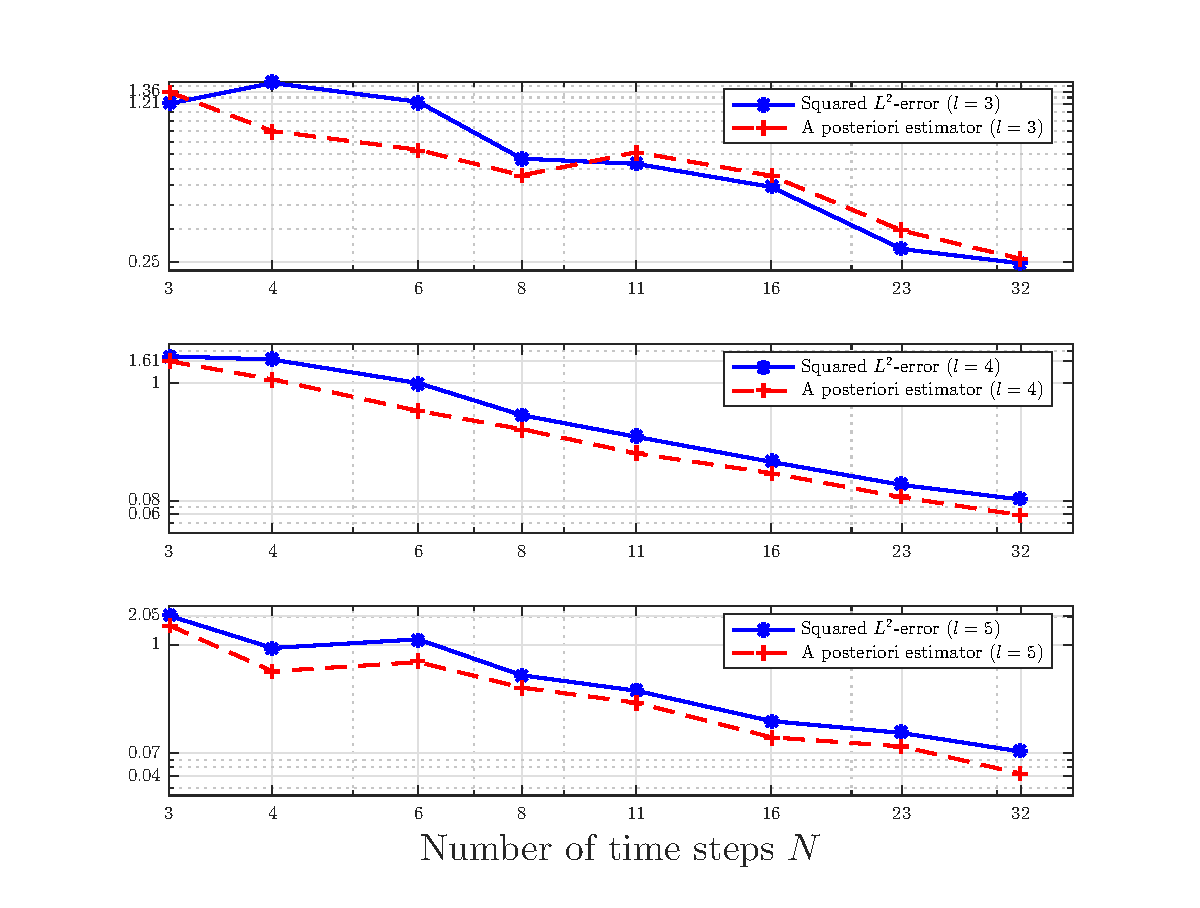
\includegraphics[height=8cm,keepaspectratio]{plot_diff_l_j_loglog}
\caption{
Comparison between the  squared $L^2$-error 
and  the \textit{a posteriori} error estimator with different 
time steps and sample sizes
(plotted in a log-log scale).}
\label{fig:TurePost}
\end{figure}

Figure \ref{fig:TurePost} compares  the  squared $L^2$-errors 
and  
the estimated squared errors (by using \eqref{eq:errorEstimate})
 for
numerical solutions obtained with 5 Picard iterations (i.e., $P=5$),
and
different  time steps $N$ and sample sizes $\Lambda$
as listed in \eqref{eq:NKLambda}.
We clearly observe that, for all choices of sample sizes,
the convergence behavior of  the estimated error 
and the true  error
are almost identical as  
the time stepsize tends to zero,
which confirms the theoretical results in Theorem \ref{thm:a_posterior_conts}.
Moreover, 
the ratio of the estimated error to the true error
suggests that,
for  this set of model parameters,
 the generic equivalence constant in Theorem \ref{thm:a_posterior_conts}
lies within the range of $0.7-1.2$,
which indicates that  the error estimator predicts  the  squared approximation error very accurately.
By performing linear regression of the estimated values (the dashed line) against the number of time steps,
we can infer 
without using the analytic solution of \eqref{eq:fbsde_lq}
that
 the approximation error 
 (in the $L^2$-norm)
 converges to zero at a rate of $N^{-0.7}$
 for the cases $l=4, 5$,
while for $l=3$, 
the approximation error also converges to zero but with a much slower rate.



Note that for general decoupled FBSDEs,
Corollary 1 in \cite{gobet2006} suggests  choosing the sample size $\Lambda$ corresponding to $l=5$  
in the least-squares Monte Carlo method
to achieve a half-order  $L^2$-convergence with respect to the number of time steps $N$.
Our numerical results indicate that,
%for the coupled MV-FBSDE \eqref{eq:fbsde_lq},
for the present example,
the convergence behaviour is  much better    than this theoretical error estimate,
possibly  due to a better time regularity of the process $Z$.
This suggests that one can design more efficient algorithms 
with tailored hyper-parameters
based on the error estimator \eqref{eq:errorEstimate}.
In particular, 
 \eqref{eq:errorEstimate}
 shows that 
 % for the current example,
%the choice
 $l=4$ leads to  the most efficient  algorithm  among the three choices of $l\in \{3,4,5\}$.
The cheaper algorithm with $l=3$ in general 
results in  significantly larger errors,
while
%compared with the choice $l=4$,
the choice $l=5$
not only requires a tremendously higher computational cost,
but also
achieves  almost the same  
accuracy as   the choice  $l=4$
 for  sufficiently fine grids;
for instance, with $N=32$ time steps, the error estimator predicts increasing $l$ from $4$ to $5$
will only reduce the squared error 
from 0.0586 to 0.0427,
% the accuracy by  0.016,
and in fact  the true squared error only reduces
from 0.0822 to 0.0734.
To illustrate the computational efforts  for the two choices $l=4,5$,
we present the 
corresponding
 sample size $\Lambda$
and  computational time
  with different numbers of time steps
in Table \ref{table:compare}.



\begin{table}[H]
 \renewcommand{\arraystretch}{1.05} 
\centering
\caption{ Sample size $\Lambda$ and computational time with different $N$ and $l$}
\label{table:compare}
\begin{tabular}[t]{@{}c c cc c cc@{}}
\toprule
 & \phantom{a}&  
 \multicolumn{2}{c}{$N=23$} &  \phantom{a}&  
 \multicolumn{2}{c}{$N=32$} \\
 \cmidrule{3-4} \cmidrule{6-7}
 $l$ & & Sample size  &   Run time & & Sample size &   Run time\\ \midrule
4 & & 32\,768  & 533s & & 	131\,072	& 3\,908s \\ 
5 & &  370\,728  & 5\,715s & & 	2\,097\,152	& 59\,338s \\ 
\bottomrule
\end{tabular}
\end{table}%
 

\begin{figure}[!ht]
\centering
\hspace{-12mm}
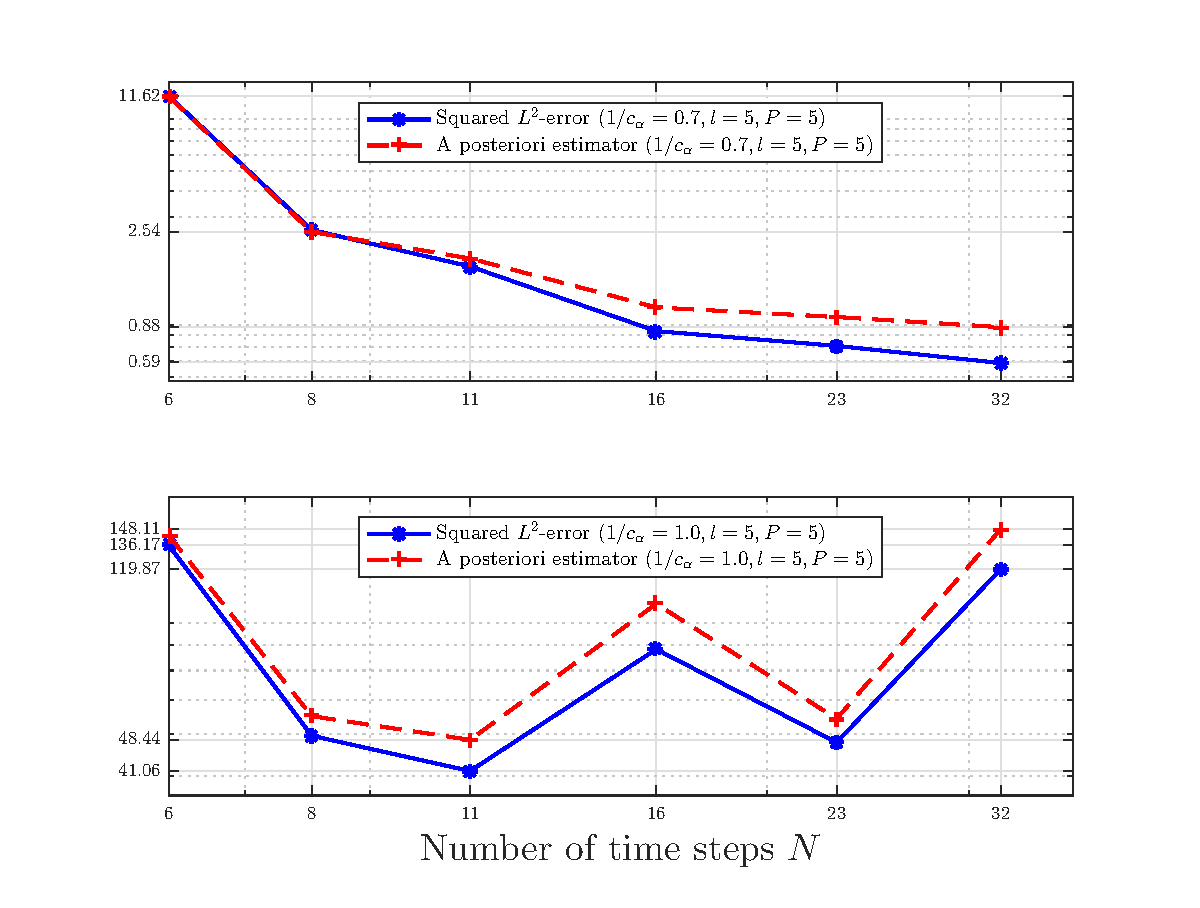
\includegraphics[trim=43 10 3 30, clip, width=0.54\columnwidth,keepaspectratio]{strong_coupling_c_alpha_2cases_P5}
\hspace{-7mm}
%height=9cm,
    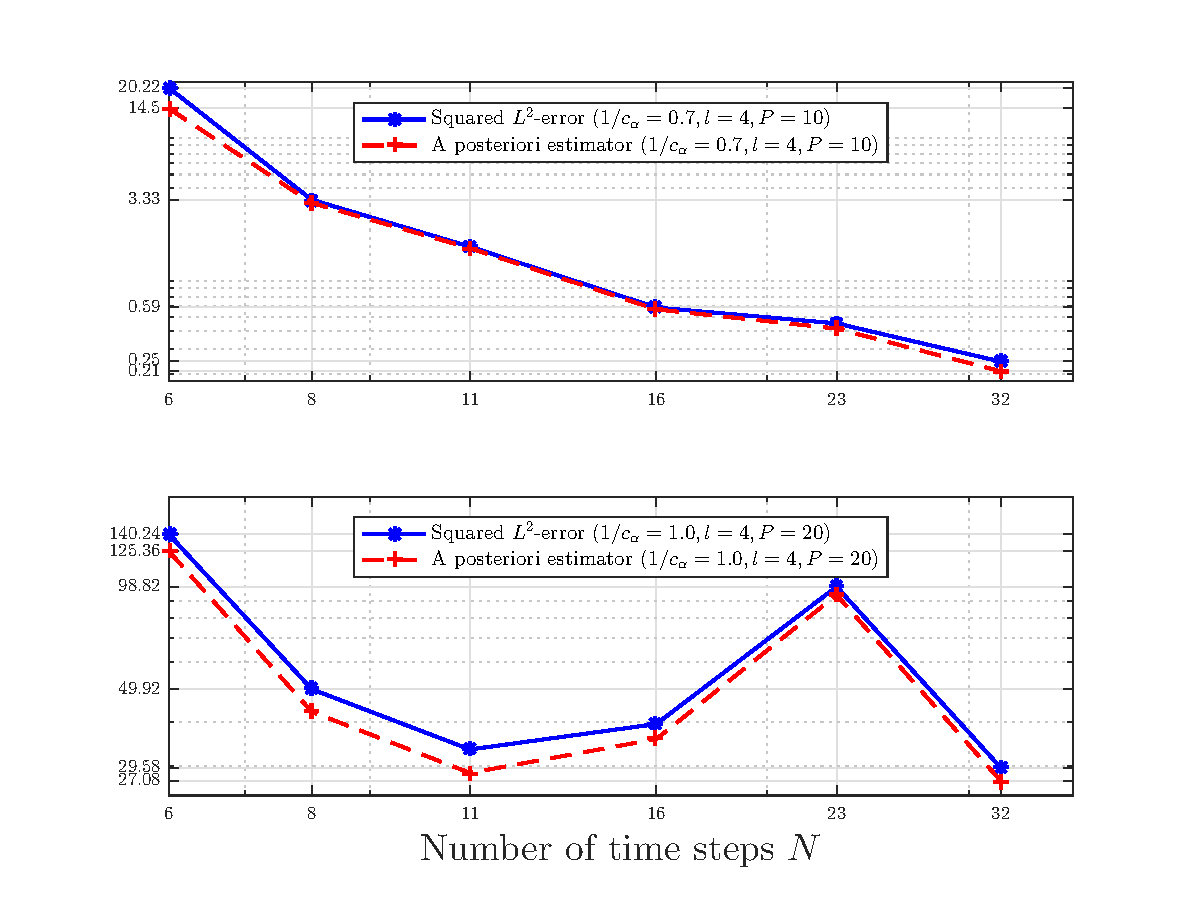
\includegraphics[trim=43 10 3 30, clip, width=0.54\columnwidth,keepaspectratio]{strong_coupling_c_alpha_2cases_Plarge}
\hspace{-20mm}    
%    keepaspectratio
\caption{
Robustness of  the \textit{a posteriori} error estimator for different
coupling parameters  $c_\alpha$
(plotted in a log-log scale);
from top to bottom: numerical results with $1/c_\a=0.7$ and  $1/c_\a=1.0$;
from left to right: numerical results with larger sample size ($l=5$) but fewer Picard iterations ($P=5$),
and numerical results with smaller sample size ($l=4$) but more Picard iterations.
}
\label{fig:coupling}
\end{figure}


 
We then proceed to examine the performance of the error estimator 
for MV-FBSDEs with  stronger coupling,
by varying the coefficient  $1/c_\alpha \in \{ 0.7, 1\}$
and keeping the other model parameters  as above.
Figure \ref{fig:coupling} (left) presents
the numerical results obtained by 
the hybrid algorithm  with
5 Picard iterations (i.e., $P=5$)
and
the discretization parameters $N, K,\Lambda$ as defined in \eqref{eq:NKLambda}
for $j=4,\ldots, 9$, $l=5$.
By comparison with 
the numerical results for $1/c_a=0.3$
(see Figure \ref{fig:TurePost}, bottom),
we can clearly observe  that
 as the coupling parameter $1/c_a$ increases,
 the  same choice of  discretization parameters
 leads to larger approximation errors.
%even though the true solution does not explode. 
The $L^2$-approximation error 
decays slowly for  the case with $1/c_{\alpha}=0.7$
as the number of time steps $N$ tends to infinity, 
while for  the case with $1/c_{\alpha}=1$,
the approximation errors  oscillate around
the value  $10^2$ 
and do not show   convergence 
for sufficiently large $N$.
Similar phenomena have been observed 
in \cite{andrea2019,chassagneux2019,germain2019},
where the authors found that  a stronger coupling between the forward and backward equations
can 
pose significant numerical challenges 
such as %bifurcations of numerical solutions or 
 slow convergence or even divergence of  Picard iterations.



More importantly, we see that the performance of the \textit{a posteriori} error estimator is very robust 
even for a large coupling parameter.
Regardless of the convergence of the hybrid algorithm,
the proposed error estimator captures the precise convergence behaviour of the true error
starting from a fairly small number of time steps,
and 
the ratio of the estimated error to the true error
generally stays in  the  range of $0.7-1$.
% as the previous test.
This enables us to judge the success of a given choice of discretization parameters 
without knowing the analytic solution to the problem.
In particular,  the error estimator suggests 
that for the case with $1/c_\alpha\in \{0.7,1\}$ and $P=5$,  the dominating error stems from other  sources 
(such as the Picard iteration)
instead of the time discretization or the  Monte Carlo regression.
Hence 
we cannot expect to significantly improve the approximation accuracy 
by keeping the number of Picard iterations fixed and  
only by
further refining the time grid or enlarging the sample size.


Motivated by the above observation,
we carry out the hybrid algorithm with 
 more Picard iterations 
($P=10$ for $1/c_\a=0.7$ and $P=20$ for $1/c_\a=1$)
but less simulation samples
($l=4$).
Figure \ref{fig:coupling} (right)
presents 
the numerical results for 
the discretization parameters $N, K,\Lambda$ as defined in \eqref{eq:NKLambda}
with $j=4,\ldots, 9$.
One can observe 
a significant improvement in the algorithm's efficiency
for the case with $1/c_\a=0.7$ (see Figure \ref{fig:coupling}, top-right),
where
the hybrid algorithm converges with a rate of $N^{-0.8}$
for the whole range of time steps,
and results in more accurate numerical solutions with less computational time
than the original choice of $P=5$, $l=5$ (see Figure \ref{fig:coupling}, top-left).
The situation is less clear for  the case with $1/c_\a=1$ (see Figure \ref{fig:coupling}, bottom-right).
Although the error is reduced by half
as compared to the choice of $P=5$ and $l=5$,
the error estimator does not decrease significantly starting from $N=11$,
which suggests that
more Picard iterations or a better scheme need to be employed for further improvements.















\section{Conclusions}

This paper proposes an \textit{a posteriori} error estimator to quantify the approximation accuracy 
of given discrete solutions to systems of
fully coupled MV-FBSDEs
arising from
optimization problems with a large population.
The error estimator applies to numerical solutions 
generated
from an arbitrary time-stepping scheme,
an arbitrary numerical procedure for approximating conditional expectations
and an arbitrary discrete
approximation of  Brownian increments.
We establish that 
the proposed error estimator is equivalent to 
the squared $L^2$-error between a given approximate solution 
and the true solution in a discrete-time setting,
and further demonstrate that
the  error estimator can effectively indicate 
the global approximation accuracy of  a given numerical solution 
 in a continuous-time setting.
 Numerical examples for an extended mean field game arising from optimal execution problems
  are presented to illustrate the theoretical findings
  and the practical applicability of the error estimator.

To the best of our knowledge, this is the first paper which carries out rigorous  
\textit{a posteriori} error estimates for 
systems of
fully coupled MV-FBSDEs with arbitrary terminal time.
The error estimates rely on a careful analysis of the corresponding discretized MV-FBSDE,
 which can be extended to derive 
  computable $L^p$-error bounds 
 for  fully coupled MV-FBSDEs driven by general martingales (see e.g.~\cite{el1997}).

A natural next step would be to design efficient numerical algorithms for solving fully-coupled MV-FBSDEs 
based on the \textit{a posteriori} error estimator. 
We have illustrated in the  numerical experiments 
that the proposed error estimator can enhance the efficiency of the algorithm by tailoring the hyper-parameters.
One can further develop adaptive strategies for using hierarchical basis functions in the approximation of  conditional expectations.

Another open question is a complete convergence analysis of 
the Deep BSDE Solver for solving fully-coupled MV-FBSDEs,
which has been recalled in Section \ref{sec:a_posteriori_conts}  (see also \cite{germain2019}).
In this paper we have made an initial step 
by showing that smaller terminal losses in the Deep BSDE Solver lead to more accurate solutions.
Further  research is needed to show an arbitrary small terminal loss can be attained in the computation,
which requires a careful analysis of the decoupling fields of the MV-FBSDEs.

























%\bibliography{bi}
%\bibliographystyle{plain}
\begin{thebibliography}{1}

\bibitem{andrea2019}
A. Andrea, C. Graves, H. Li, J.~F.~Chassagneux, F.~Delarue, and
R.~Carmona, \emph{Cemracs 2017: numerical probabilistic approach to MFG}, ESAIM:
Proceedings and Surveys, 65  (2019), pp. 84--113. 


\bibitem{bender2017}
C. Bender, N. Schweizer, and J. Zhuo, \emph{A primal-dual algorithm for BSDEs}, Math. Finance,
27 (2017), pp.~866--901.

\bibitem{bender2013}
C. Bender and J. Steiner, \emph{A posteriori estimates for backward SDEs}, SIAM/ASA J. Uncertain. Quantif.,
1 (2013), pp. 139--163.

\bibitem{bender2008}
C. Bender and J. Zhang, \emph{Time discretization and Markovian iteration for coupled FBSDEs},
Ann. Appl. Probab., 18 (2008), pp. 143--177.


\bibitem{bensoussan2015}
A. Bensoussan, S. Yam,  and Z. Zhang, \emph{Well-posedness of mean-field type forward-backward stochastic differential equations}, Stochastic Process. Appl., 125  (2015),
pp. 3327--3354.

\bibitem{bielecki2015}
T.~R.~Bielecki,  I.~Cialenco, and T.~Chen, \emph{Dynamic conic finance via backward stochastic difference equations},
SIAM J. Finan. Math., 6 (2015), pp. 1068--1122.

\bibitem{bouchard2004}
B. Bouchard and N. Touzi, 
\emph{Discrete time approximation and Monte Carlo simulation for backward
stochastic differential equations}, Stoch. Process. Appl., 111 (2004), pp. 175--206.


\bibitem{buckdahn2017}
R. Buckdahn, J. Li, S. Peng, and C. Rainer (2017), \emph{Mean-field stochastic differential equations
and associated PDEs}, Ann. Probab., 45, pp.~824--878.


\bibitem{carmona2013}
R. Carmona and F. Delarue, \emph{Mean field forward-backward stochastic differential equations},
Electron. Commun. Probab., 18 (2013), pp.~1--15.

\bibitem{carmona2013_siam}
R. Carmona and F. Delarue, \emph{Probabilistic analysis of mean-field games},
  SIAM J. Control Optim., 51 (2013), pp.~2705--2734. 


\bibitem{carmona2015}
R. Carmona and F. Delarue, \emph{Forward-backward stochastic differential equations and controlled McKean-Vlasov dynamics},
Ann. Probab., 43 (2015), pp.~2647--2700. 
  
\bibitem{carmona2018a} 
R.\ Carmona and F.\ Delarue, \emph{Probabilistic theory of mean field games with applications I: Mean-field FBSDEs, control, and games}, Springer International Publishing, Switzerland, 2018.
 



\bibitem{carmona2019}
R. Carmona and M.~Lauri\`{e}re, 
\emph{Convergence analysis of machine learning algorithms for the numerical solution of mean field control and games: II--The finite horizon case},  arXiv preprint, arXiv:1908.01613, 2019.

\bibitem{chassagneux2014}
J.~F.~Chassagneux, D.~Crisan, and F.~Delarue, 
\emph{A probabilistic approach to
classical solutions of the master equation for large population equilibria}, 
Mem. Amer. Math. Soc.,
(2020),
Available at
 arXiv:1411.3009.



\bibitem{chassagneux2019}
J.~F.~Chassagneux, D.~Crisan, and F.~Delarue, 
\emph{Numerical method for FBSDEs of McKean-Vlasov type}, 
Ann. Appl. Probab., 29 (2019), pp.~1640--1684.

\bibitem{chaudru2015}
P. E. Chaudru de Raynal and C. A. Garcia Trillos, 
\emph{A cubature based algorithm to solve decoupled McKean-Vlasov forward-backward stochastic differential equations}, Stochastic Process. Appl. 125 (2015), pp.~2206--2255.

\bibitem{delarue2006}
F. Delarue and S. Menozzi, \emph{A forward-backward stochastic algorithm for quasi-linear PDEs},
Ann. Appl. Probab., 16 (2006), pp.~140--184.

\bibitem{e2017}
W. E, J. Han, and A. Jentzen, \emph{Deep learning-based numerical methods for high-dimensional parabolic partial differential equations and backward stochastic differential equations}, Commun. Math. Stat., 5 (2017), pp. 349--380.


\bibitem{el1997}
N. El Karoui and S.-J. Huang, \emph{A general result of existence and uniqueness of backward
stochastic differential equations}, in Backward Stochastic Differential Equations, N. El
Karoui and L. Mazliak, eds., Longman, Harlow, 1997, pp. 27--36.



\bibitem{follmer2004}
H. F\"{o}llmer and A. Schied, \emph{Stochastic Finance. An Introduction in Discrete Time}, 2nd ed., de Gruyter,
Berlin, Germany, 2004.

\bibitem{fouque2019}
J.-P.~Fouque and Z.~Zhang, \emph{Deep learning methods for mean field control problems with delay},
  arXiv preprint, arXiv:1905.00358, 2019.


\bibitem{germain2019}
M. Germain, J. Mikael, and X.~Warin. \emph{Numerical resolution of McKean-Vlasov
FBSDEs using neural networks},
  arXiv preprint, arXiv:1908.00412, 2019.


\bibitem{gobet2006}
E.~Gobet, J.-P.~Lemor, and X.~Warin, \emph{Rate of convergence of an empirical regression method for
solving generalized backward stochastic differential equations}, Bernoulli, 12 (2006), pp. 889--916.



\bibitem{gnoatto2020}
A.~Gnoatto, C.~Reisinger, and  A.~Picarelli, \emph{Deep xVA Solver--A neural network based counterparty credit risk management framework},  Available at SSRN 3594076, 2020.



\bibitem{hajiali2018} 
A.-L.\ Haji-Ali and R.\ Tempone, 
\emph{Multilevel and Multi-index Monte Carlo methods for the McKean-Vlasov equation}, 
Stat. Comput, 28 (2018),  pp.~923--935.  

\bibitem{hamadene1999}
S. Hamad\`{e}ne, \emph{Nonzero sum linear-quadratic stochastic differential games and backward-forward
equations}, Stochastic Anal. Appl., 17 (1999), pp. 117--130.


\bibitem{han2018}
 J.~Han and J.~Long, \emph{Convergence of the deep BSDE method for coupled FBSDEs},
 arXiv preprint,  arXiv:1811.01165, 2018.




\bibitem{hure2020}
C.~Hur\'{e}, H.~Pham,  and X.~Warin, \emph{Some machine learning schemes for high-dimensional
nonlinear PDEs}, Math. Comp., 89 (2020), pp.~1547--1579.

%\bibitem{ji2019}
%S.~Ji,  and H.~Liu, H, \emph{Solvability of one kind of forward-backward stochastic difference equations}, arXiv preprint, arXiv:1901.02143, 2019.
%

\bibitem{ito2020}
K. Ito, C.~Reisinger, and Y. Zhang, \emph{A neural network based policy iteration algorithm with
global $H^2$-superlinear convergence for stochastic games on domains}, 
 Found. Comput. Math., (2020),
 Available at arXiv:1906.02304v3.


\bibitem{jacod1987}
J. Jacod and A.N. Shiryayev, \emph{Limit Theorems for Stochastic Processes}, Springer-Verlag, New
York, 1987.

\bibitem{ji2020}
S. Ji, S. Peng, Y. Peng and X. Zhang, \emph{Three algorithms for solving high-dimensional fully-coupled FBSDEs through deep learning}, IEEE Intelligent Systems, (2020).

\bibitem{lionnet2015}
A. Lionnet, G. dos Reis, and L. Szpruch, \emph{Time discretization of FBSDE with polynomial growth drivers and reaction-diffusion PDEs},  Ann. Appl. Probab.,  25  (2015), pp.~2563--2625.



\bibitem{peng1999}
S. Peng and Z. Wu, \emph{Fully coupled forward-backward stochastic differential equations and
applications to optimal control}, SIAM J. Control Optim., 37 (1999), pp. 825--843.

\bibitem{picarelli2020}
A. Picarelli and C. Reisinger,
\emph{Probabilistic error analysis for some approximation schemes to optimal control problems},
Systems Control Lett., 137 (2020) pp.~1--11.

%
%\bibitem{protter2004}
%P. Protter, \emph{Stochastic Integration and Differential Equations}, Springer-Verlag, New York, 2004.

\bibitem{robert2019}
C. Robert, P. Briand, A. Ghannoum, and C. Labart, 
\emph{Simulation of McKean-Vlasov BSDEs by Wiener chaos expansion}, 
Available at hal-01976770,
2019.

\bibitem{yong2010}
J. Yong, \emph{Forward-backward stochastic differential equations with mixed initial and terminal
conditions}, Trans. Amer. Math. Soc., 362 (2010), pp. 1047--1096.

\bibitem{zhang2004}
J. Zhang, \emph{A numerical scheme for BSDEs}, Ann. Appl. Probab. 14 (2004), pp.~459--488.



\end{thebibliography}

 
\end{document} 

The proof involves several technical calculations, and the detailed steps have been presented in Appendix 
for the sake of readability.


 A detailed
proof can be found in the appendix of the preprint version, which is available from
the authors upon request.

